%%===========================================================%%
%%                                                           %%
%%                   SYSTEMATIC ERRORS                       %%
%%                                                           %% 
%%===========================================================%%


\chapter{Systematic uncertainties}\label{chap:systematicErrors} 

\section{Luminosity}\label{sec:lumiSyst}
For determination of the systematic uncertainty of the integrated luminosity we use the results of dedicated study of data from vernier scans~\cite{lumiNote} performed during fill \#18915. These scans were targeted on providing a precise calculation of the luminosity and an estimate of its uncertainty for the elastic proton-proton scattering measurement~\cite{elasticNote}. From this study we learn that the effective cross-secton visible in the ZDC detectors is equal to 0.294~mb with 4\% systematic uncertainty. The number is different from the effective ZDC cross-section used in the initial calculation of the luminosity at STAR, equal to 0.264~mb. The ratio of these numbers is 1.114. One concludes that the initial calculations of the luminosity based on the comparison of the coincidence rate of the East and West ZDC detectors, were overestimated by factor 1.114. Therefore, for the cross-section calculation we use a corrected integrated luminosity - a nominal integrated luminosity divided by aforementioned factor.

Additional component of the systematic uncertainty on the integrated luminosity accounts for a consistency between integrated cross-section measured within reference fill \#18915, and measured with the entire dataset. The integrated cross-section measured using solely data from fill \#18915 is equal to
\begin{equation}
 \sigma_{\text{fid}}^{\text{CEP}} = 55.3\pm2.4~\text{mb},
\end{equation}
while using entire dataset we obtain
\begin{equation}
 \sigma_{\text{fid}}^{\text{CEP}} = 51.3\pm0.4~\text{mb}.
\end{equation}
The absolute and relative difference between the two is, respectively,
\begin{equation}
 \Delta\sigma_{\text{fid}}^{\text{CEP}} = 4.0\pm2.4~\text{mb},~~~~~~~~~\Delta\sigma_{\text{fid}}^{\text{CEP}}/\sigma_{\text{fid}}^{\text{CEP}} = \left(7.8\pm4.7\right)~\%.
\end{equation}

Finally, the total systematic uncertainty of the integrated luminosity is a quadratic sum of generic uncertainty equal to 4\%, and uncertainty arising from the consistentsy between cross-section measured using data from fill \#18915 and entire dataset, equal to 7.8\%:

\begin{equation}
\Delta\mathcal{L}/\mathcal{L} = 4.0\%\oplus7.8\% = 8.8\%. 
\end{equation}


\begin{figure}[h]
\centering
\includegraphics[width=.48\textwidth,page=2]{graphics/systematics/sigmaVsRunNumber.pdf}~~~~%
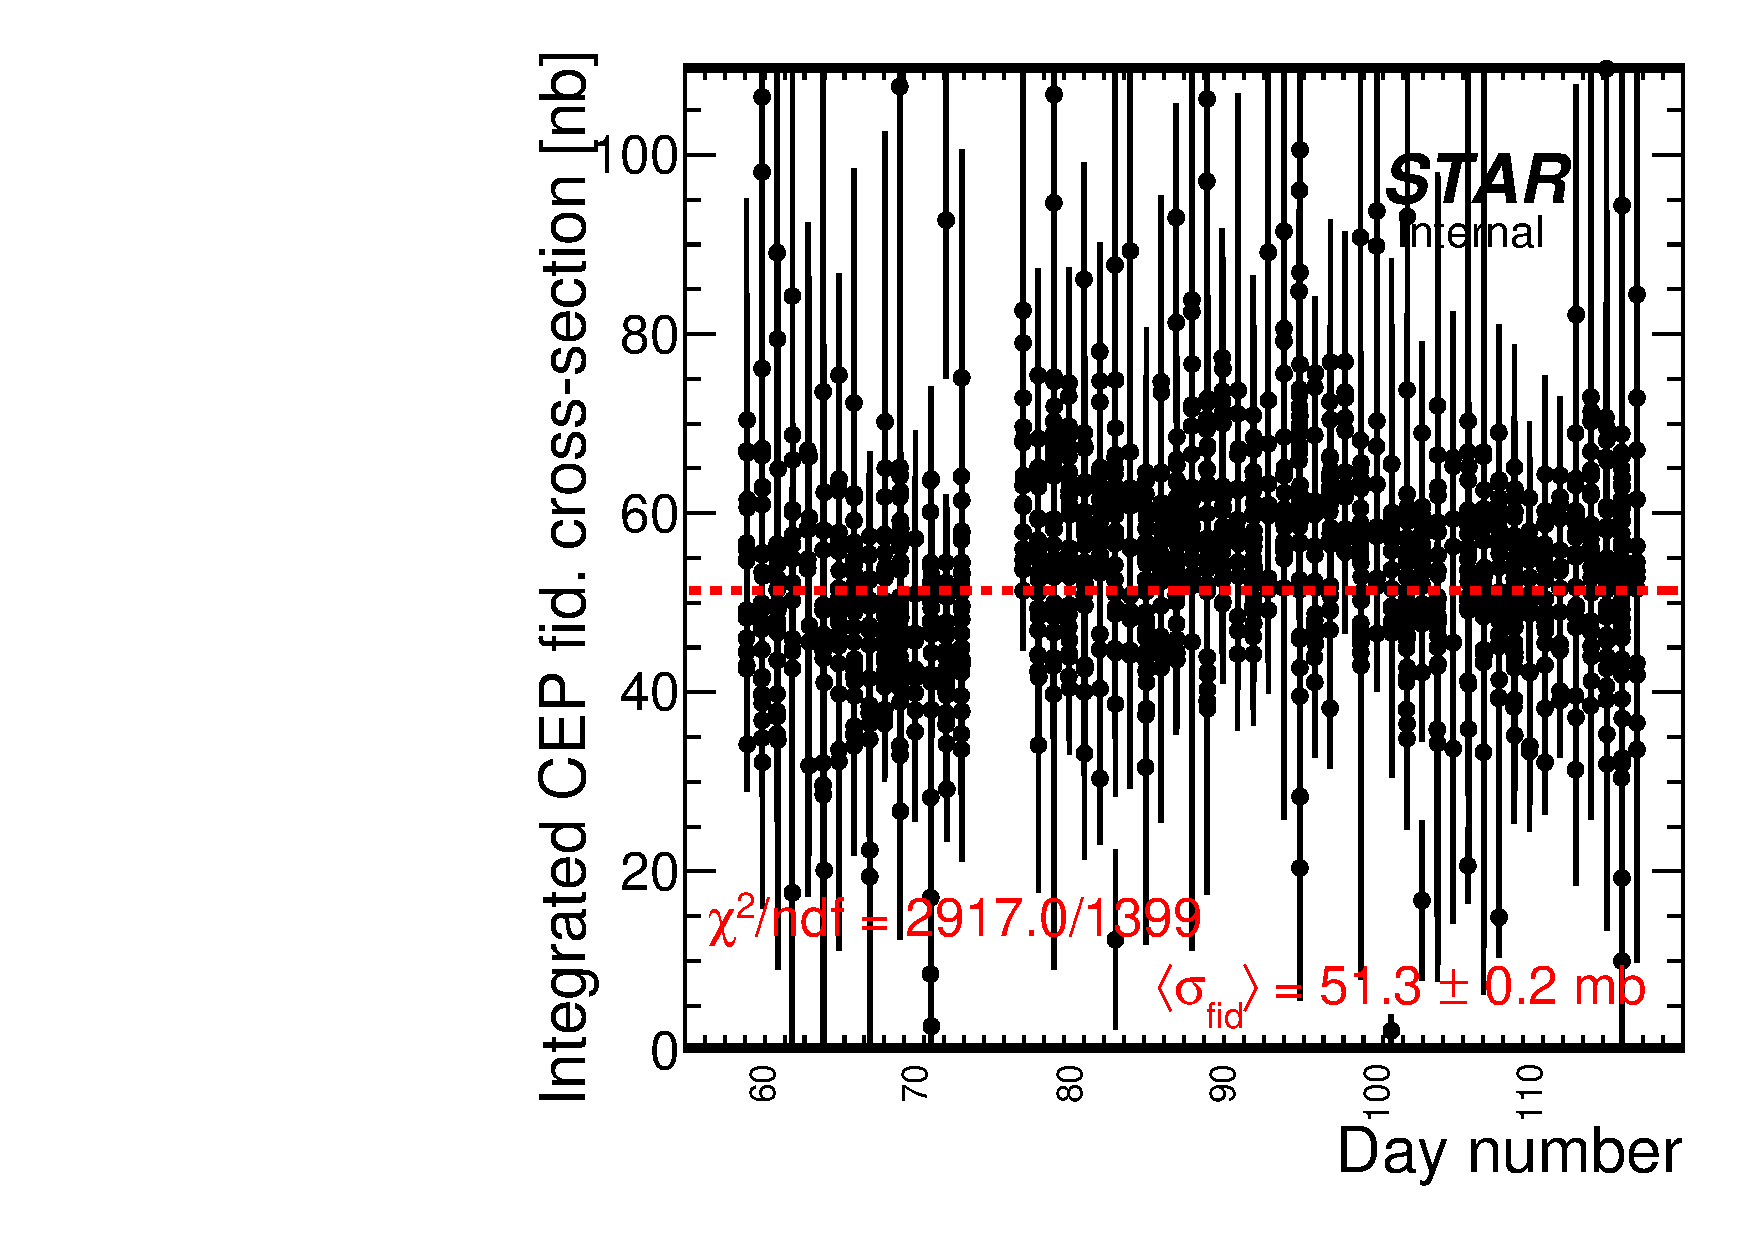
\includegraphics[width=.48\textwidth,page=1]{graphics/systematics/sigmaVsRunNumber.pdf}% 
\caption[Luminosity uncertainty systematics.]{Integrated fiducial CEP cross-section for runs from fill \#18915~(left) and for all runs~(right).}
\label{fig:lumiSyst}
\end{figure}


\section{Trigger veto effect (due to dead material)}\label{sec:systTrigVeto}

Systematic uncertainty related to the trigger veto correction (Sec.~\ref{sec:rpDeadMat}) has been studied with elastic scattering events, in a way similar to analyses presented in Sec.~10.3 (and following) of Ref.~\cite{supplementaryNote}. 

Triggers dedicated for elastic scattering process (RP\_ET triggers) have been studied. The trigger required signal in at least one PMT (out of four) in two RP branches opposite to each other with respect to interaction region. In addition to trigger selection, vetoes were imposed offline on any activity in other STAR detectors, such as BBC (small and large), ZDC, TOF and VPD - it reduced probability of a non-elastic pile-up interaction. It has been demonstrated in Sec.~10.3.1 of Ref.~\cite{supplementaryNote} that once the single good quality RP track is required on one side, such sample consists only of elastic proton-proton scattering events.

Each side (branch) was analyzed independently; when single good quality RP track, in addition of $|\xi|<0.01$, was found on the east side, the systematics for west side was investigated (and vice versa). Two histograms were filled per event. The first histogram was filled with all selected events. The second histogram was filled only if there was no simultaneous signal in upper and lower RP on studied side (no ET and IT trigger bits fired at the same time) - just the same, as it was implemented in RP\_CPT2 trigger. However, the second histogram was filled with weight equal to inverse efficiency of the veto, $1/\mbox{\LARGE$\epsilon$}_{\text{DM~veto}}^{\text{side}}$. The ratio of the second to first histogram,
\begin{equation}
 R_{\text{DM~veto}} = \frac{\text{histogram of events with satisfied veto, filled with weight } 1/\mbox{\LARGE$\epsilon$}_{\text{DM~veto}}^{\text{side}}}{\text{histogram of all events, filled with unit weight}},
\end{equation}
has been presented in Fig.~\ref{fig:systDMveto} as a function of $p_{x}$ and $p_{y}$ of elastically scattered proton on studied side. If single good quality proton track was reconstructed in studied branch, parameters of that track were histogrammed. Otherwise, transverse components of momentum of unreconsructed elastic proton (e.g. due to induced shower) were estimated as $-p_{x}$ and $-p_{y}$ of elastic proton track on the opposite side.

\begin{figure}[h]
\centering
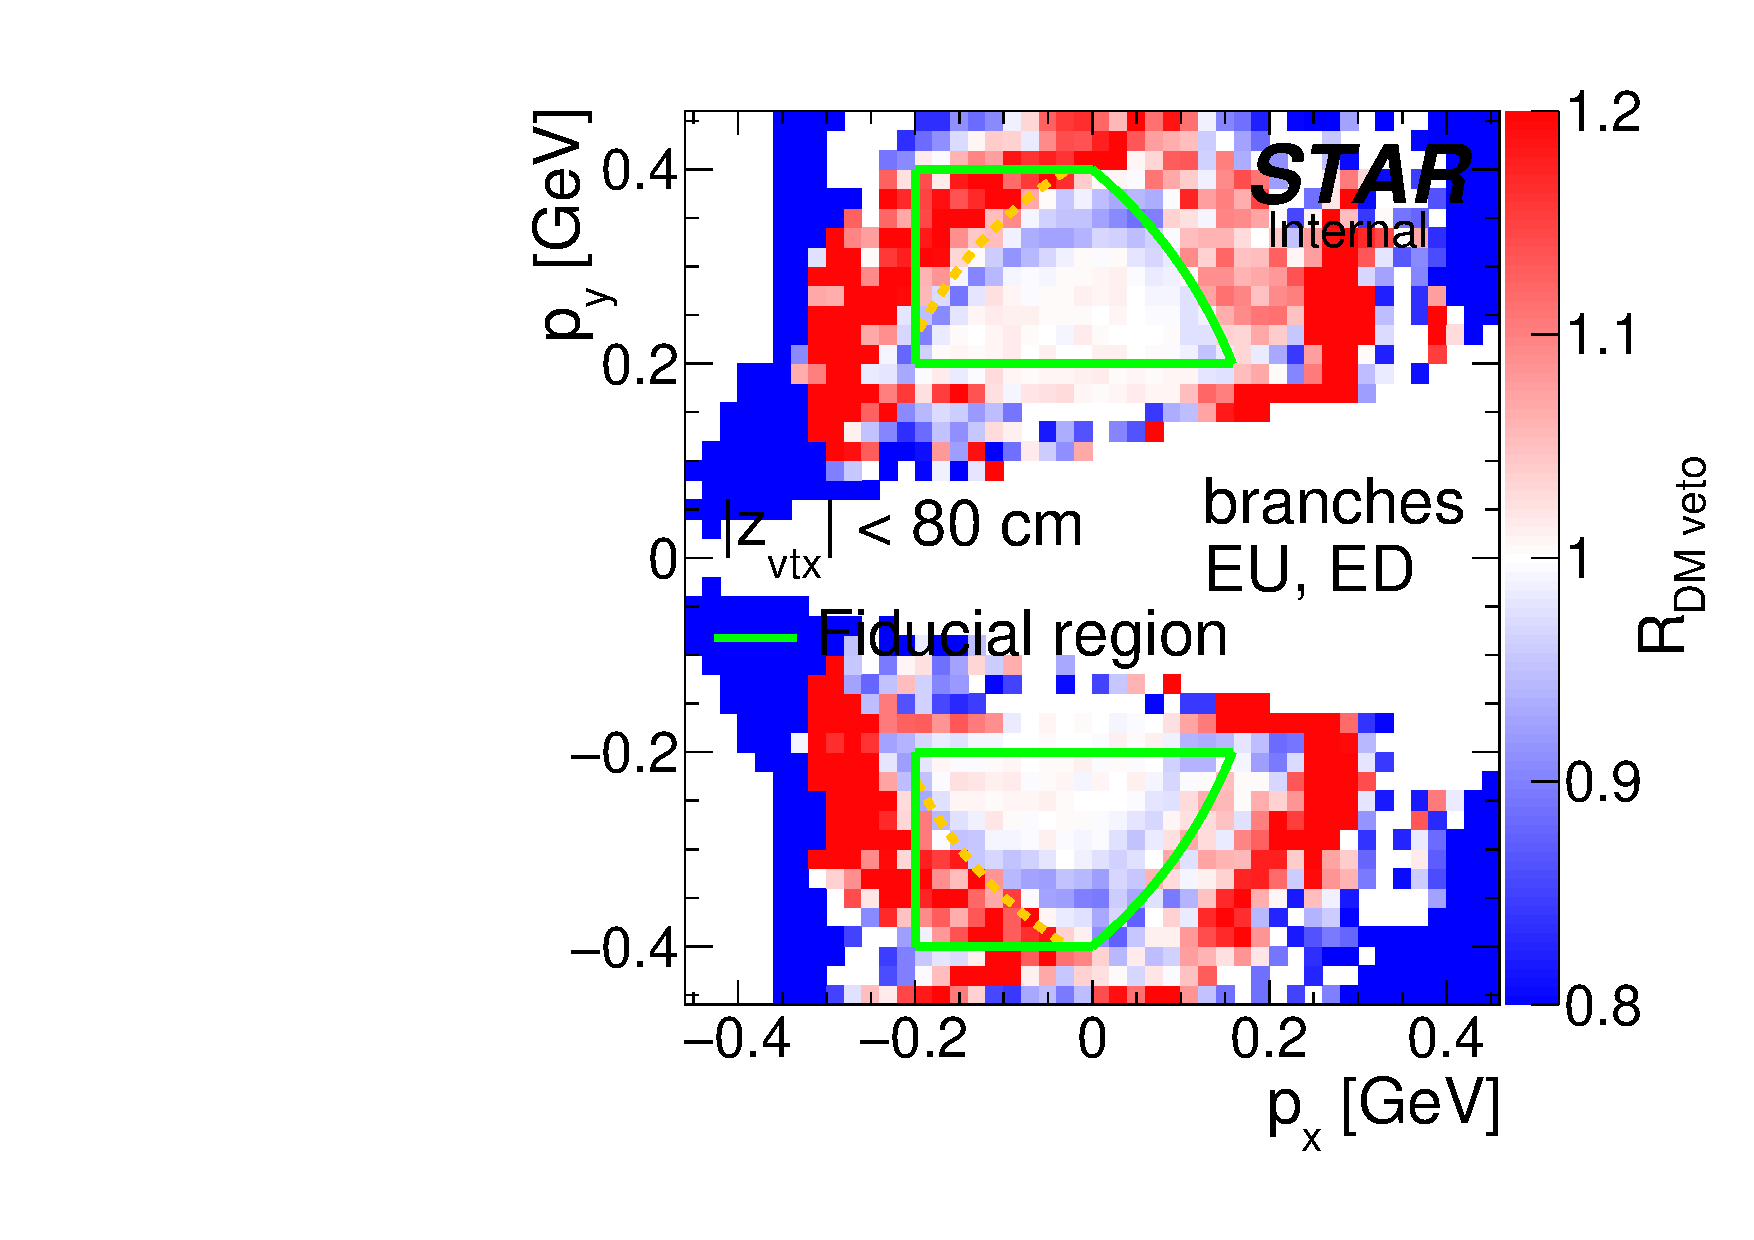
\includegraphics[width=.48\textwidth,page=1]{graphics/systematics/deadMatSyst.pdf}~~~~%
\includegraphics[width=.48\textwidth,page=2]{graphics/systematics/deadMatSyst.pdf}%
\caption[Estimated systematic uncertainty related to trigger veto induced by interaction with dead material.]{Ratio $R_{\text{DM~veto}}$ illustrating systematic uncertainty of the dead material trigger veto correction in east (left) and west (right) Roman Pots.}
\label{fig:systDMveto}
\end{figure}

Results presented in Fig.~\ref{fig:systDMveto} indicate imperfect description of the dead material of the elements surrounding RPs (DX-D0 chamber, RF shield), which has been also overved in studies of systematic uncertainties related to RP track reconstruction efficiency, presented in Ref.~\cite{supplementaryNote}. Based on current study, the correction and systematic uncertainty of the dead material veto efficiency $\mbox{\LARGE$\epsilon$}_{\text{DM~veto}}^{\text{side}}$ are assumed to have the following form: 
\begin{itemize}
\item multiplicative correction is applied to $\mbox{\LARGE$\epsilon$}_{\text{DM~veto}}^{\text{side}}$, equal to $1+\frac{1}{2}(R_{\text{DM~veto}}-1)$,
 \item systematic uncertainty is assumed to be equal to $1+\frac{1}{2}|R_{\text{DM~veto}}-1|$, therefore propagation of this systematic effect is done by variating the efficiency $\mbox{\LARGE$\epsilon$}_{\text{DM~veto}}^{\text{side}}$ by the multiplicative factor equal to $\pm\left[1+\frac{1}{2}|R_{\text{DM~veto}}-1|\right]$. 
\end{itemize} 


\section{TPC track quality cuts variation}\label{sec:systTpcQuaCuts}

We have tested senstivity of the fiducial cross-sections on the variation of the quality cuts used in TPC track selection. Any change of these cuts requires re-calculation of the TPC track reconstruction and TOF matching efficiencies (the latter is conditional w.r.t. the former). We have checked two working points, 'loose' and 'tight, with different set of cuts on $d_{0}$, $N_{\text{fit}}^{\text{hits}}$ and $N^{\text{hits}}_{\text{dE/dx}}$ compared to nominal working point. Definition of 'loose' and 'tight' cuts is provided in Sec.~3.2.4 of Ref.~\cite{supplementaryNote}, together with depiction of resulted changes of the efficiencies.

Observed ratios of the cross-sections obtained with modified cuts and accordingly redefined TPC and TOF efficiencies, to the nominal cross-section, are shown in Fig.~\ref{fig:tpcQuaVariation}. The upward and downward relative changes of the cross-sections were added in quadrature. The resulting systematic uncertainty of the cross-section related to TPC track quality cuts is estimated to be $^{+2.0}_{-1.5}\%$.
 
\begin{figure}[h]
\centering
\includegraphics[width=.8\textwidth,page=2]{graphics/systematics/TrackQualityCutVariation_InvMass.pdf}
%
\caption[Result of variation of the TPC track quality cuts on $d\sigma/dm(\pi^{+}\pi^{-})$.]{Result of variation of the TPC track quality cuts on the fiducial differential exclusive $\pi^{+}\pi^{-}$ production cross-section as a function of the invariant mass of $\pi^{+}\pi^{-}$. Dashed horizontal lines respresent an average ratio for a modified cut marked with the same color.}
\label{fig:tpcQuaVariation}
\end{figure}


%%%%%%%%%%%%%%%%%%%%%%%%%%%%%%%%%%%%%%%%%% 

\section{Discussion of systematic effects}\label{sec:systEffectsList}
The following contributions to the overall systematic uncertainty have been studied. Influence of each systematic effect on measured cross sections has been tested by changing amount of the quantity that the systematic effect refers to and comparing the result with that obtained using nominal values.

\begin{enumerate}
 \item \textbf{Representativeness of the embedding sample ($\bm{\Delta\varepsilon_{\text{TPC}}}$ (embed. stat.)).}\\
 Zero-bias data available for the MC embedding is only a fraction of all zero-bias triggers, therefore physics data may be not fully represented in MC events used for determination of the TPC track reconstruction efficiency. This effect was studied by comparing estimated average levels of pile-up in the data and embedded MC. The difference was found to be of the order of 1\%, which we establish as a symmetric systematic uncertainty on the TPC track reconstruction efficiency (per track). See the last paragraph of Sec.~10.1.1 of Ref.~\cite{supplementaryNote} for more details.
 %
 \item \textbf{Embedding procedure/off-time pile-up effect ($\bm{\Delta\varepsilon_{\text{TPC}}}$ (pile-up)).}\\
 Reliability and precision of the embedding technique was verified and quantitatively estimated in the procedure described in Sec.~10.1.1 of Ref.~\cite{supplementaryNote}. Embedded MC samples were divided into sub-samples representing different levels of off-time pile-up/densitity of hit points in TPC. With dedicated analysis it was possible to verify if the TPC track reconstruction efficiency is compatible between all sub-samples when the effect of pile-up (changing number of hits forming a track) is reduced. The average systematic uncertainty related to the embedding procedure is $<1\%$ (per track, Fig.~10.5 of Ref.~\cite{supplementaryNote}).
 %
 \item \textbf{Modelling of the dead material in front of the TPC ($\bm{\Delta\varepsilon_{\text{TPC}}}$ (dead mat.)).}\\
 Not all detector elements are fully modeled in the MC simulation, quite often some simplifications are used. This leads to inaccuracies in efiiciencies derived from the simulation. We estimated systematic uncertainty related to amount of simulated material between the primary vertex and STAR TPC to be 25\% which translates to $\approx 0.5\%$ of uncertainty of the TPC track reconstruction efficiency. See Chap.~9 of Ref.~\cite{supplementaryNote} for details.
 %
 \item \textbf{Modelling of TPC track quality parameters in embedded MC ($\bm{N^{\text{hits}}}$ and $\bm{d_{0}/\text{DCA}(R)}$).}\\
 We have checked the impact of variation of the track quality cuts on the obtained cross-sections. It reflects systematic uncertainty related to the quality of modeeling of the quantities used to select the primary TPC tracks. The estimated uncertainty on the fiducial cross-section amounts $^{+2.0}_{-1.5}\%$. See Sec.~\ref{sec:systTpcQuaCuts}.
  %
 \item \textbf{Vertexing ($\bm{\Delta\epsilon_{\text{vtx}}}$).}\\
 Vertexing efficiency has been obtained using data-driven method presented in Sec.~\ref{sec:tpcVxRecoEff}, thus systematic uncertainty related to this efficiency has been significantly reduced. Systematic uncertainty has been estimated as a difference between efficiency with and without subtracted background.
 %
 \item \textbf{Modelling of the TOF system and validity of derived efficiency corrections ($\bm{\Delta\varepsilon_{\text{TOF}}}$).}\\
 The efficiency of matching TOF hits with the TPC tracks has been extracted from embedded MC sample. It has been confronted with TOF efficiency extracted from the data using two independent techniques: tag\&probe (Sec.~4.1 of Ref.~\cite{supplementaryNote}) and HFT-tagging (Sec.~10.2.2 of Ref.~\cite{supplementaryNote}). Average difference between the data and MC efficiency has been used as a correction to MC efficiency, while half of the difference between data-extracted efficiencies has been treated as a systematic uncertainty (Fig.~10.16, Ref.~\cite{supplementaryNote}). This amounts 1\%-3\% (per track), depending on particle species.
%
 \item \textbf{Modelling of the RP system and validity of derived efficiency corrections ($\bm{\Delta\varepsilon_{\text{RP}}}$, $\bm{\Delta\varepsilon_{\text{RP}}^{\text{trig.}}}$ and $\bm{\Delta\varepsilon_{\text{RP}}^{\text{DM veto}}}$).}\\
 Reliability of RP simulation which was used to extract efficiency corrections with MC embedded into zero-bias data, has been verified and quantitatively estimated in the procedure described in Sec.~10.3 of Ref.~\cite{supplementaryNote}. For this purpose elastic proton-proton scattering events have been used. The same analysis has been performed on embedded elastic scattering MC and the data, leading to estimates of the RP acceptance and track reconstruction efficiency. The differences between two results has been considered as a measure of the systematic uncertainty that covers RP track reconstruction efficiency itself, detectors alignment, embedding technique. Similar studies have been performed to determine systematic uncertainty related to the trigger veto efficiency correction, as presented in Sec.~\ref{sec:systTrigVeto}.
 %
 \item \textbf{Pile-up veto correction ($\bm{\Delta\epsilon_{\text{veto}}}$).}\\
 Luminosity-dependent correction related to veto of pile-up interactions is derived from the zero-bias data on run by run basis. Residual systematic uncertainty has been estimated as a difference between the correction factor calculated for particular run, and correction factor obtained from the exponential fit to all points representing correction factors as a function of instantaneous luminosity.
 %
 \item \textbf{Longitudinal shape and position of the primary vertex distribution ($\bm{\Delta\langle z_{\text{vtx}}\rangle}$ and $\bm{\Delta\sigma( z_{\text{vtx}})}$).}\\
 Comparison of the $z_{\text{vtx}}$ distribution as seen in the TPC and in RPs leads to conservative estimate of the uncertainty of central position of the vertex equal 2~cm, and the spread (standard deviation) of vertex equal 3~cm.
 %
 \item \textbf{Non-exclusive background estimate ($\bm{\Delta N_{\text{bkgd}}^{\text{non-excl}}}$).}\\
 As explained in Sec.~\ref{sec:nonExclBkgdDetermination}, estimated systematic difference between real level of non-exclusive background, and level determined with a data-driven method, may be as high as 10\%. We apply such variation of the non-exclusive background and assign resulting differences of cross sections as their systematic uncertainty related to non-exclusive background determination method.
 %
 \item \textbf{Luminosity determination ($\bm{\Delta\mathcal{L}}$).}\\
 Uncertainty of the integrated luminosity has been estimated to 7\%, which is still subject to change.
\end{enumerate}

\section{Graphical representation of systematic uncertainties}
In this section we present relative contributions of effects listed in Sec.~\ref{sec:systEffectsList} to the total systematic uncertainties on differential fiducial cross sections presented in Chap.~\ref{chap:physicsResults}. Numbering of figures is preserved with respect to corresponding cross section results in the next chapter. The color code is the same in all figures, with the legend explaining the meaning of each color attached at the bottom of Fig.~\ref{systematics_01}.


\begin{figure}[h]
\centering
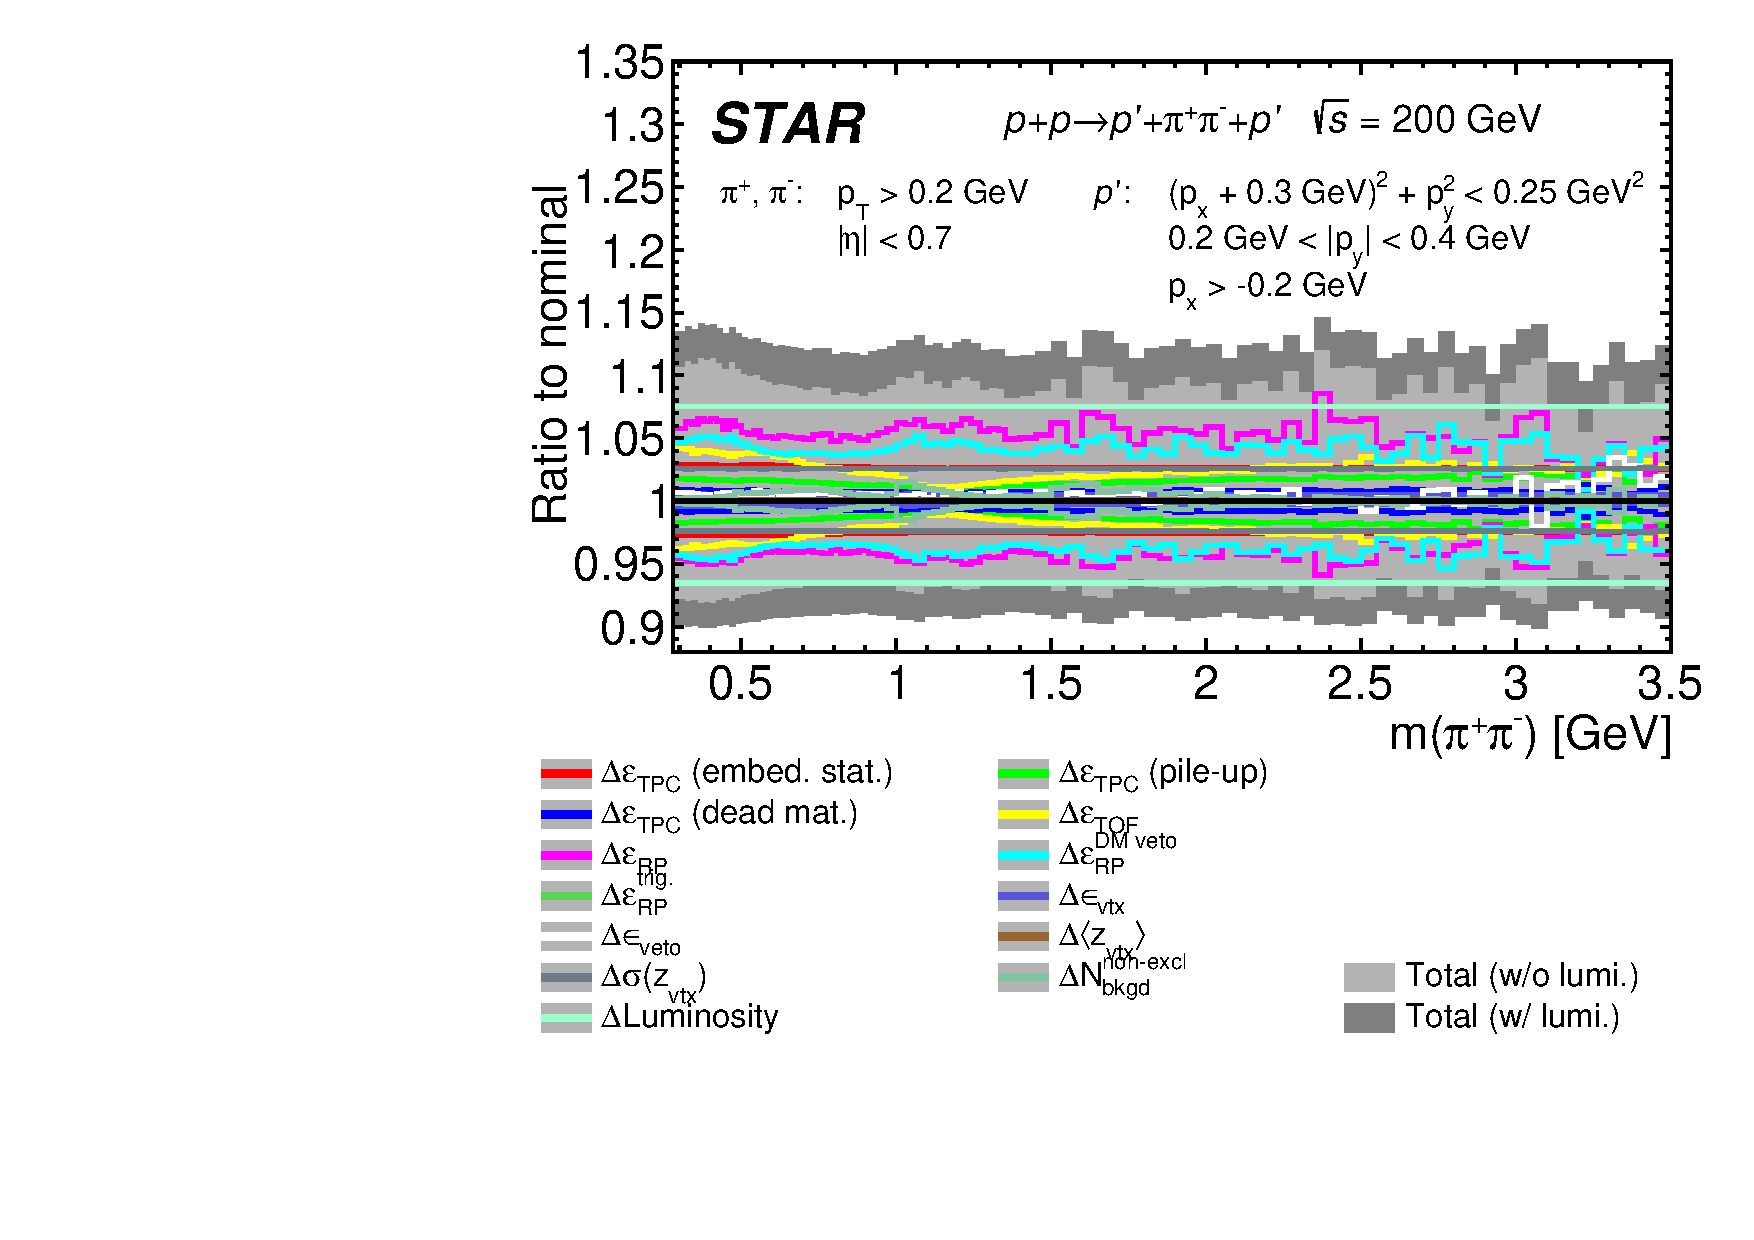
\includegraphics[width=.9\textwidth,page=1]{graphics/systematics/FinalResult_InvMass_pion_Systematics.pdf}
%
\caption{Systematic uncertainties of the differential cross sections for CEP of charged particle pairs $\pi^+\pi^-$ as a function of the invariant mass of the pair in the fiducial region explained on the plots.}
\label{systematics_01}
\end{figure}

% {
% \renewcommand{\arraystretch}{1.5}
% \begin{table}[]\centering
% \begin{tabular}{cc T{1.4cm}T{1.4cm}T{1.4cm} T{1.4cm}T{1.4cm}T{1.4cm}}
% \multicolumn{2}{c}{~}   & \multicolumn{3}{c}{$\bm{\Delta\varphi<90^{\circ}}$} &  \multicolumn{3}{c}{$\bm{\Delta\varphi>90^{\circ}}$}  \\
%     \multicolumn{2}{c}{~}  & \multicolumn{1}{c}{$\bm{\pi^{+}\pi^{-}}$} & \multicolumn{1}{c}{$\bm{K^{+}K^{-}}$} & \multicolumn{1}{c}{$\bm{p\bar{p}}$} & \multicolumn{1}{c}{$\bm{\pi^{+}\pi^{-}}$} & \multicolumn{1}{c}{$\bm{K^{+}K^{-}}$} & \multicolumn{1}{c}{$\bm{p\bar{p}}$} \\ \hline\hline
% \multirow{6}{*}{  \specialcell{ $\bm{ \frac{\delta_{\text{\bf{syst}}}}{\sigma_{\text{\bf{fid}}}} }$ \\ $\bm{[\text{\bf{\%}}]}$ }   } &  TOF & $\prescript{3.1}{-2.9}{~~~}$ & $\prescript{10.0}{-8.6}{~~~}$ & $\prescript{5.4}{-4.9}{~~~}$ & $\prescript{2.7}{-2.5}{~~~}$ & $\prescript{10.3}{-8.9}{~~~}$ & $\prescript{5.7}{-5.2}{~~~}$  \\
% &  TPC  & $\prescript{3.3}{-3.1}{~~~}$ & $\prescript{6.6}{-6.1}{~~~}$ & $\prescript{3.6}{-3.4}{~~~}$ & $\prescript{3.2}{-3.1}{~~~}$ & $\prescript{6.3}{-5.8}{~~~}$ & $\prescript{3.6}{-3.5}{~~~}$ \\
% &  RP  &  $\prescript{7.3}{-6.1}{~~~}$ & $\prescript{7.4}{-6.2}{~~~}$ & $\prescript{8.4}{-6.9}{~~~}$ & $\prescript{6.3}{-5.4}{~~~}$ & $\prescript{6.9}{-5.8}{~~~}$ & $\prescript{7.0}{-5.2}{~~~}$ \\
% &  Other  & $\prescript{2.6}{-2.4}{~~~}$ & $\prescript{2.7}{-2.4}{~~~}$ & $\prescript{2.9}{-2.4}{~~~}$ & $\prescript{2.6}{-2.4}{~~~}$ & $\prescript{2.6}{-2.4}{~~~}$ & $\prescript{3.2}{-2.4}{~~~}$ \\
% & Lumi. & \multicolumn{6}{c}{$7.0$} \\ \cline{2-8}
% &  Total & $\prescript{11.4}{-10.5}{~~~}$ & $\prescript{16.0}{-14.3}{~~~}$ & $\prescript{13.0}{-11.8}{~~~}$ & $\prescript{10.7}{-10.0}{~~~}$ & $\prescript{15.8}{-14.2}{~~~}$ & $\prescript{12.4}{-11.6}{~~~}$  \\ 
% \end{tabular}
% \caption{Systematic uncertainties of integrated fiducial cross sections for CEP of $\pi^{+}\pi^{-}$, $K^{+}K^{-}$ and $p\bar{p}$ pairs in two ranges of azimuthal angle difference $\Delta\varphi$ between forward scattered protons. Provided numbers are decomposed into major components. Single number in a cell indicates symmetric uncertainty, while positive and negative number denotes asymmetric uncertainty.}\label{tab:xSecSyst}
% \end{table}
% } 



{
\renewcommand{\arraystretch}{1.5}
\begin{table}[]\centering
\begin{tabular}{c ccccc|c}
 ~ & \multicolumn{6}{c}{  $\bm{ \delta_{\text{\bf{syst}}}/\sigma_{\text{\bf{fid}}}~[\text{\bf{\%}}]}$   } \\
 ~ & \bf{TOF} & \bf{TPC} & \bf{RP} & \bf{Other} & \bf{Lumi.} & \bf{Total} \\ \hline\hline
$\bm{\pi^{+}\pi^{-}}$ & $\prescript{3.1}{-2.9}{~~~}$ & $\prescript{3.3}{-3.1}{~~~}$ & $\prescript{7.3}{-6.1}{~~~}$ & $\prescript{2.6}{-2.4}{~~~}$ & \multirow{3}{*}{$\prescript{7.5}{-6.5}{~}$} & $\prescript{11.4}{-10.5}{~~~}$  \\
$\bm{K^{+}K^{-}}$  & $\prescript{10.0}{-8.6}{~~~}$ & $\prescript{6.6}{-6.1}{~~~}$ & $\prescript{7.4}{-6.2}{~~~}$ & $\prescript{2.7}{-2.4}{~~~}$ &  & $\prescript{16.0}{-14.3}{~~~}$ \\
$\bm{p\bar{p}}$  &  $\prescript{5.4}{-4.9}{~~~}$ & $\prescript{3.6}{-3.4}{~~~}$ & $\prescript{8.4}{-6.9}{~~~}$ & $\prescript{2.9}{-2.4}{~~~}$ &  & $\prescript{13.0}{-11.8}{~~~}$ \\
\end{tabular}
\caption{Typical systematic uncertainties of integrated fiducial cross sections for CEP of $\pi^{+}\pi^{-}$, $K^{+}K^{-}$ and $p\bar{p}$. Provided numbers are decomposed into major components. Single number in a cell indicates symmetric uncertainty, while positive and negative number denotes asymmetric uncertainty.}\label{tab:xSecSyst}
\end{table}
}


%
\begin{figure}[h]
\centering
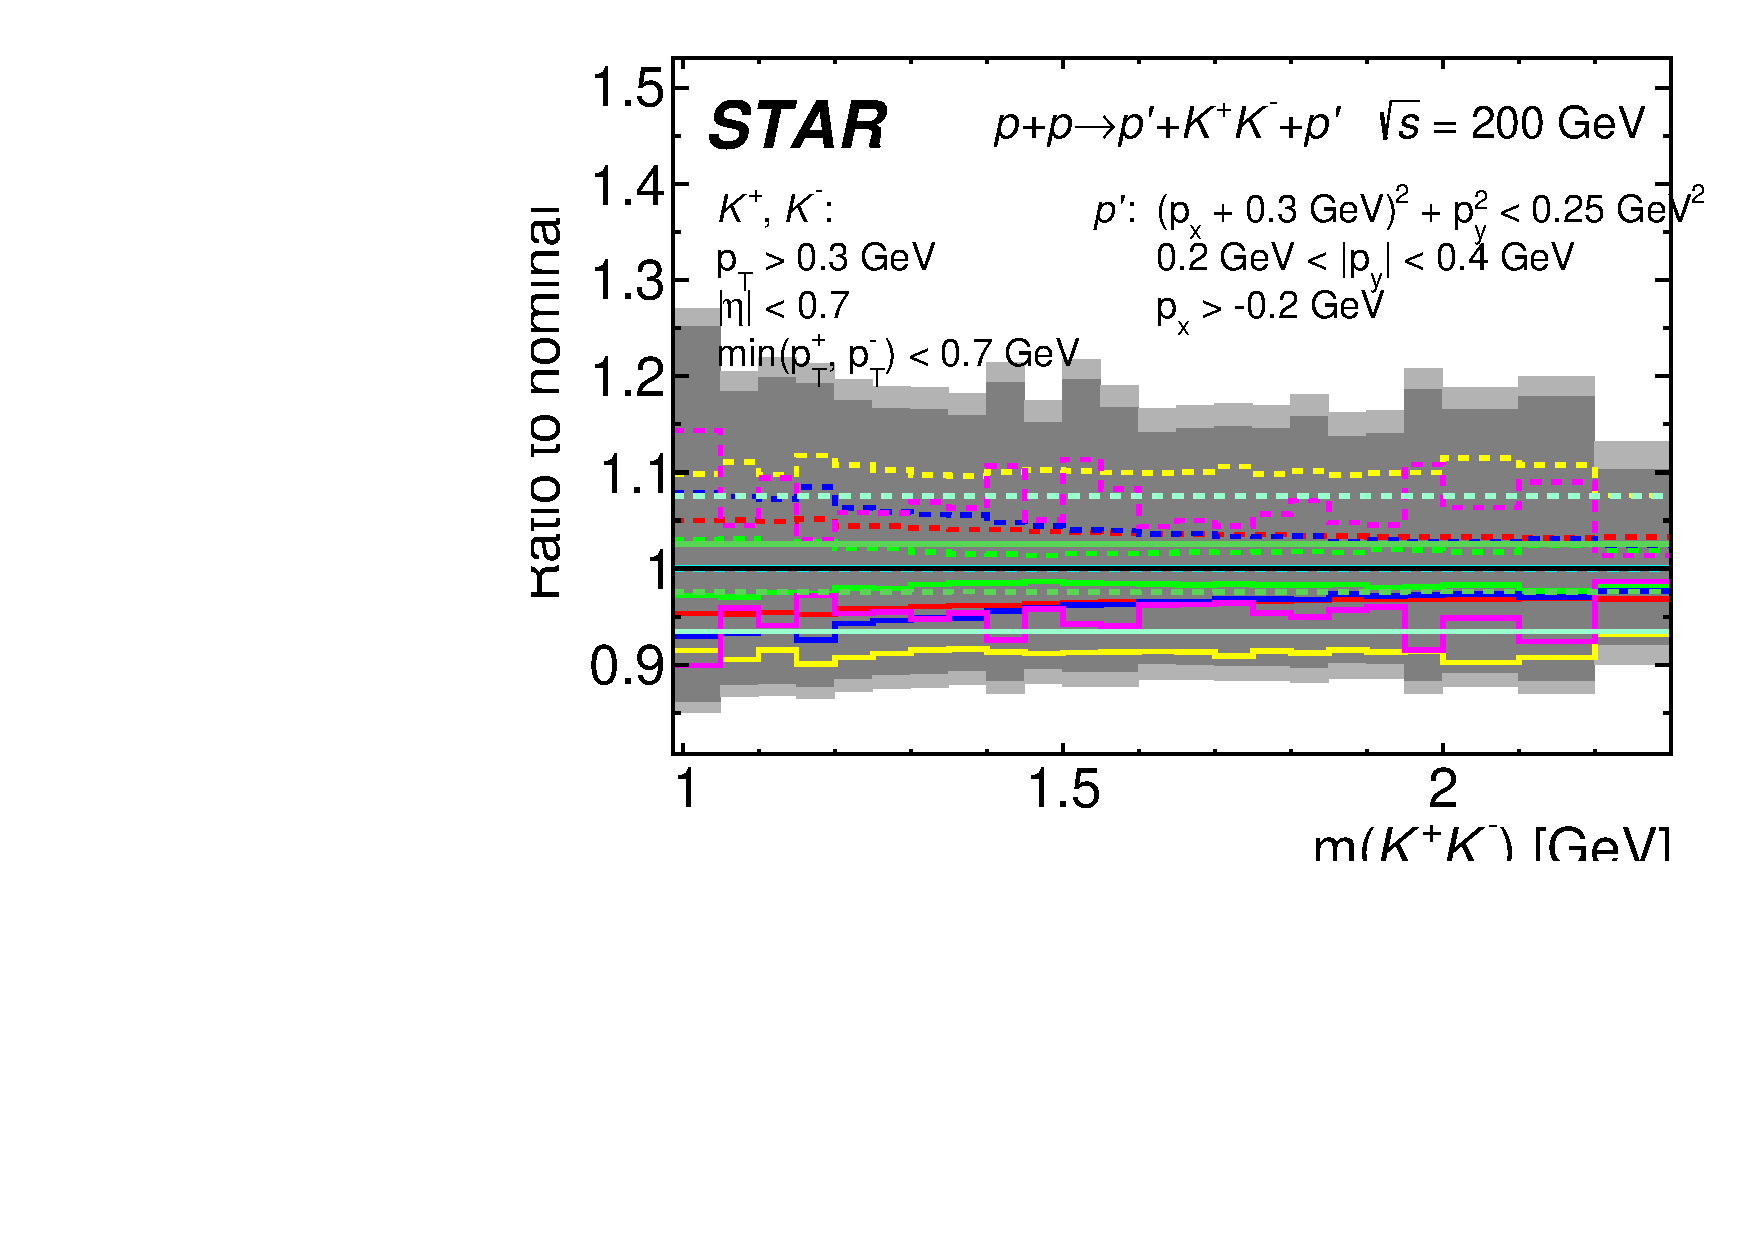
\includegraphics[width=.48\textwidth,page=1]{graphics/systematics/FinalResult_InvMass_kaon_Systematics2.pdf}
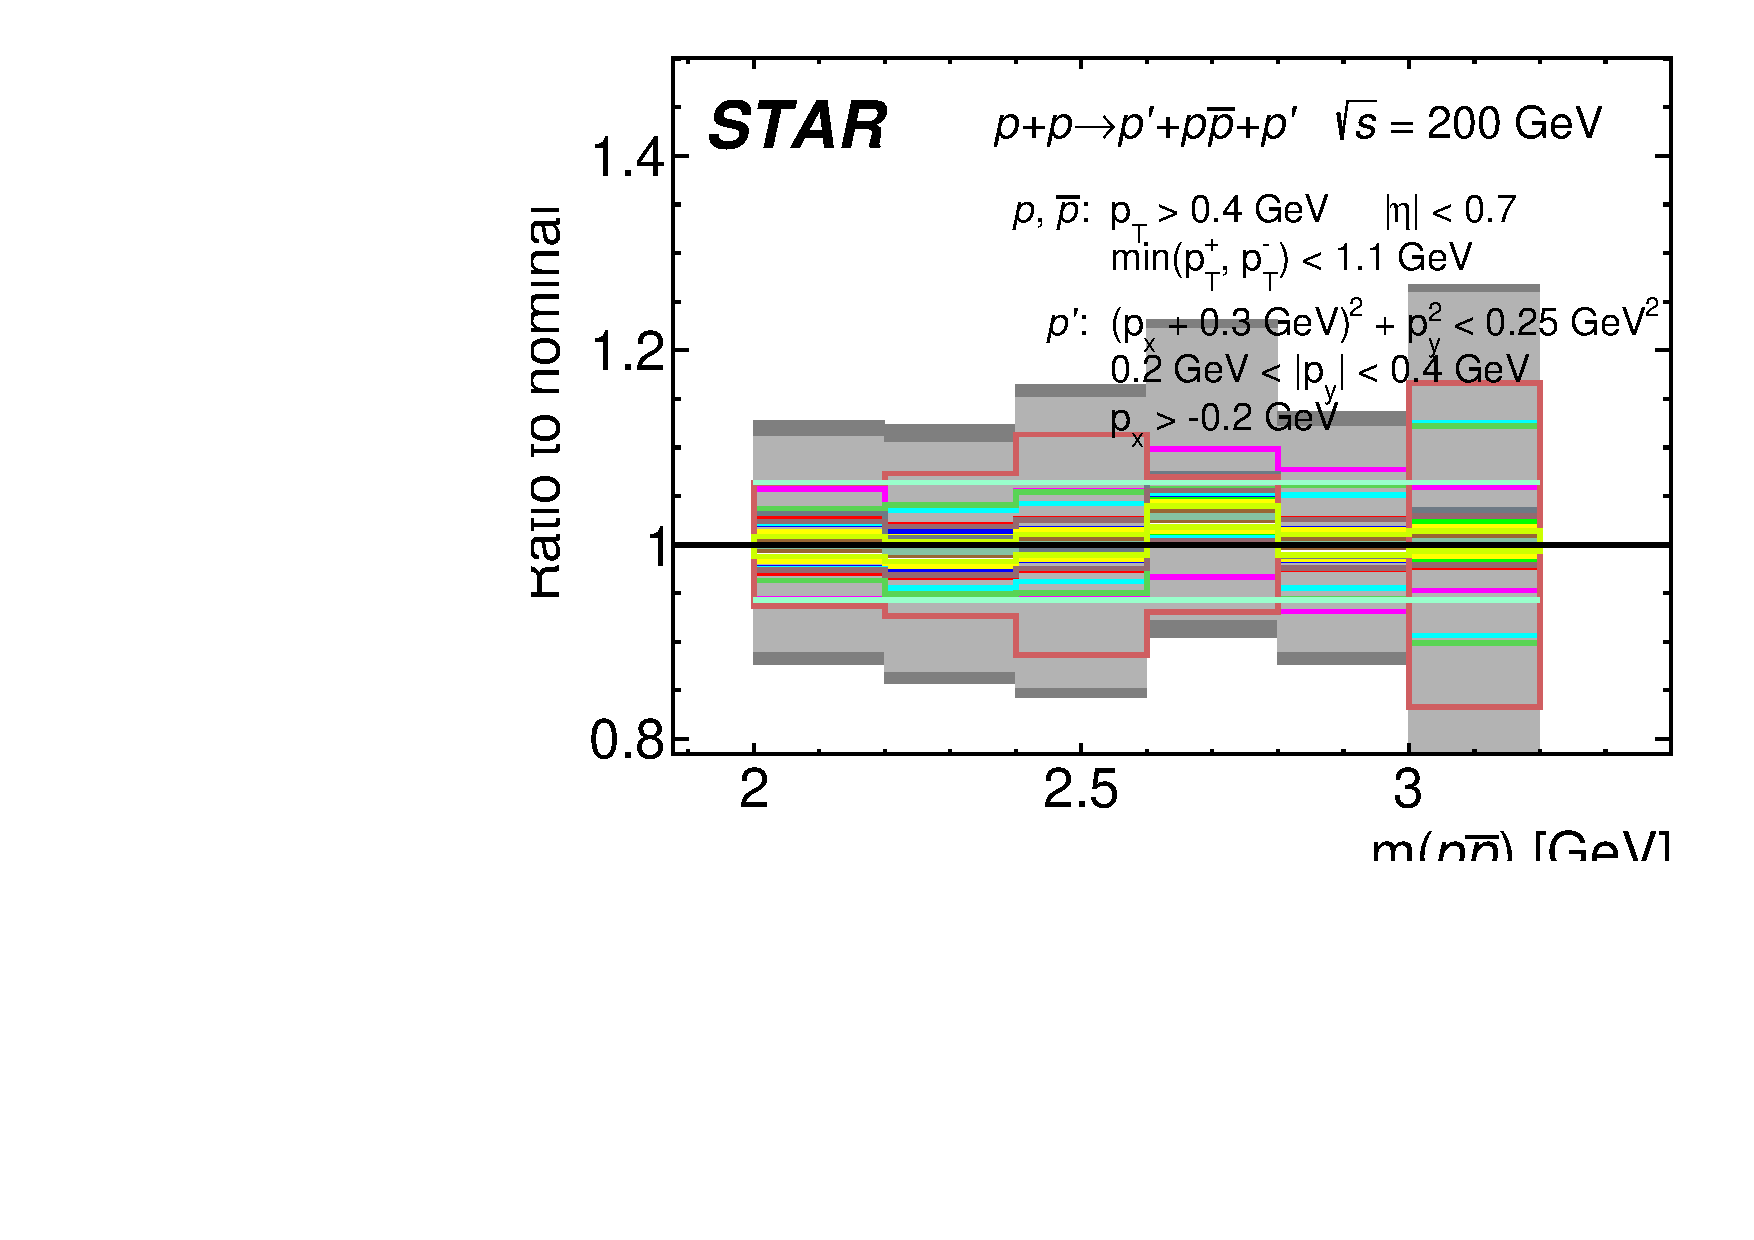
\includegraphics[width=.48\textwidth,page=1]{graphics/systematics/FinalResult_InvMass_proton_Systematics2.pdf}
%
\caption{Systematic uncertainties of the differential cross sections for CEP of charged particle pairs $K^+K^-$ (left) and $p\bar{p}$ (right) as a function of the invariant mass of the pair in the fiducial region explained on the plots.}
\label{systematics_02}
\end{figure}
% 
\begin{figure}[h]
\centering
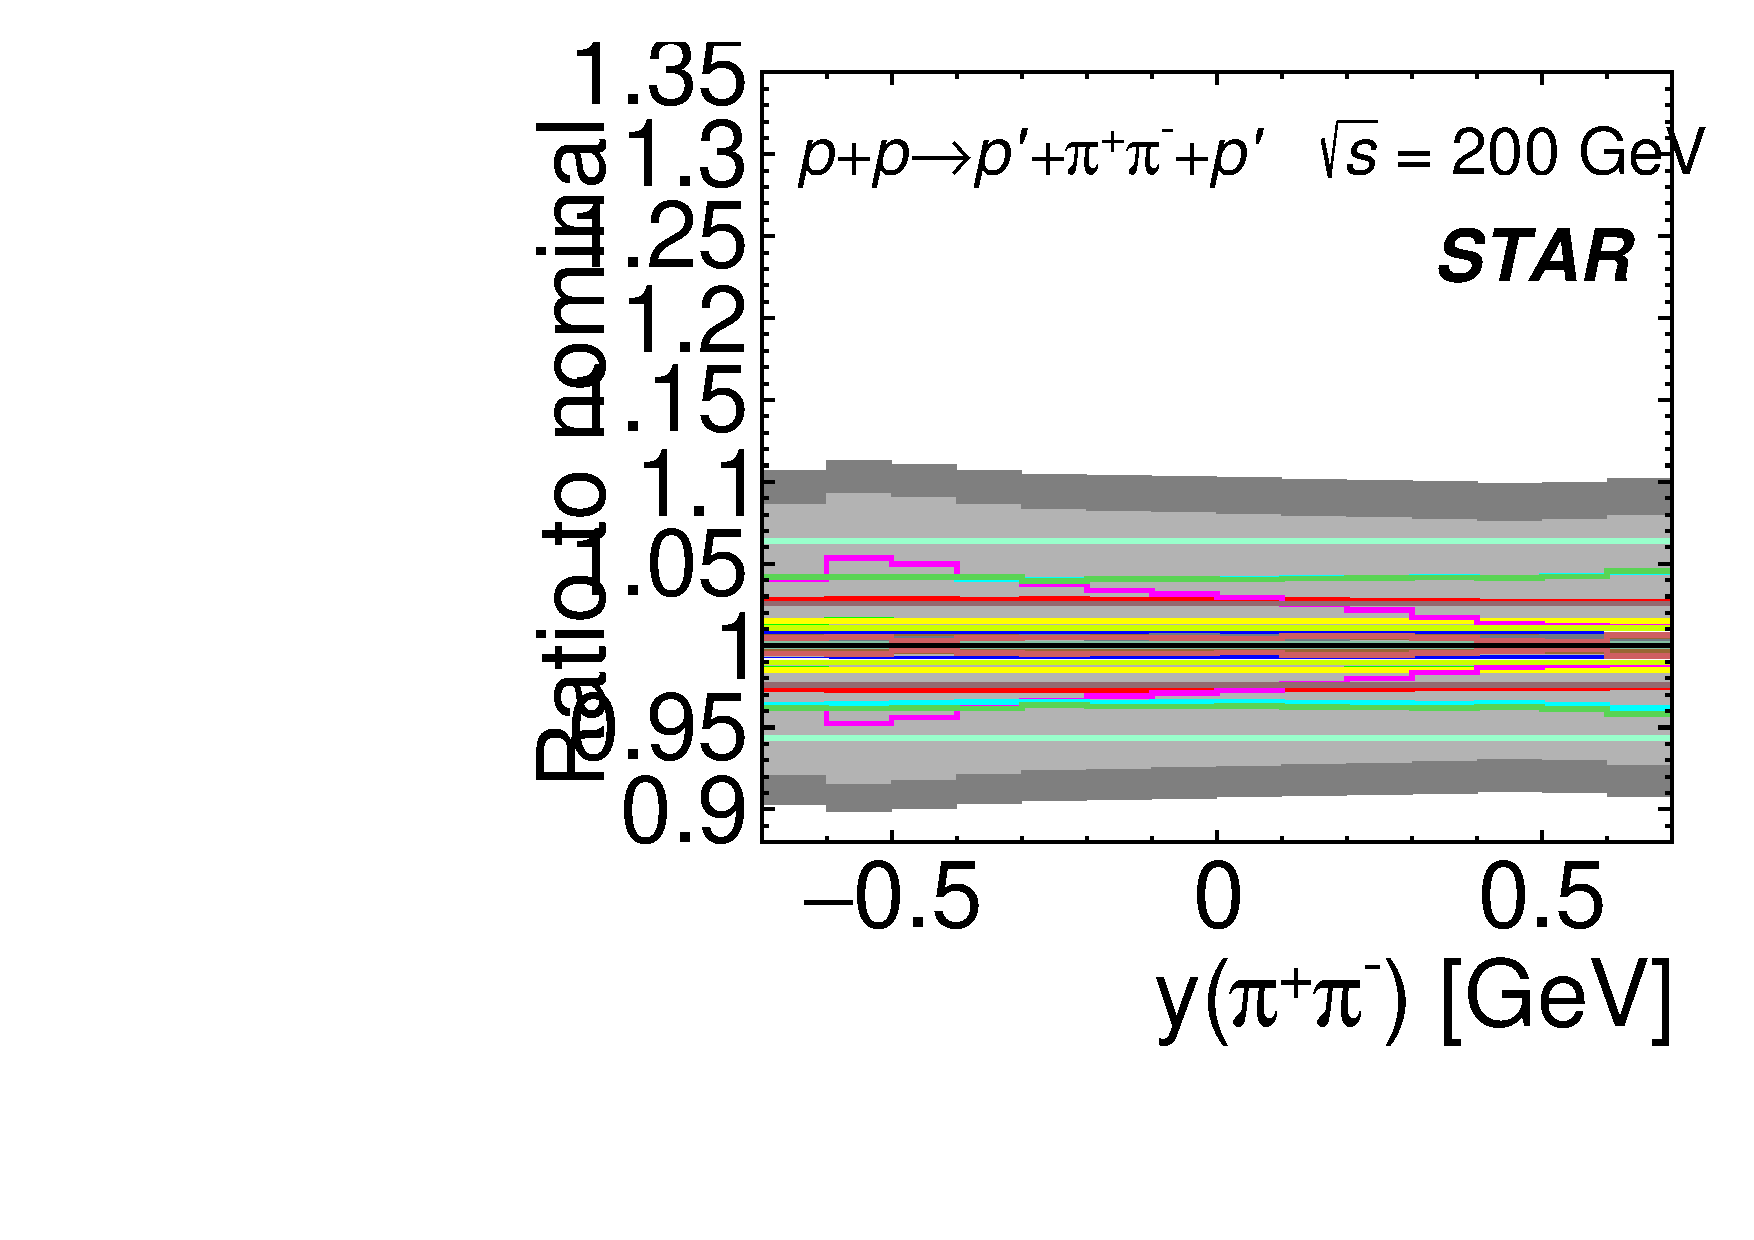
\includegraphics[width=.31\textwidth,page=1]{graphics/systematics/FinalResult_Rapidity_pion_Systematics2.pdf}
\hfill
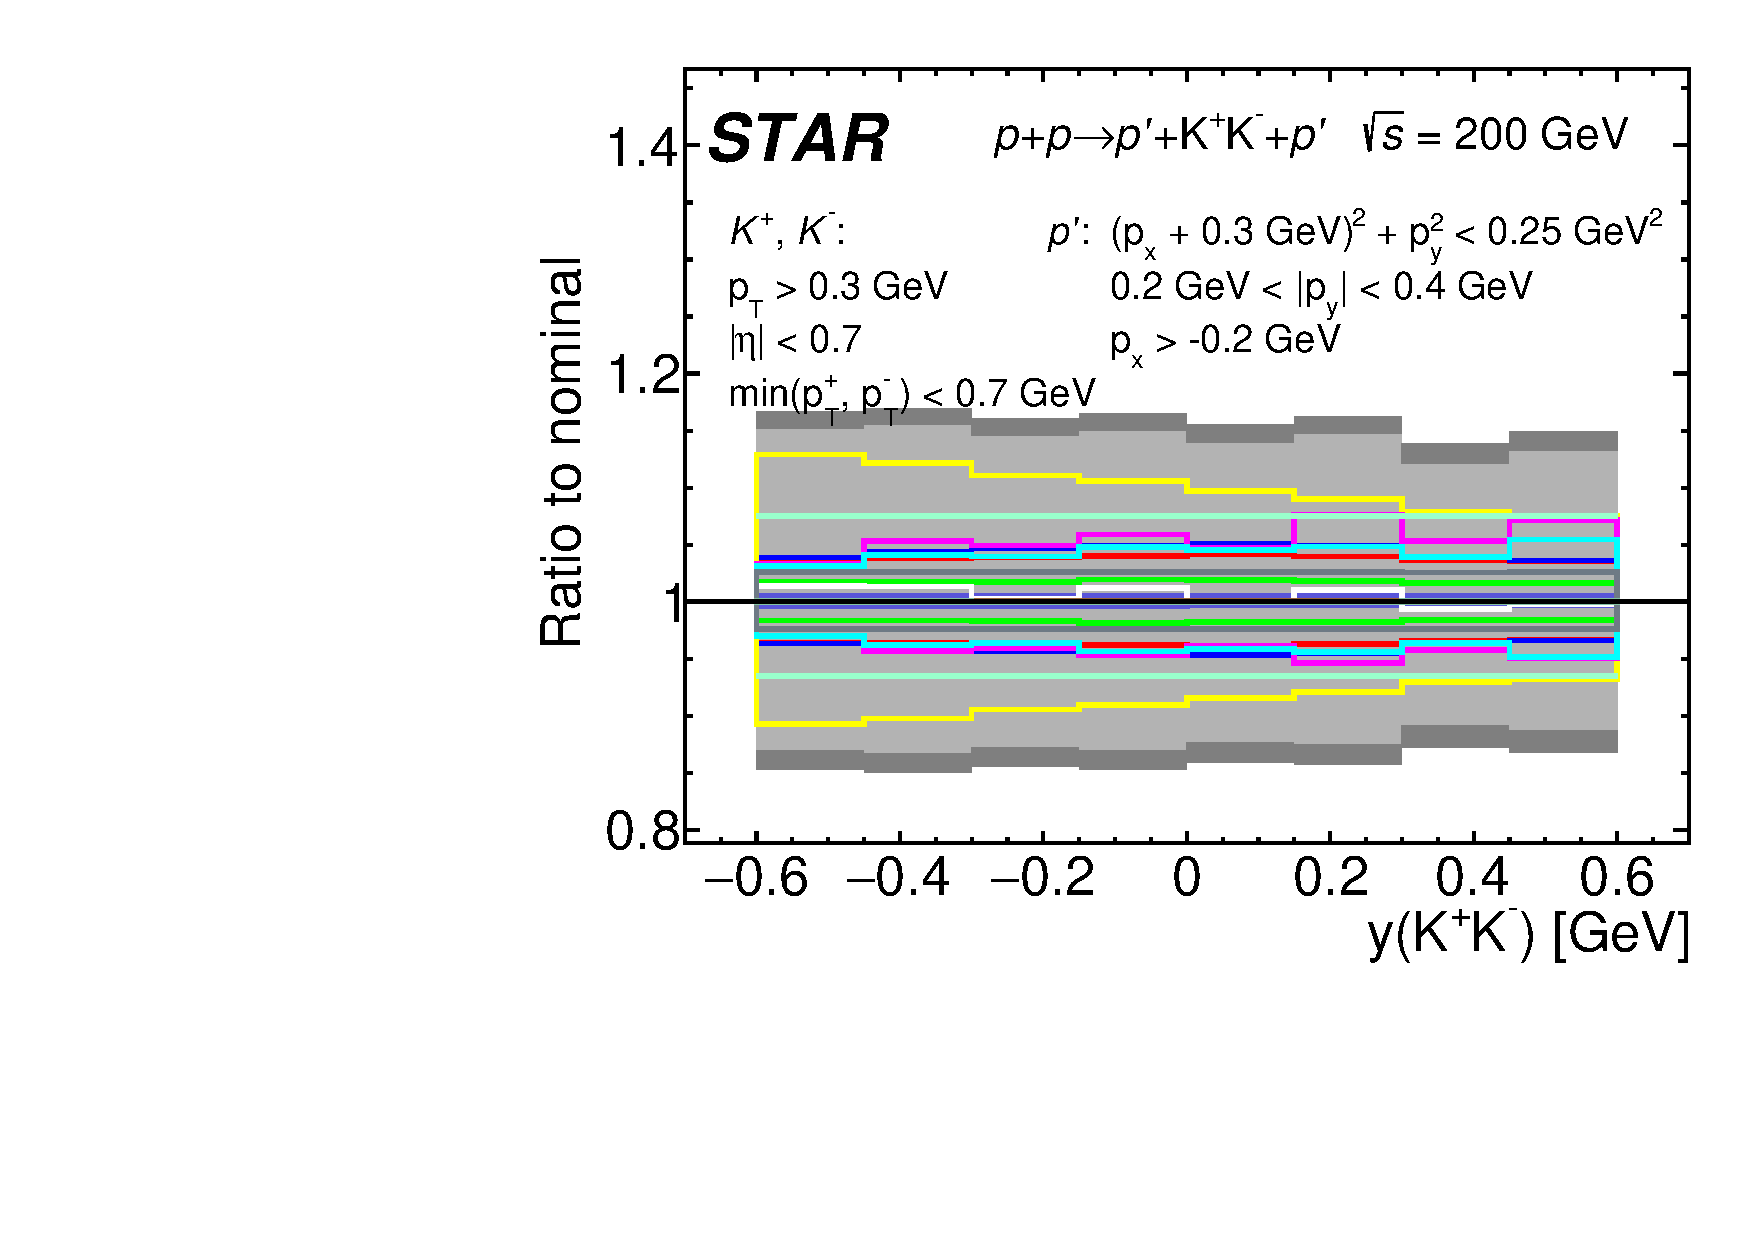
\includegraphics[width=.31\textwidth,page=1]{graphics/systematics/FinalResult_Rapidity_kaon_Systematics2.pdf}
\hfill
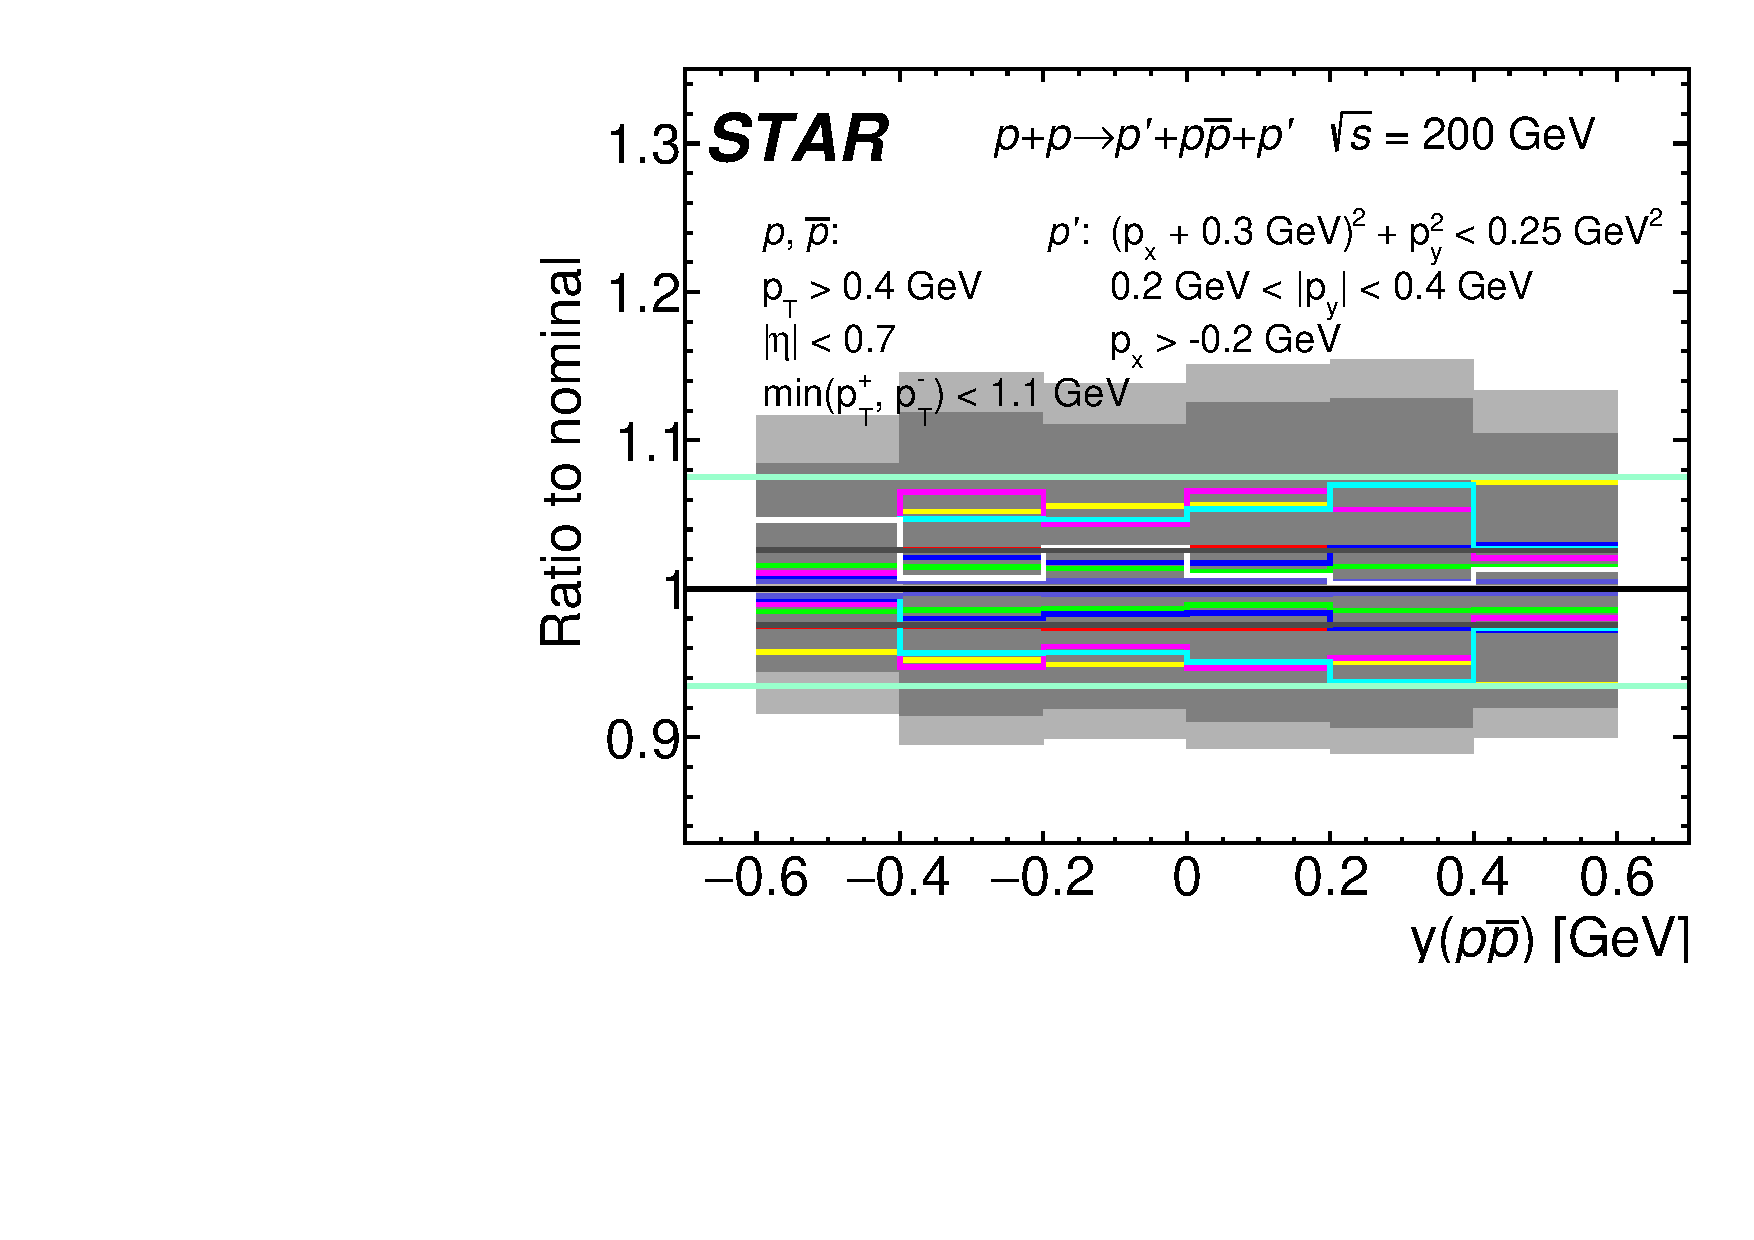
\includegraphics[width=.31\textwidth,page=1]{graphics/systematics/FinalResult_Rapidity_proton_Systematics2.pdf}
%
\caption{Systematic uncertainties of the differential cross sections for CEP of charged particle pairs $\pi^+\pi^-$ (let), $K^+K^-$ (middle) and $p\bar{p}$ (right) as a function of the pair rapidity measured in the fiducial region explained on the plots.}
\label{systematics_1}
\end{figure}
%
% \indent
% Figure~\ref{systematics_2}(right column) shows the differential cross sections for CEP of different particle species pairs as a function of the sum of the squares of the four-momenta transfers at the proton vertices.
% %
% The shapes of measured cross sections are strongly affected by the fiducial cuts applied to the forward scattered protons.
% %
% The shapes of the differential cross sections for both $\pi^+\pi^-$ snd $K^+K^-$ pairs production are better described by the DiMe model than by GenEx and MBR models.
% In case of the cross section for $p\bar{p}$ pairs production the MBR model implemented in PYTHIA8 describes normalization of the data fairly well but predicts a steeper slope.\\
% %
% \indent
% Figure~\ref{systematics_3} shows the differential cross sections for CEP of different particle species pairs as a function of the pair invariant mass separately in two $\Delta\phi$ regions: $\Delta\phi<90$ degree (left column) and $\Delta\phi>90$ degree (right column).
% %
% Sharp drops of the measured cross sections at $m(\pi^+\pi^-) < 0.6$~GeV and at $m(K^+K^-) < 1.3$~GeV for the $\Delta\phi>$ 90 degree range are due to the fiducial cuts applied to the forward scattered protons. 
% %
% In case of the cross section for CEP of $\pi^+\pi^-$ pairs in $\Delta\phi<90$ degree range the peak around $f_2(1270)$ resonance in data is significantly suppressed while the peak at $f_0(980)$ is enhanced as well as possible resonances in the mass range $1.3-1.5$ MeV compared to the $\Delta\phi>90$ degrees range. 
%
\begin{figure}[h]
\centering
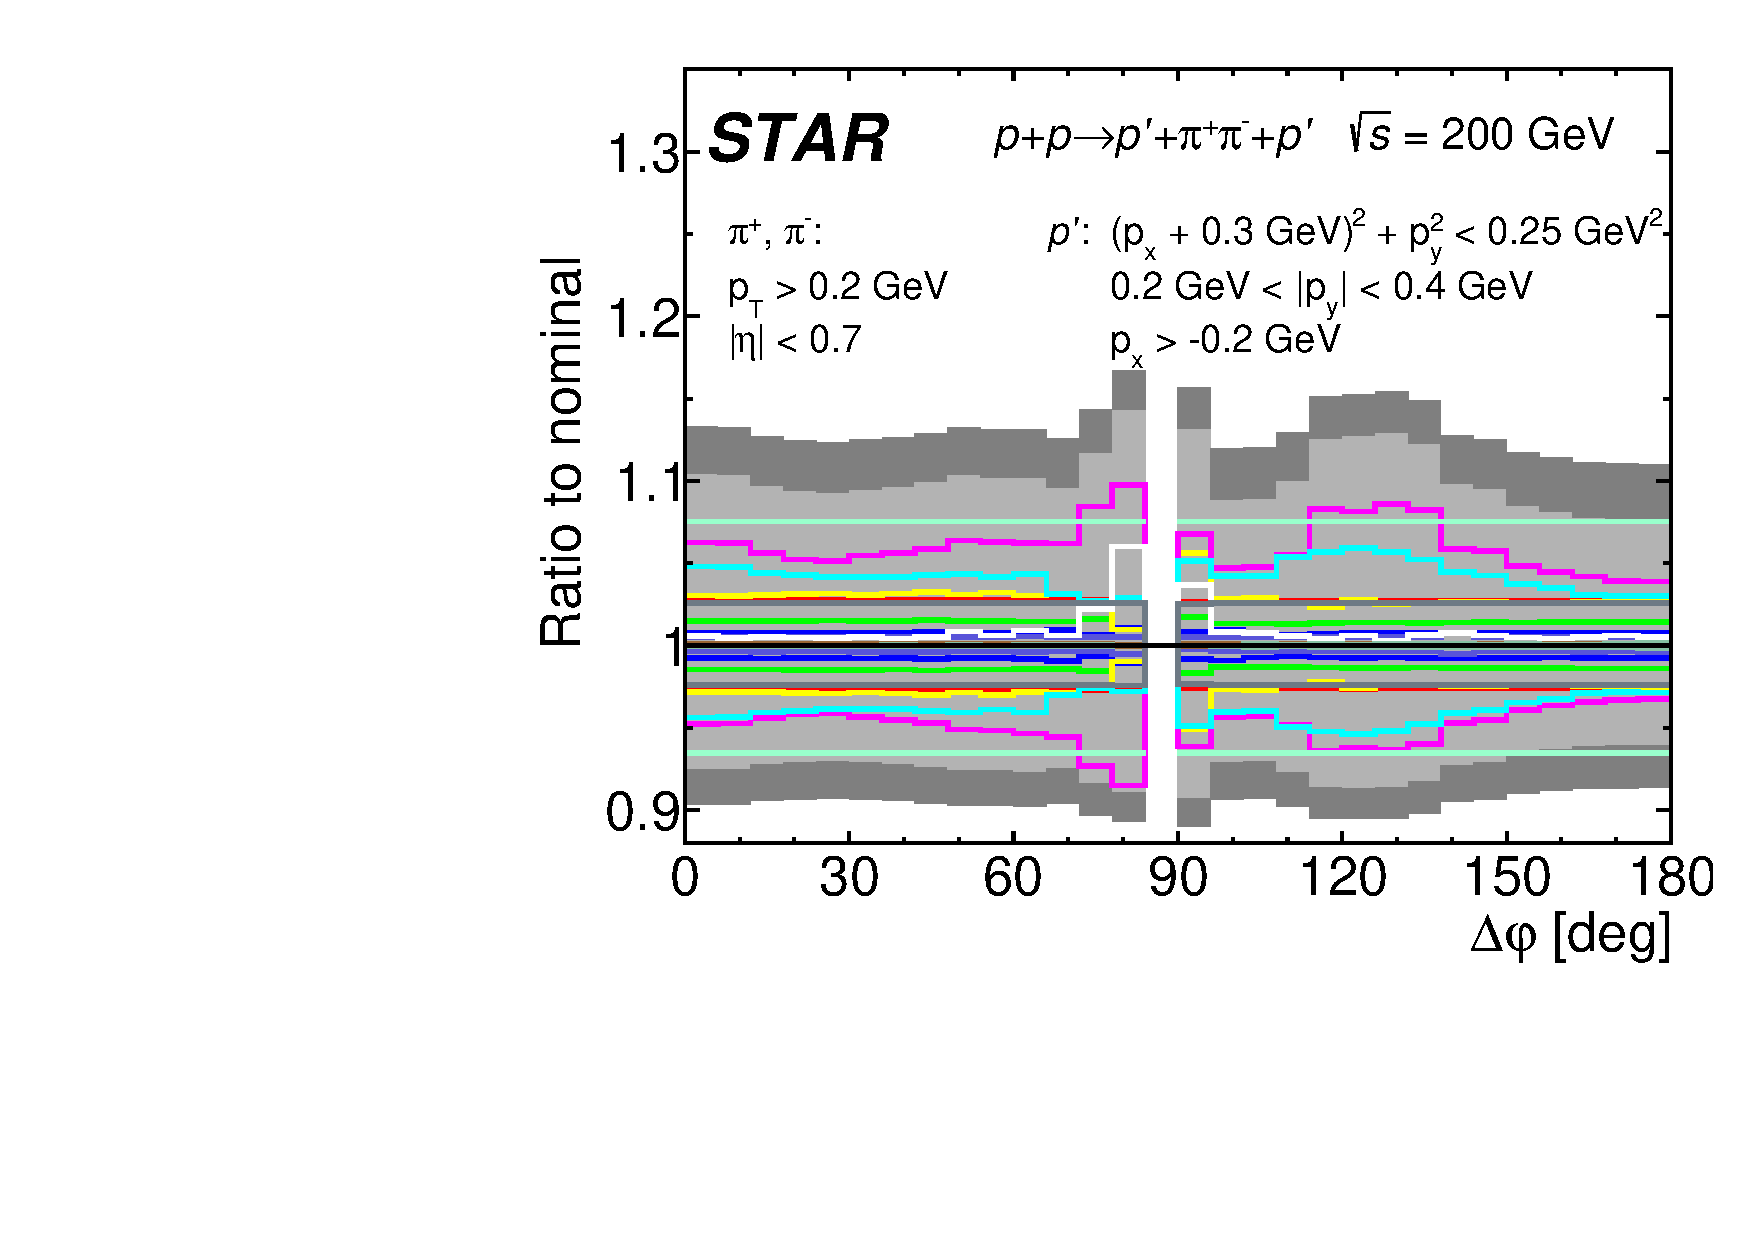
\includegraphics[width=.31\textwidth,page=1]{graphics/systematics/FinalResult_DeltaPhi_pion_Systematics2.pdf}
\hfill
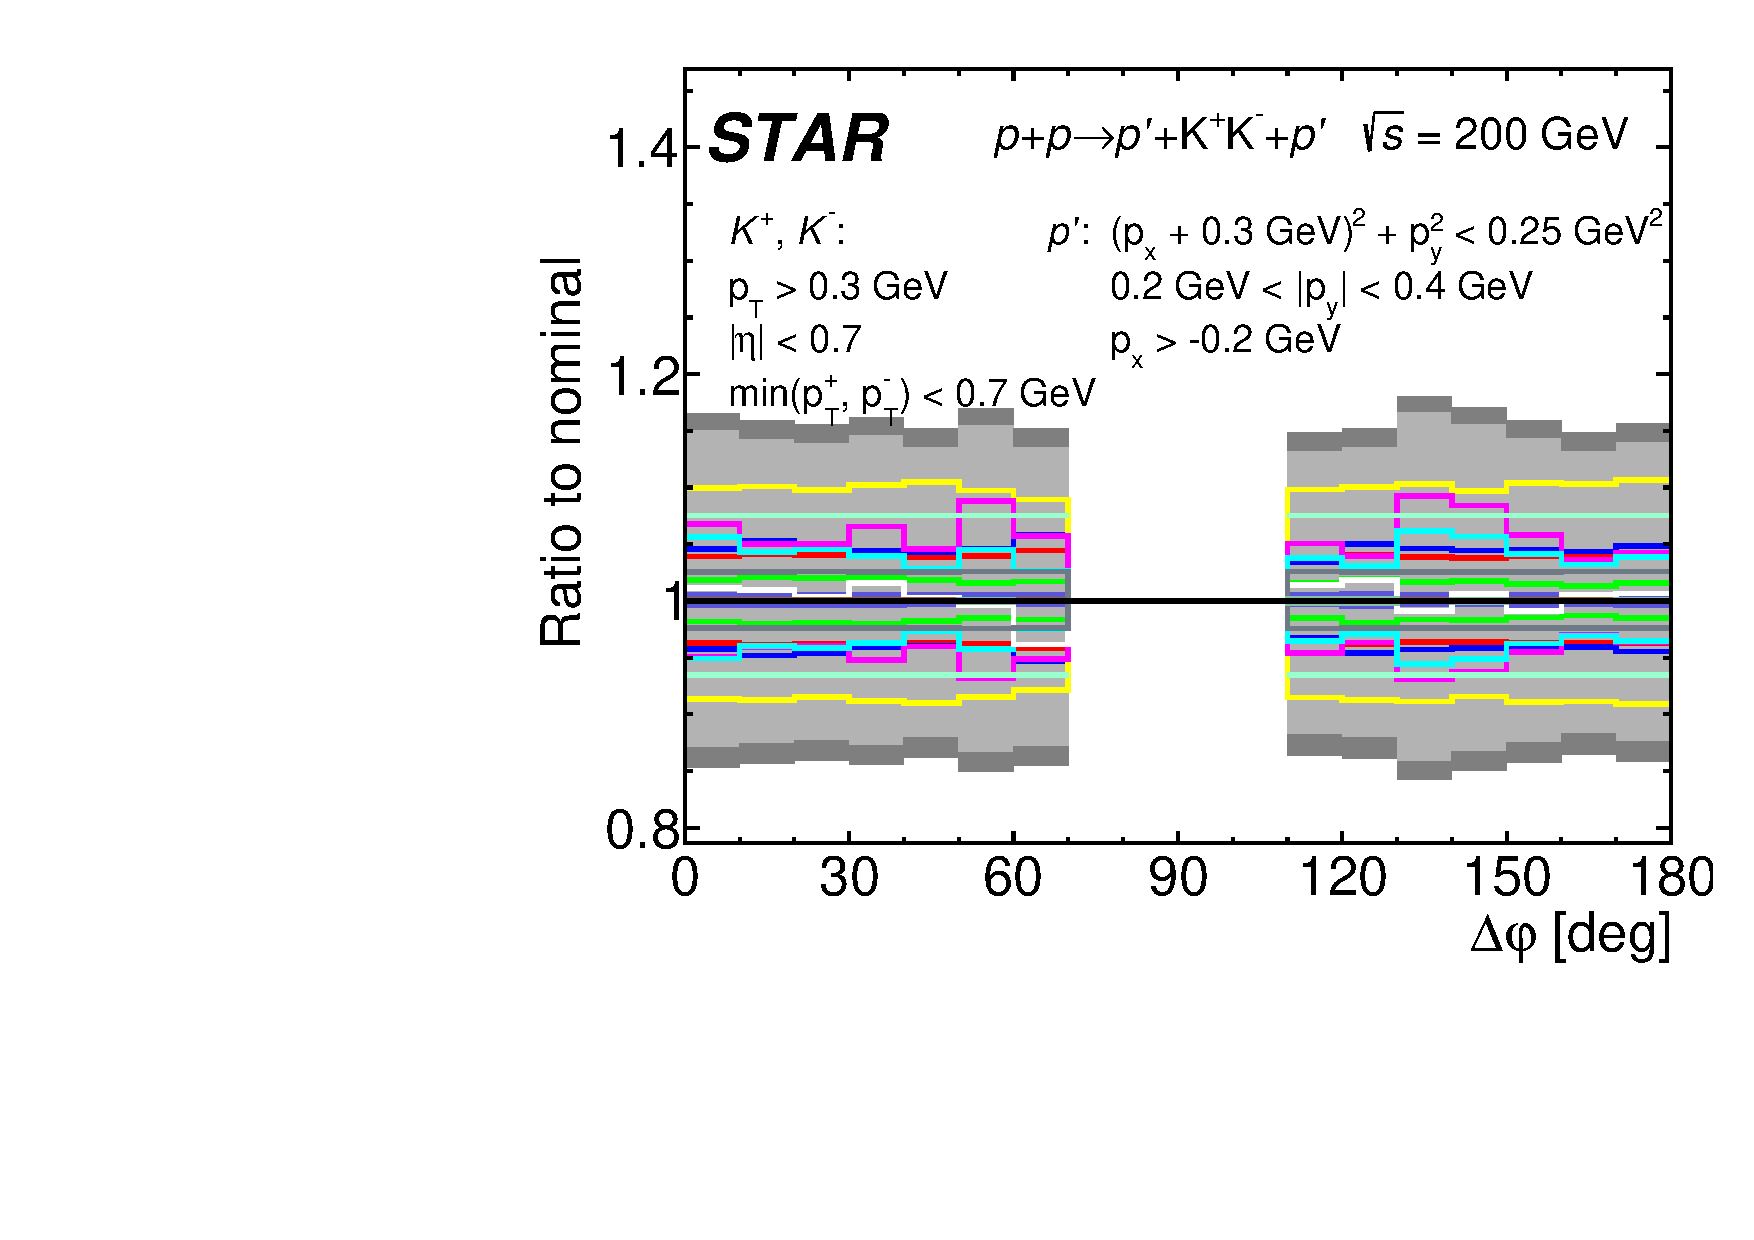
\includegraphics[width=.31\textwidth,page=1]{graphics/systematics/FinalResult_DeltaPhi_kaon_Systematics2.pdf}
\hfill
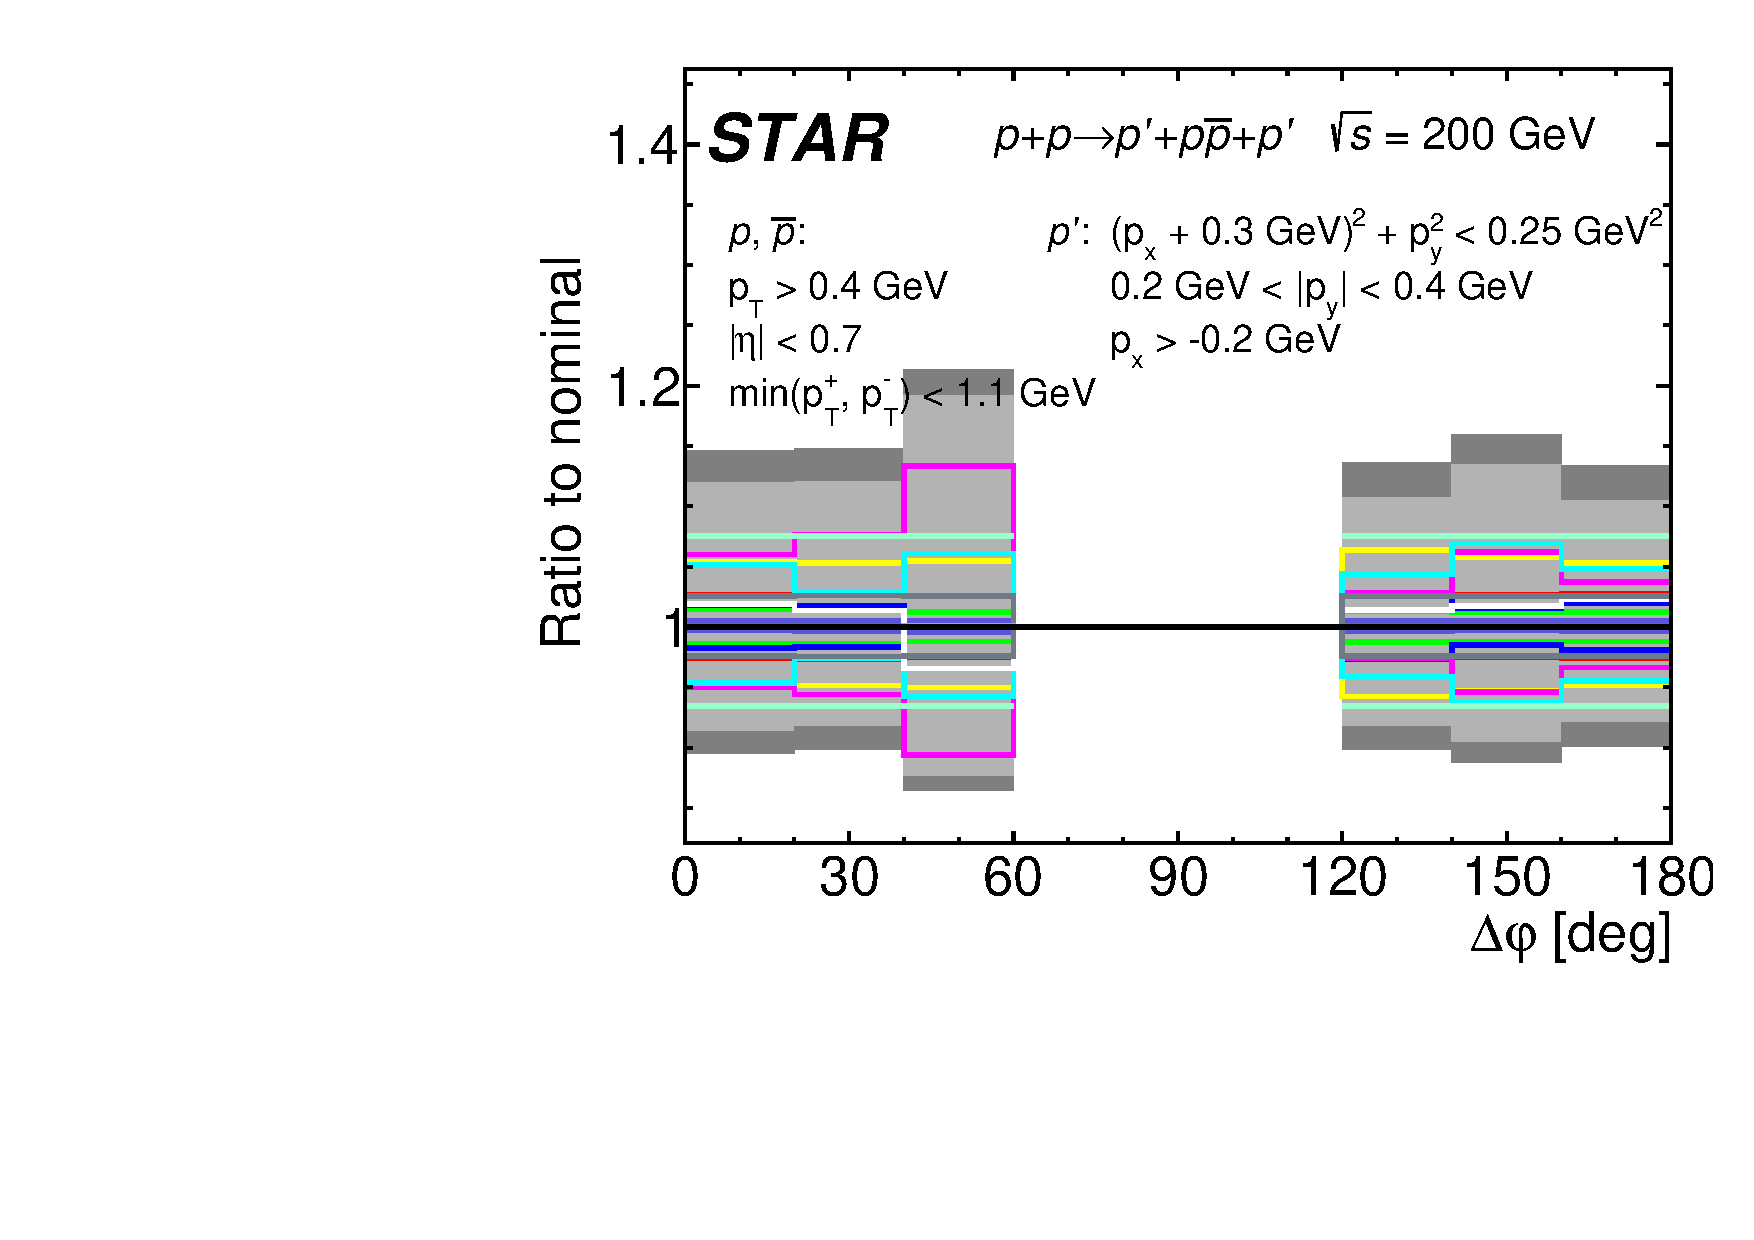
\includegraphics[width=.31\textwidth,page=1]{graphics/systematics/FinalResult_DeltaPhi_proton_Systematics2.pdf}
\newline
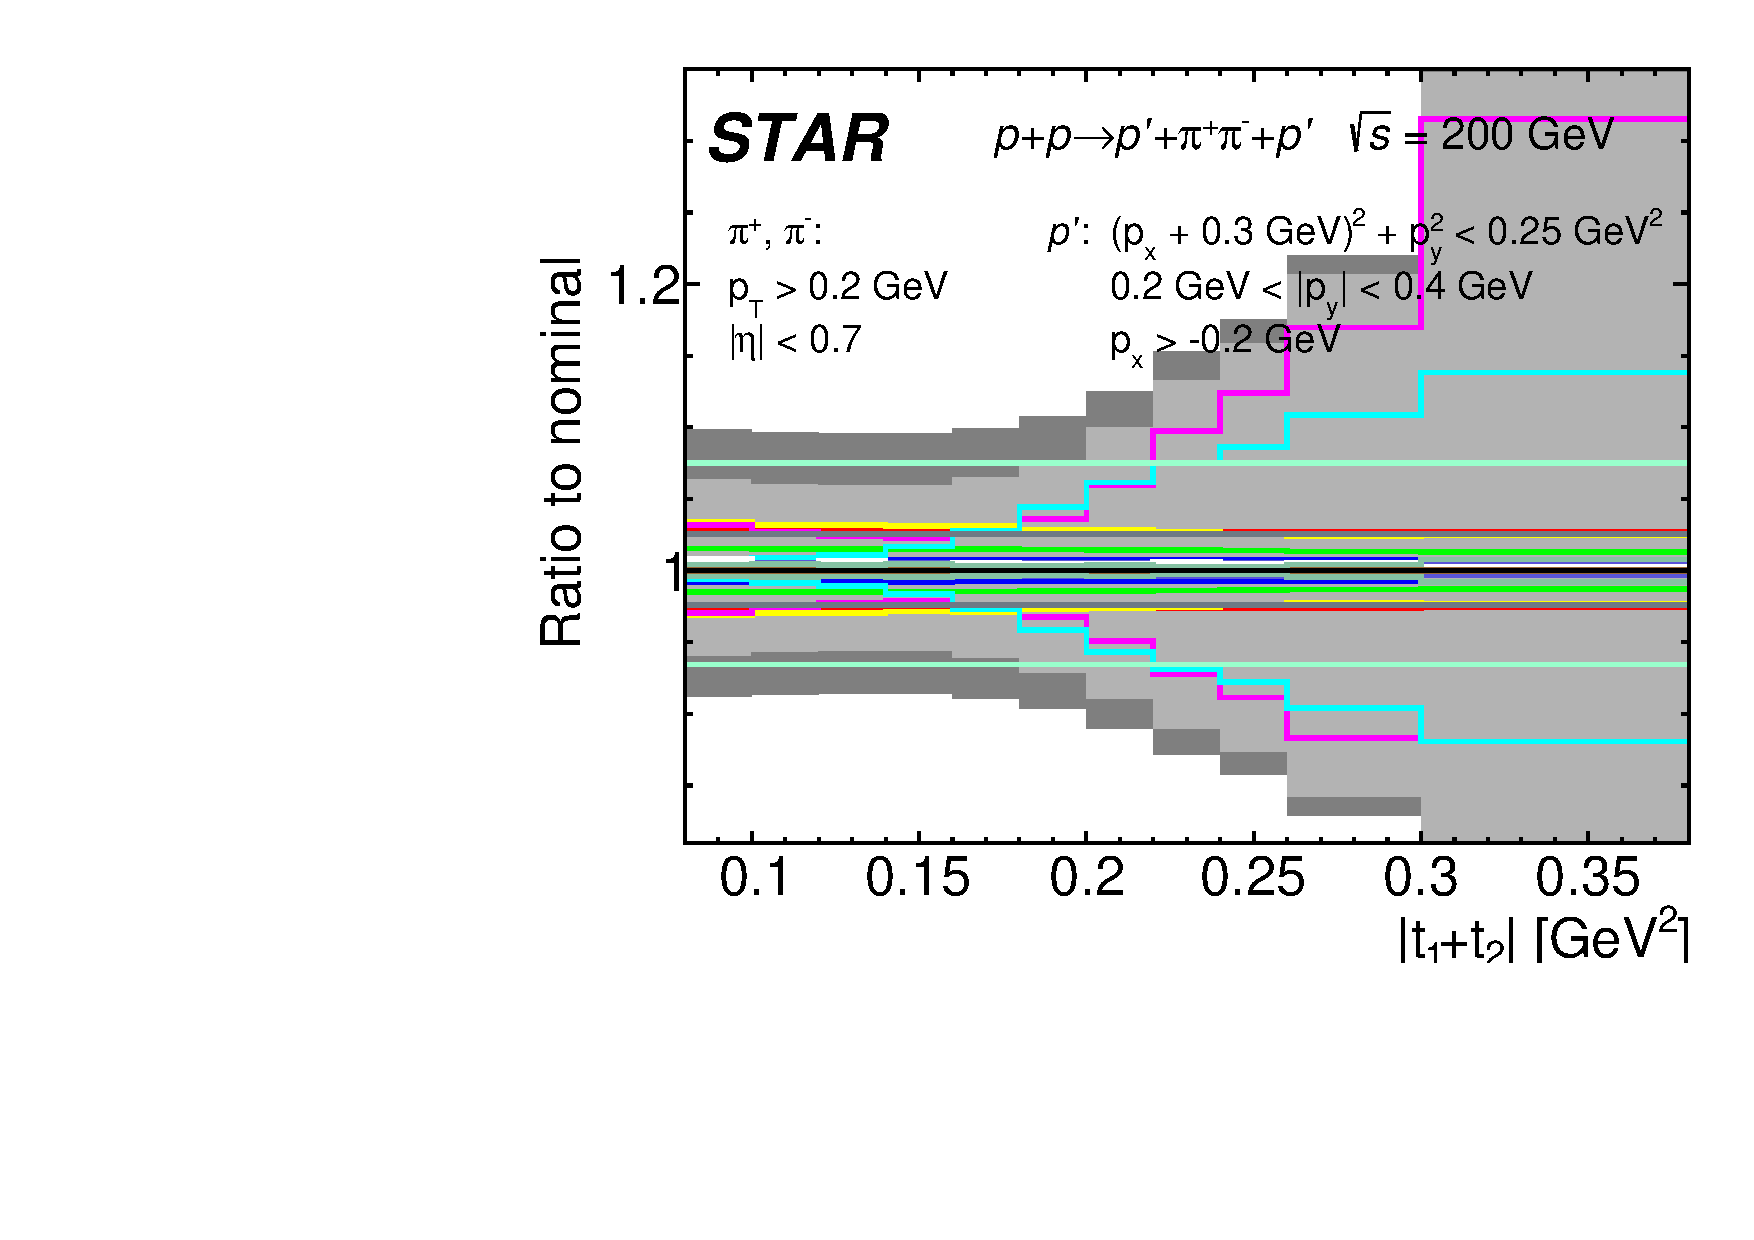
\includegraphics[width=.31\textwidth,page=1]{graphics/systematics/FinalResult_MandelstamTSum_pion_Systematics2.pdf}
\hfill
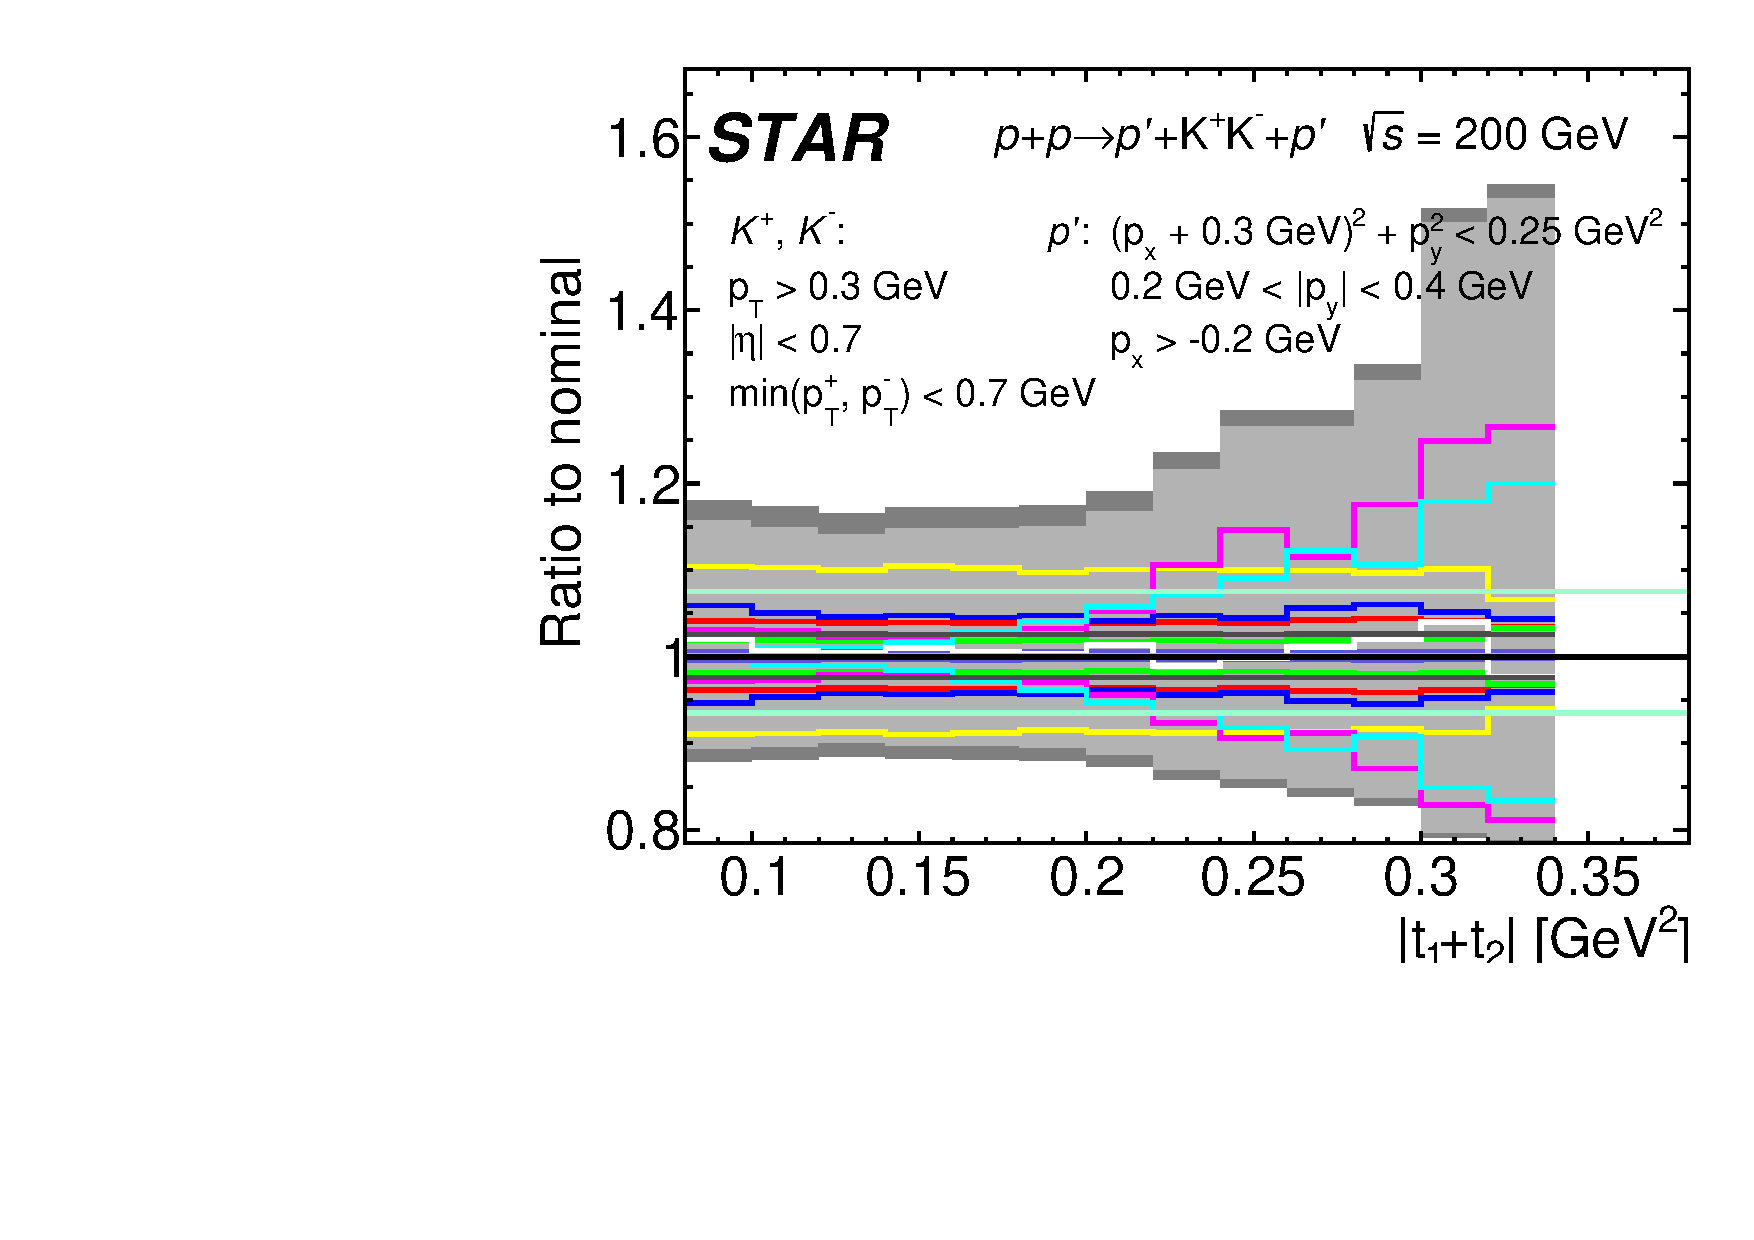
\includegraphics[width=.31\textwidth,page=1]{graphics/systematics/FinalResult_MandelstamTSum_kaon_Systematics2.pdf}
\hfill
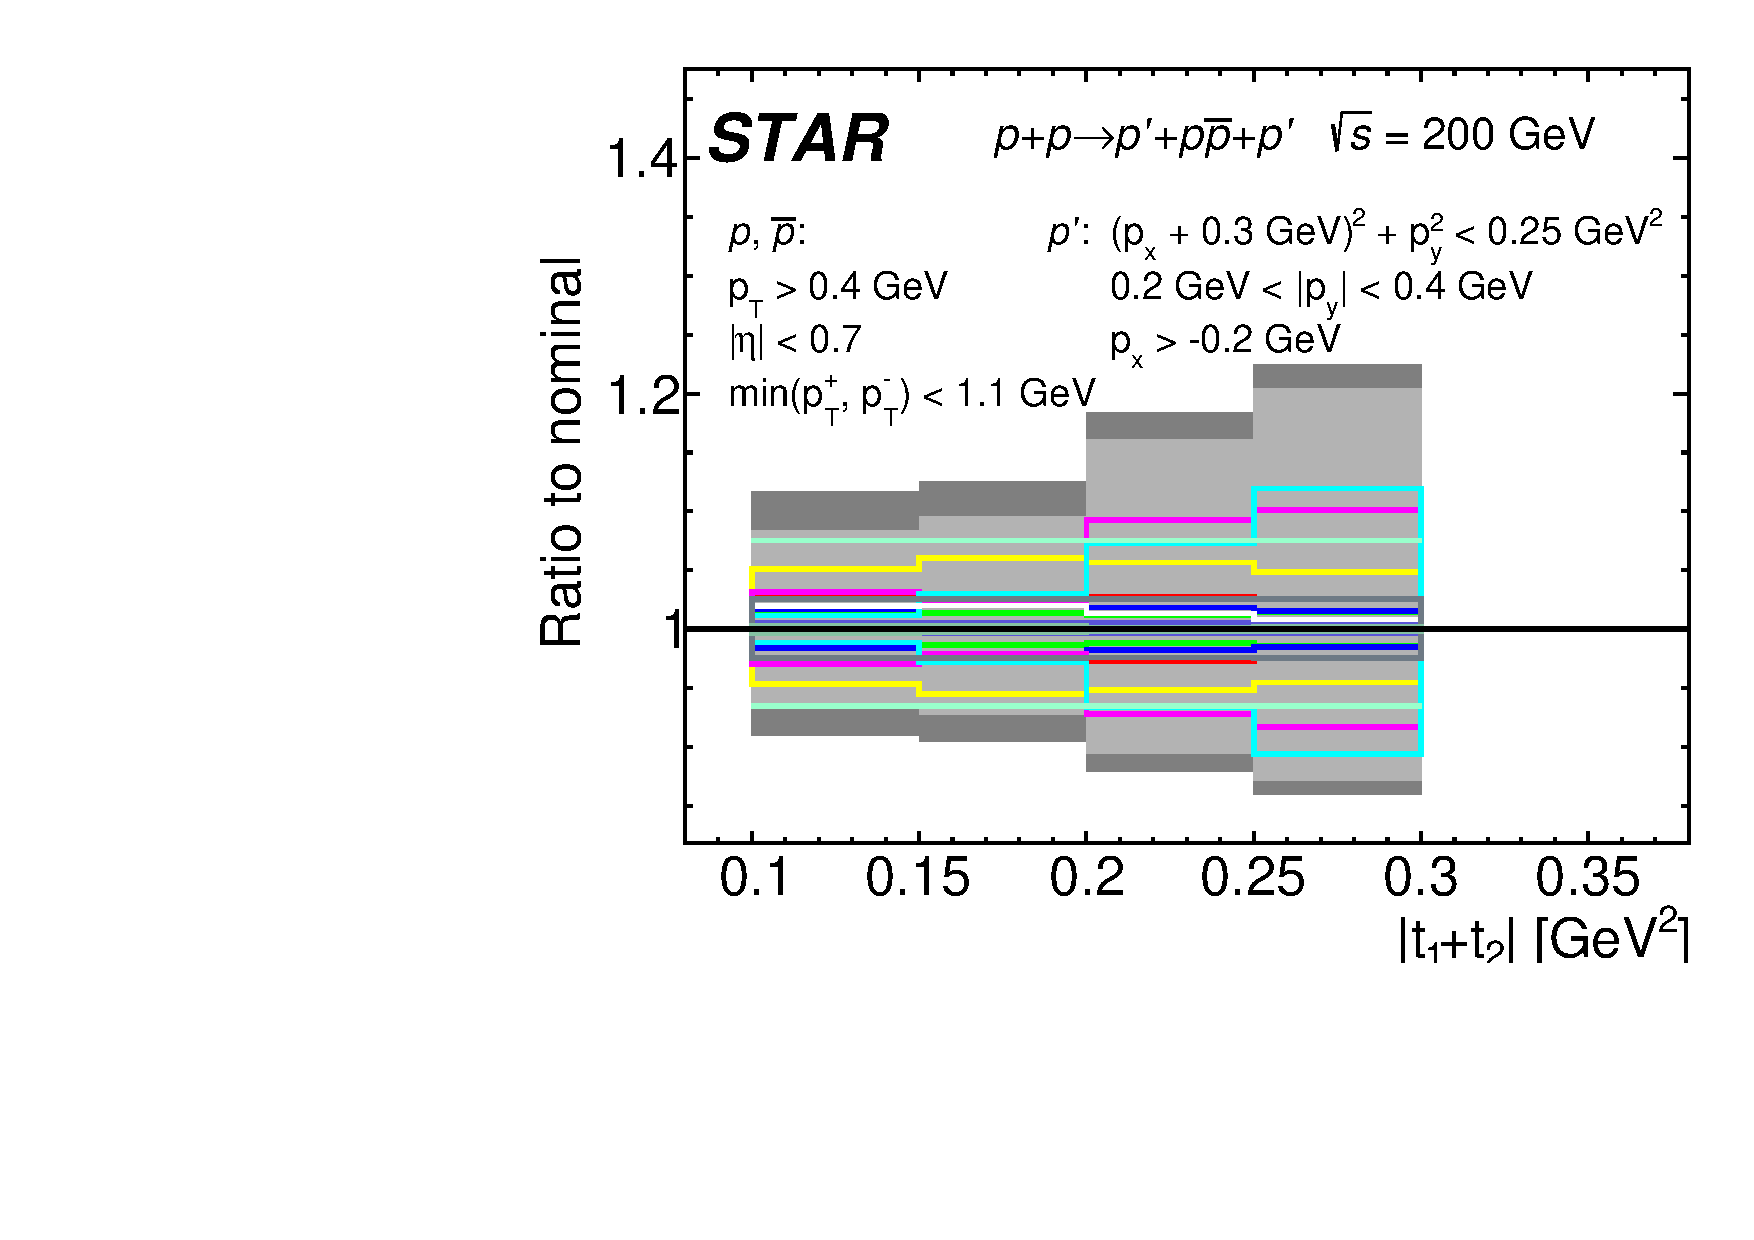
\includegraphics[width=.31\textwidth,page=1]{graphics/systematics/FinalResult_MandelstamTSum_proton_Systematics2.pdf}
%
\caption{Systematic uncertainties of the differential cross sections for CEP of charged particle pairs $\pi^+\pi^-$ (left column), $K^+K^-$ (middle column) and $p\bar{p}$ (right column) as a function of the difference of azimuthal angles of the forward scattered protons (top) and of the sum of the squares of the four-momenta losses in the proton vertices (bottom) measured in the fiducial region explained on the plots.}
\label{systematics_2}
\end{figure}
%
\begin{figure}[h]
\centering
\hspace*{5pt}
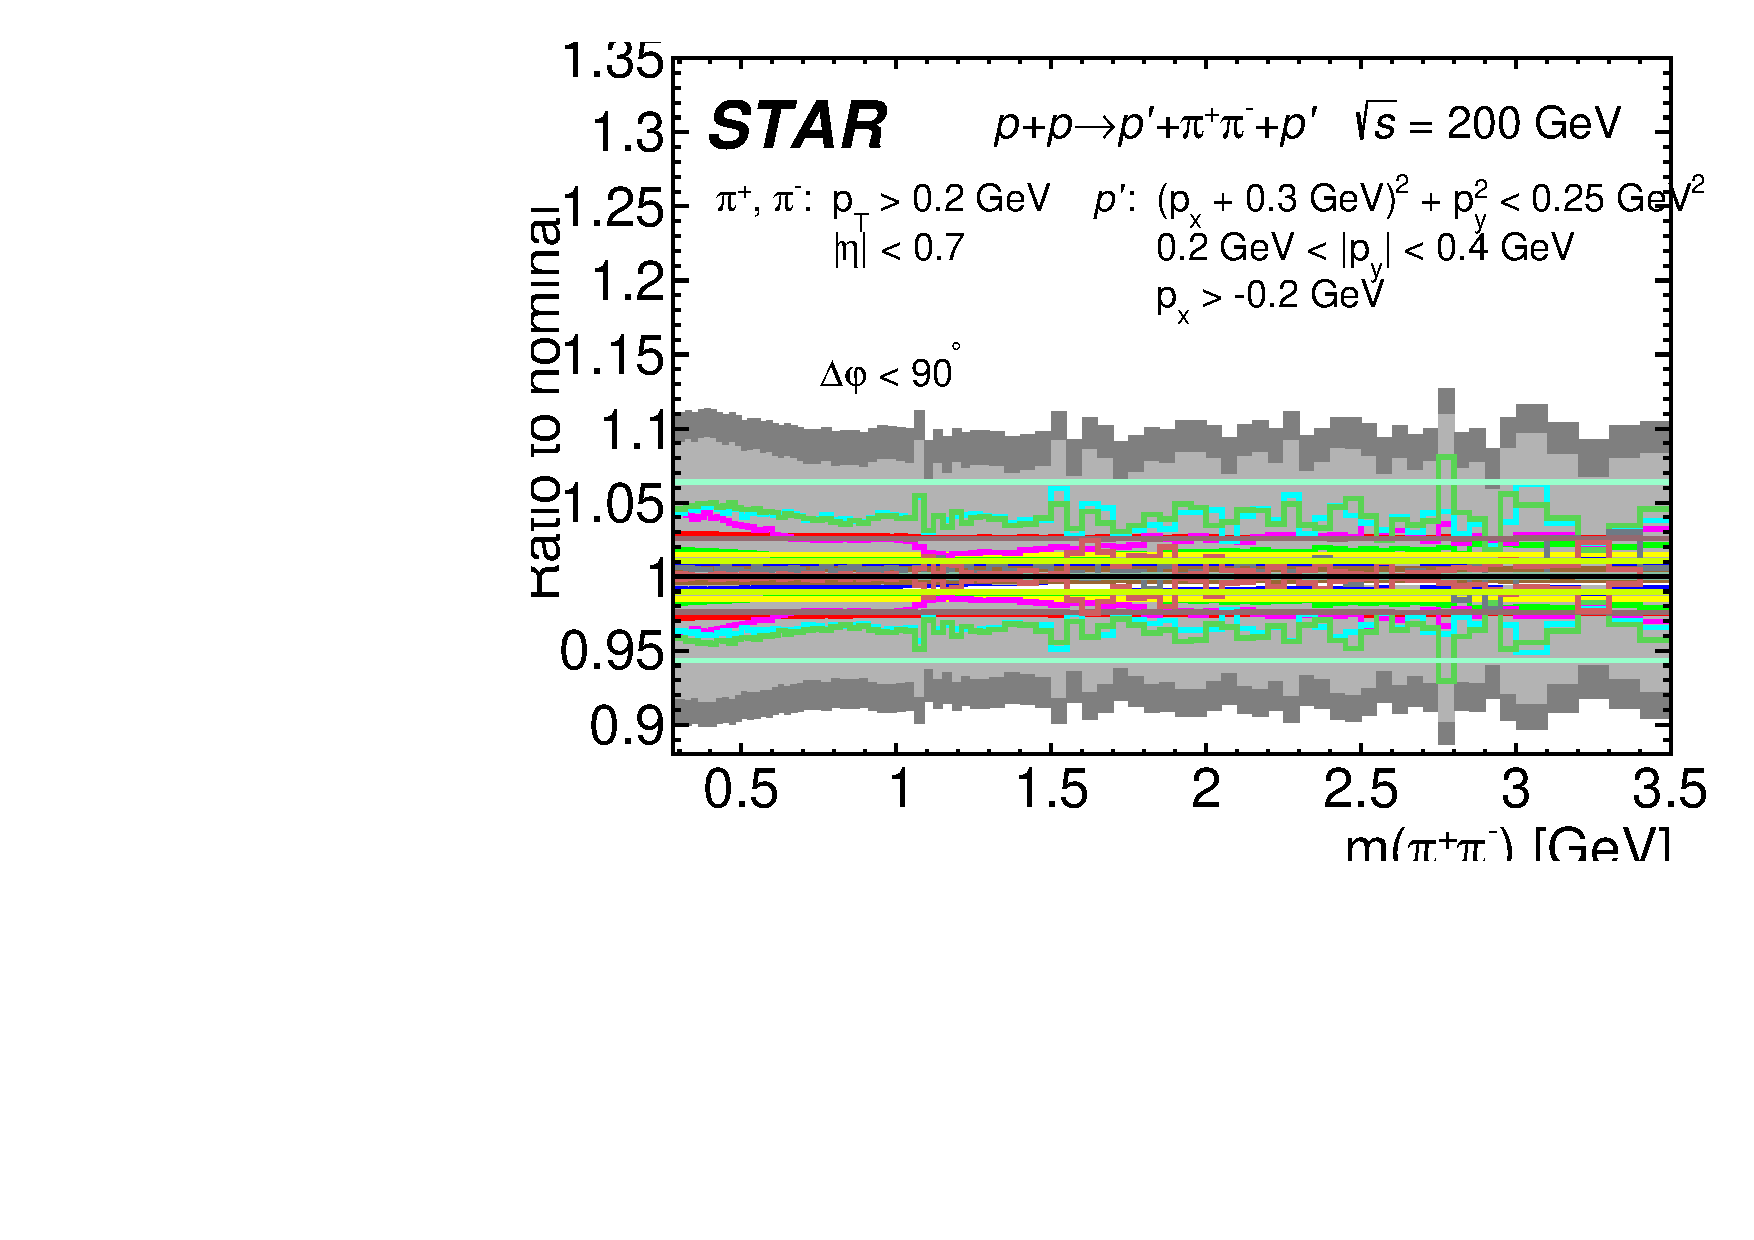
\includegraphics[width=.46\textwidth,page=1]{graphics/systematics/FinalResult_InvMass_DeltaPhiBin1_pion_Systematics2.pdf}
\hfill
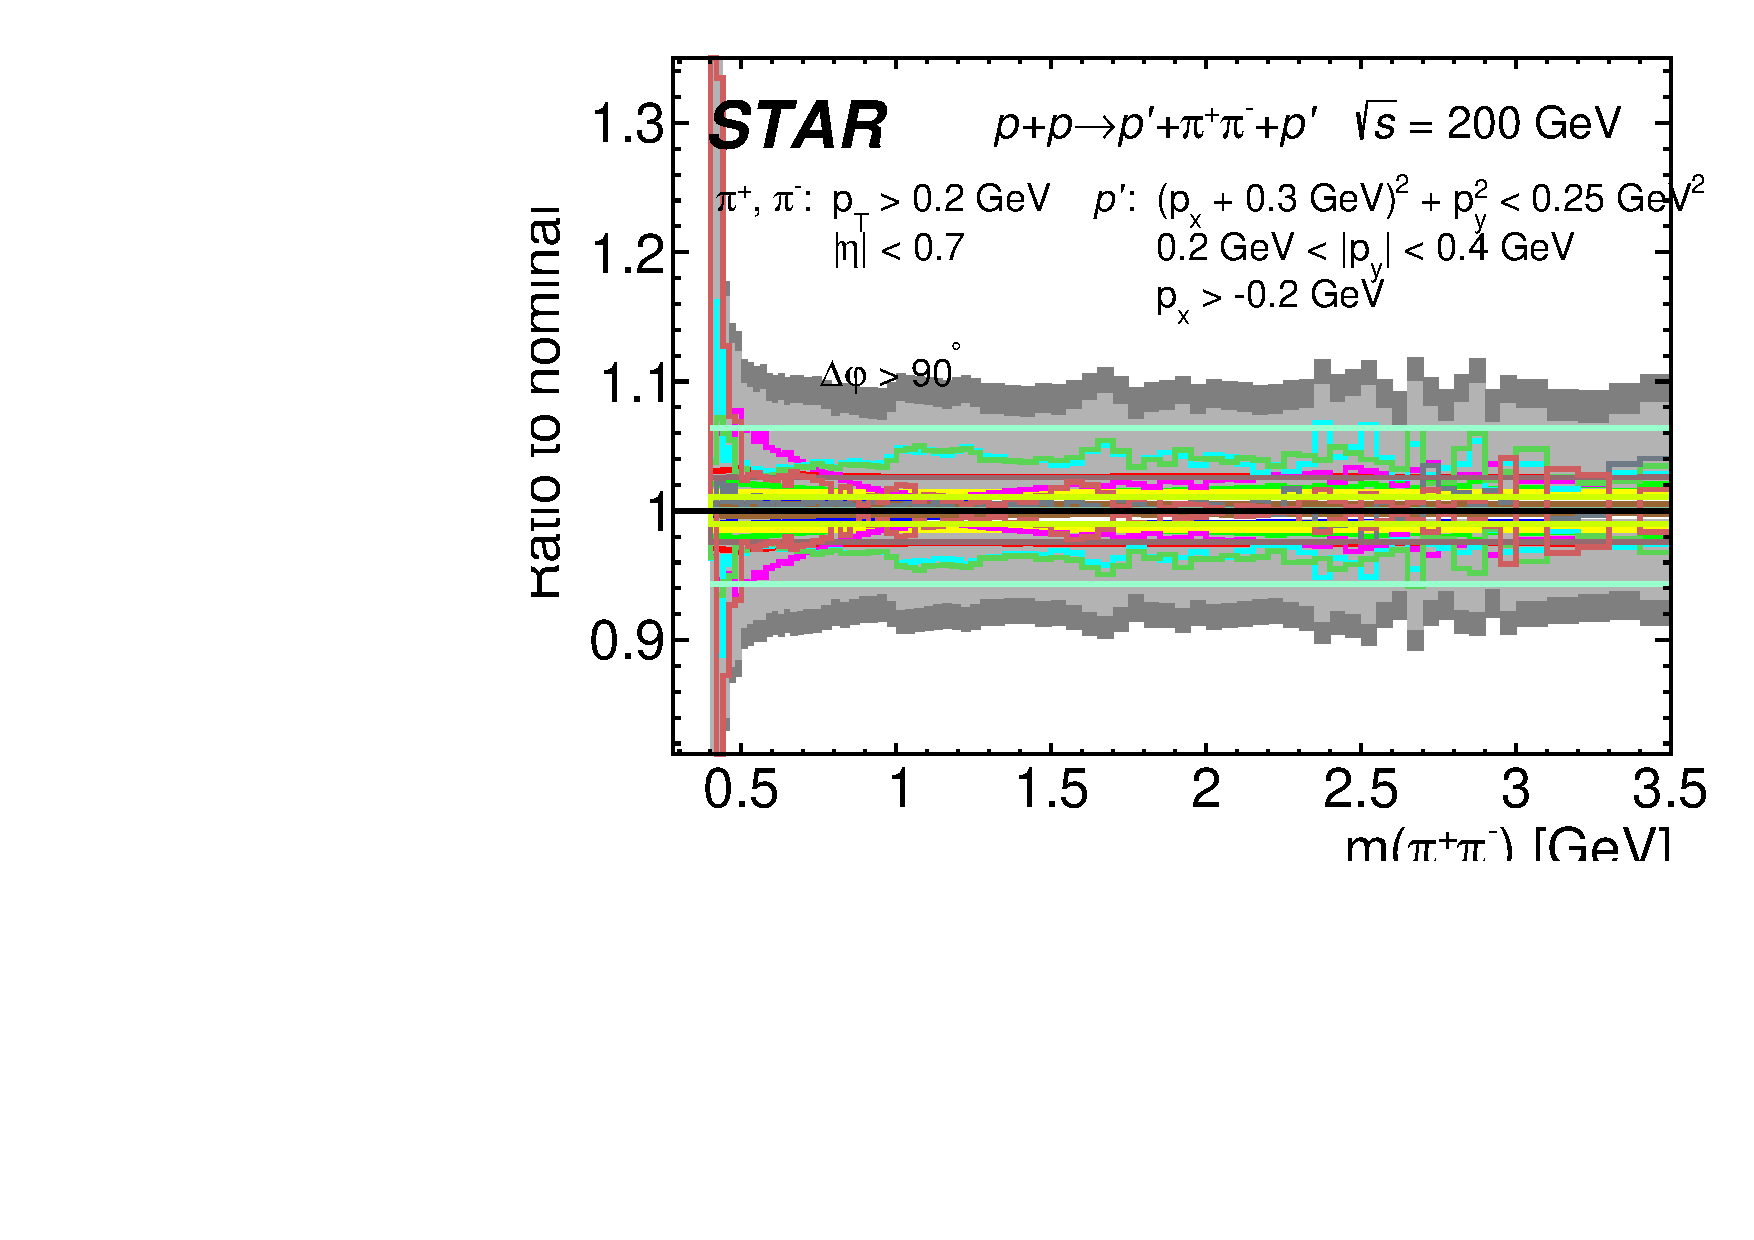
\includegraphics[width=.46\textwidth,page=1]{graphics/systematics/FinalResult_InvMass_DeltaPhiBin2_pion_Systematics2.pdf}
\hspace*{5pt}
\newline
\hspace*{5pt}
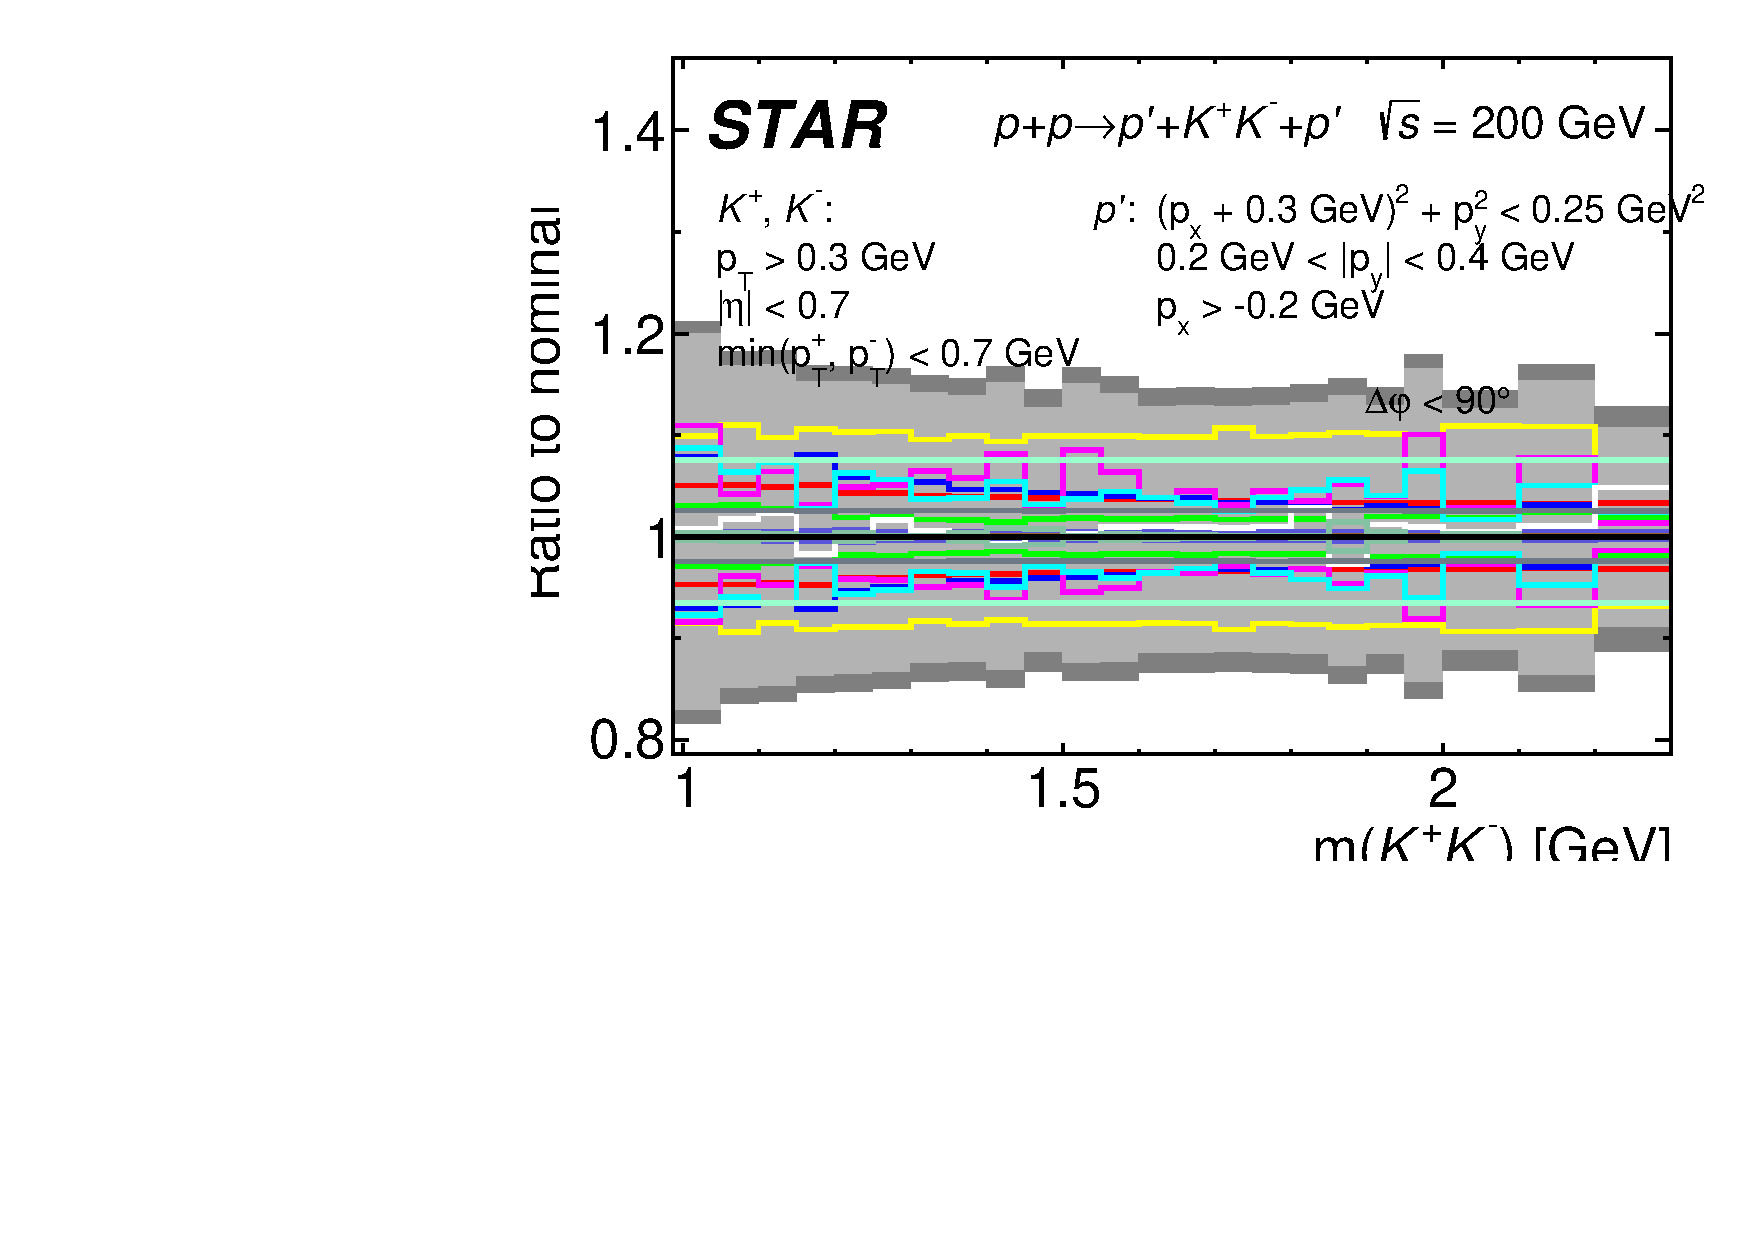
\includegraphics[width=.46\textwidth,page=1]{graphics/systematics/FinalResult_InvMass_DeltaPhiBin1_kaon_Systematics2.pdf}
\hfill
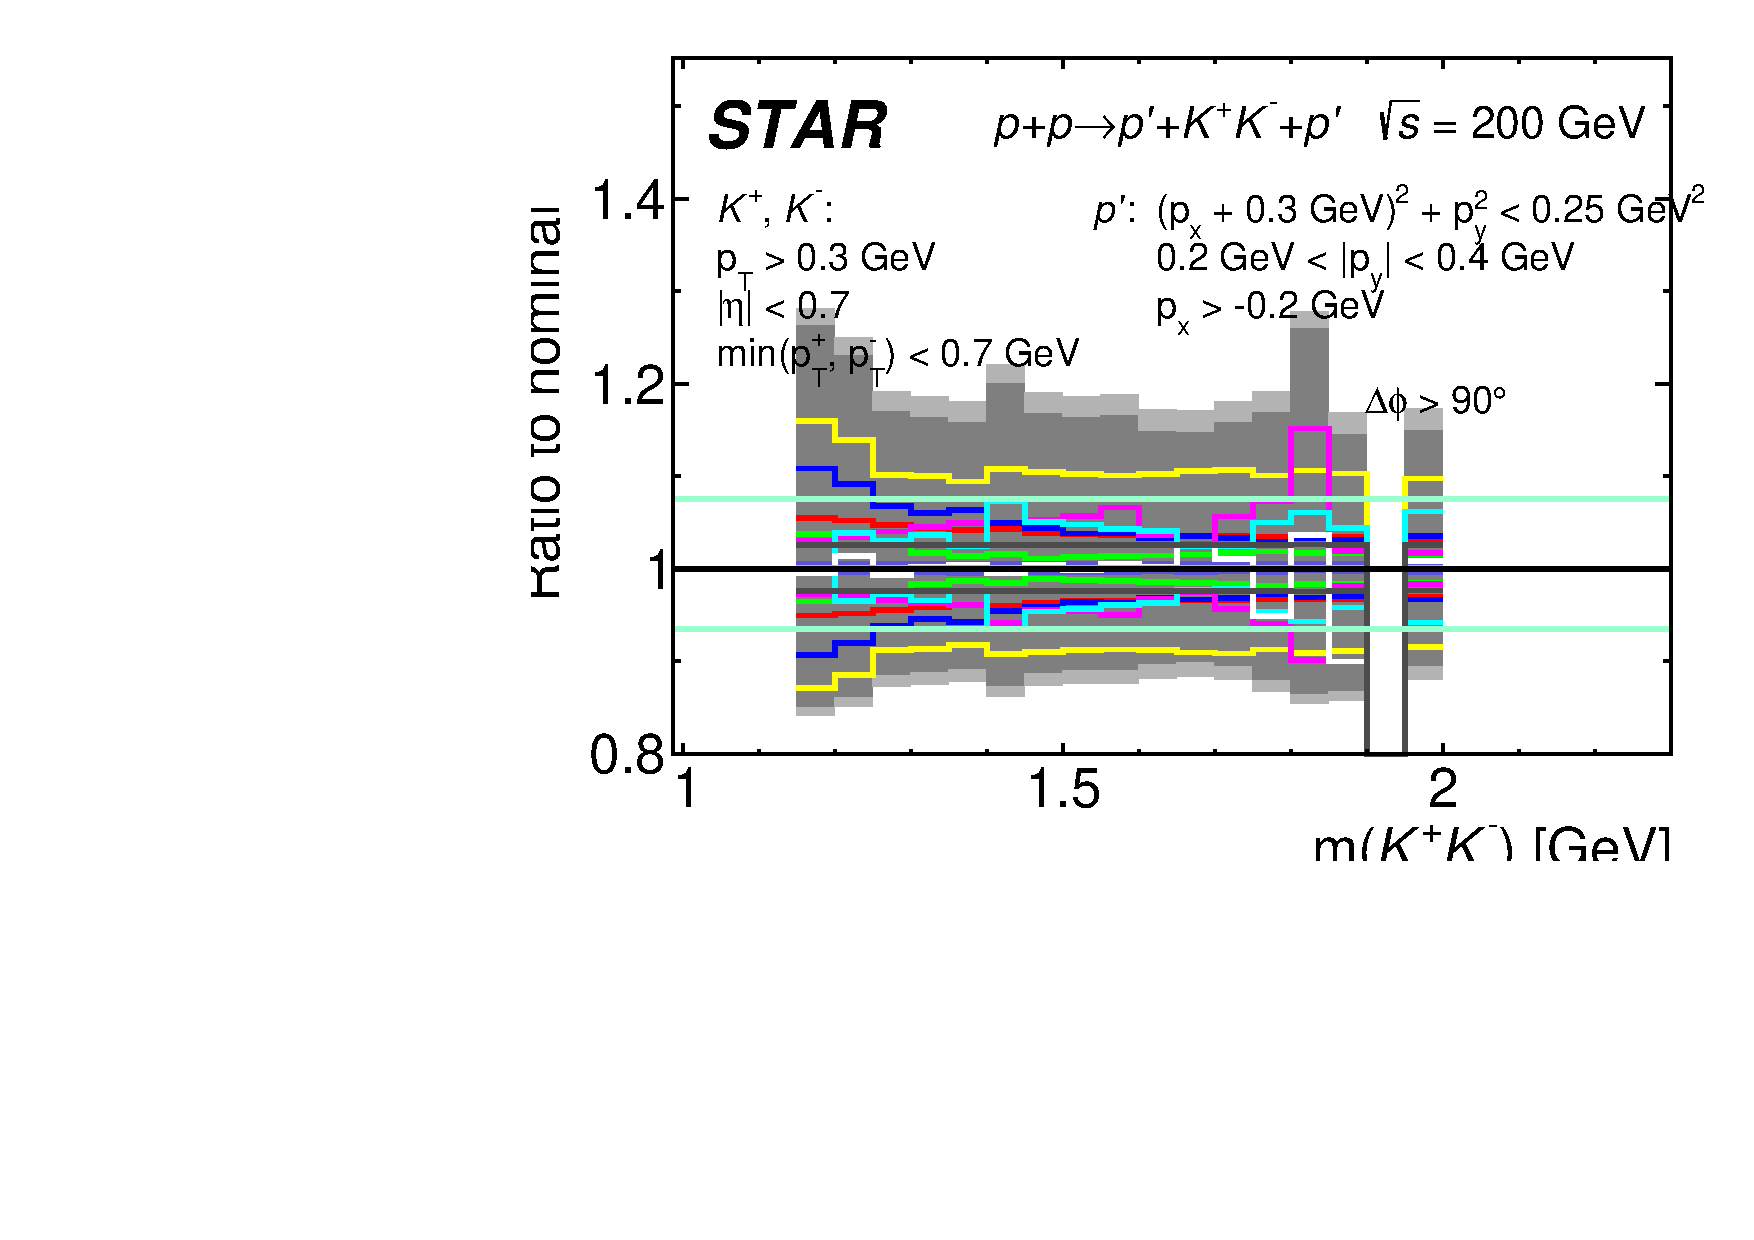
\includegraphics[width=.46\textwidth,page=1]{graphics/systematics/FinalResult_InvMass_DeltaPhiBin2_kaon_Systematics2.pdf}
\hspace*{5pt}
\newline
\hspace*{5pt}
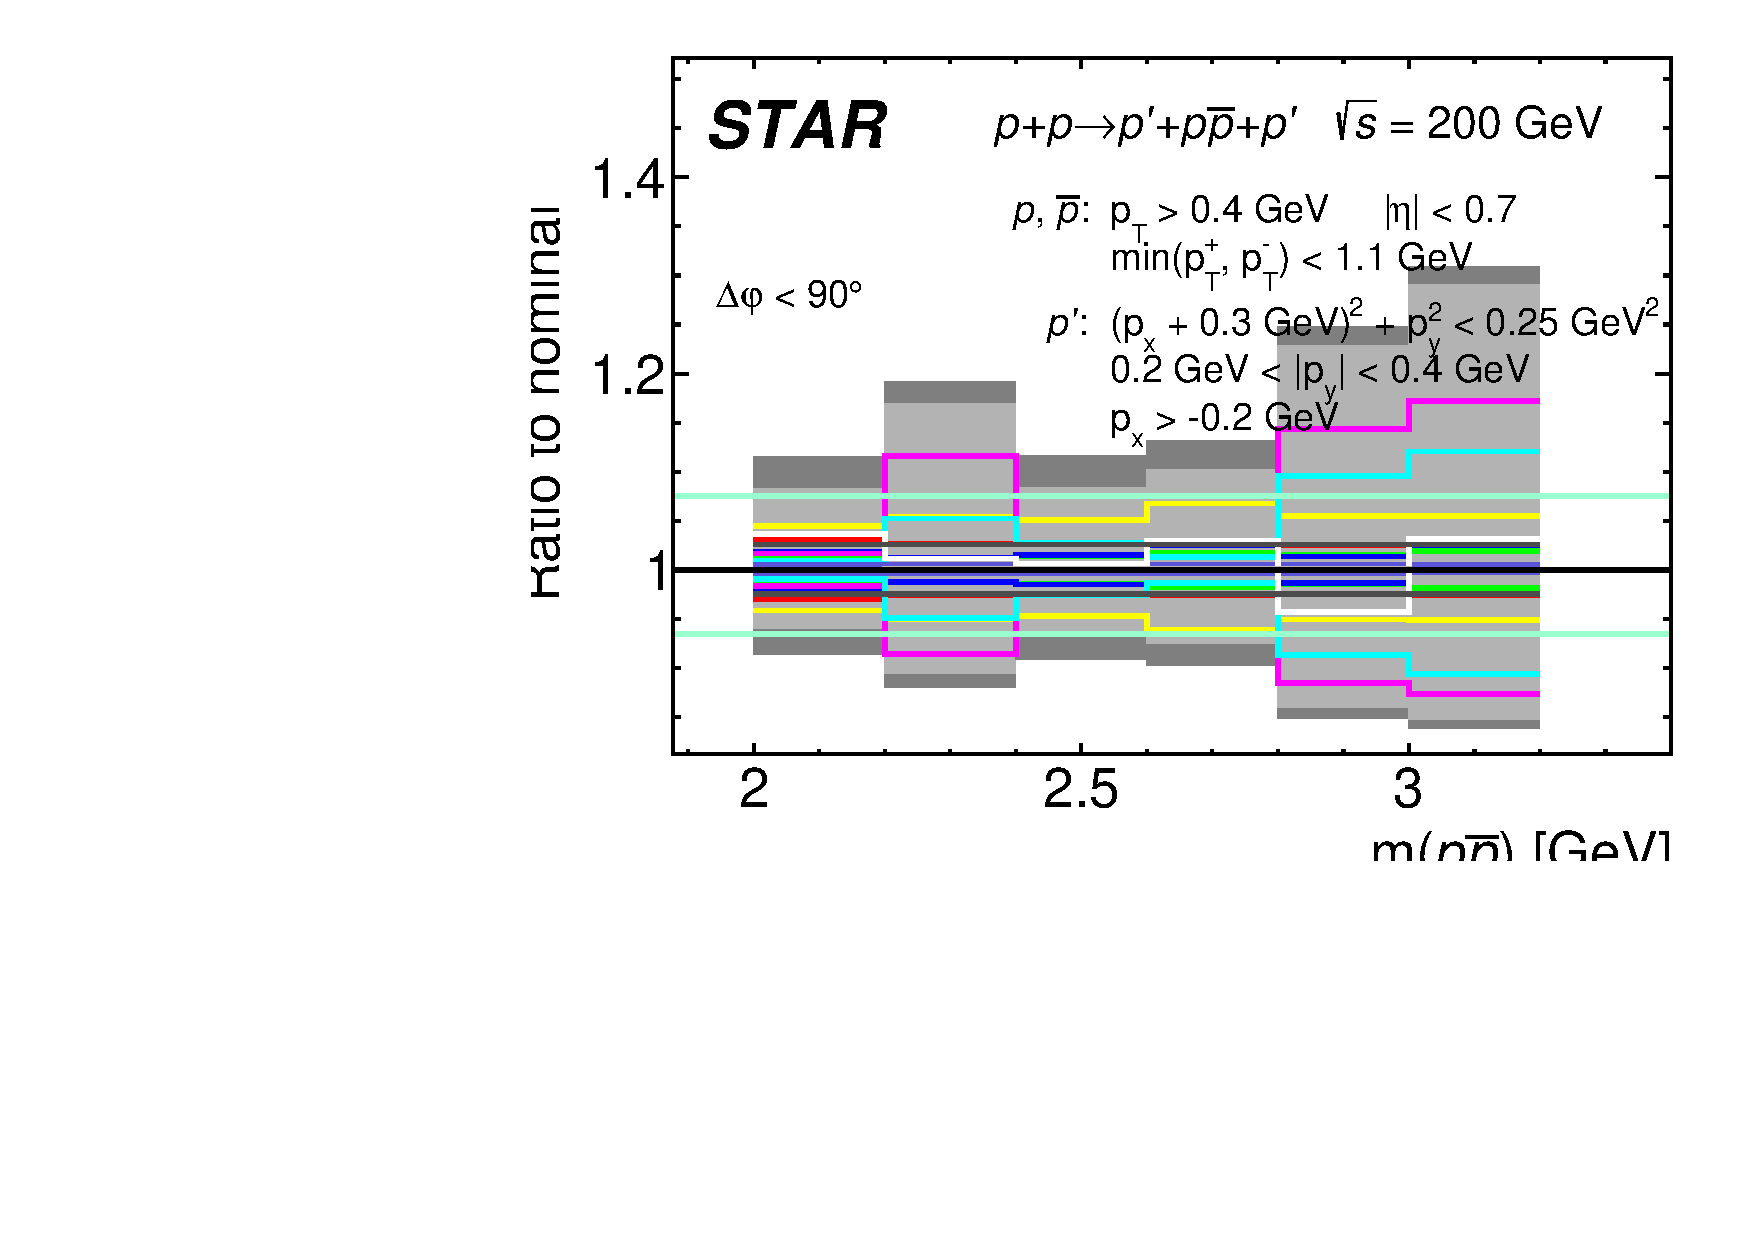
\includegraphics[width=.46\textwidth,page=1]{graphics/systematics/FinalResult_InvMass_DeltaPhiBin1_proton_Systematics2.pdf}
\hfill
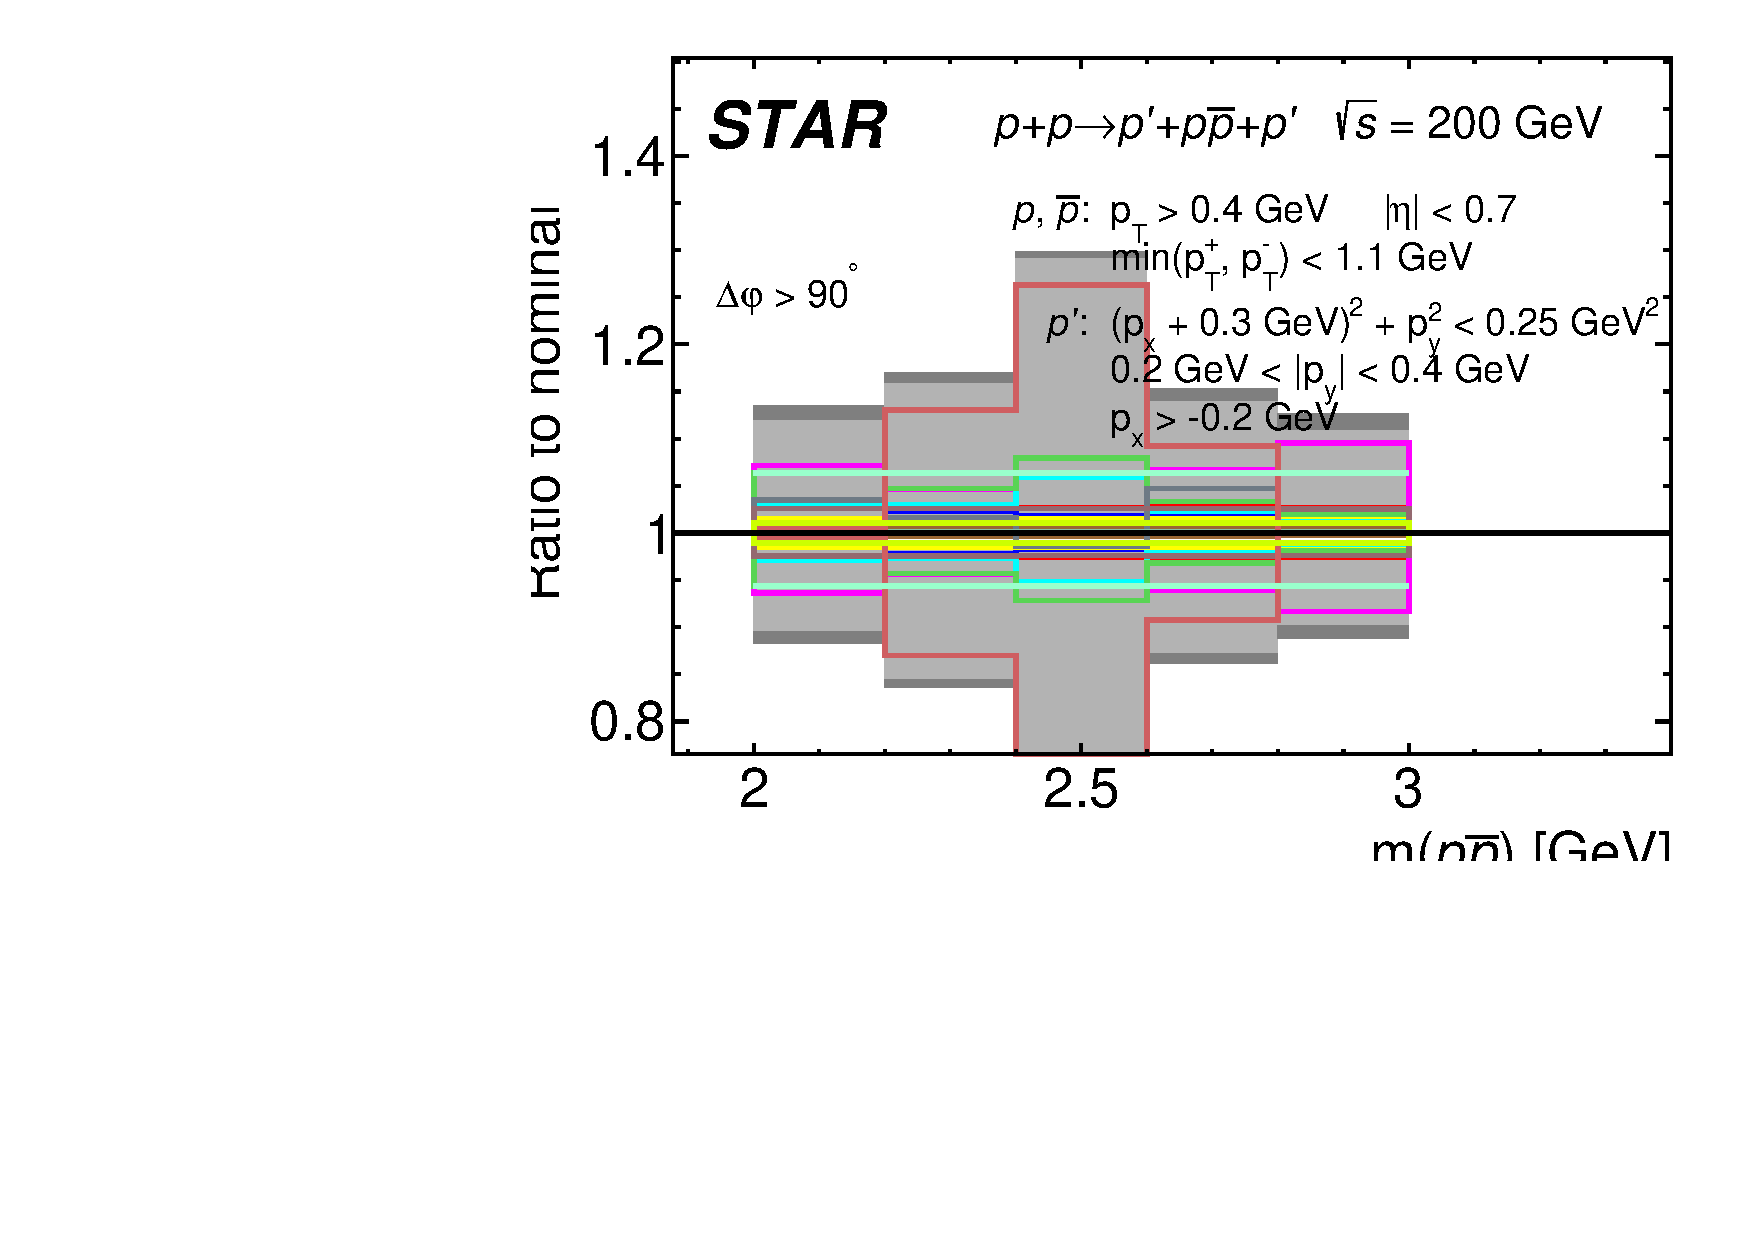
\includegraphics[width=.46\textwidth,page=1]{graphics/systematics/FinalResult_InvMass_DeltaPhiBin2_proton_Systematics2.pdf}
\hspace*{5pt}
%
\caption{Systematic uncertainties of the differential cross sections for CEP of charged particle pairs $\pi^+\pi^-$ (top), $K^+K^-$ (middle) and $p\bar{p}$ (bottom) as a function of the invariant mass of the pair in two $\Delta\phi$ regions: $\Delta\phi<90$ degree (left column) and $\Delta\phi>90$ degree (right column) measured in the fiducial region explained on the plots.}
\label{systematics_3}
\end{figure}
% %
% \FloatBarrier
% %
% Such correlation between resonances seen in mass spectrum and azimuthal angle between outgoing protons indicates factorization breaking between the two proton vertices. In the range $\Delta\phi<$ 90 degrees the DiMe model well describes both normalization and shape of mass spectrum at $m(\pi^+\pi^-)<$ 0.5 GeV.
% %
% In case of the cross section for CEP of $K^+K^-$ pairs the data do not show any significant asymmetry except possible widening
% of the peak at $f_2^\prime(1520)$ in the region $\Delta\phi<90$ degrees which may indicate an enhancement of additional resonances around 1.7~GeV in this configuration.
% %
% In case of the cross section for CEP of $p\bar{p}$ pairs data do not show any significant asymmetry except possible enhancement in the $2.2-2.4$ mass range for the $\Delta\phi>90$ degrees region.\\
% %
% \indent
% Due to high statistics of the two-pion sample it is possible to study the CEP of $\pi^+\pi^-$ pairs in more detail.
% Figure~\ref{systematics_4} shows the differential cross sections for CEP of $\pi^+\pi^-$ pairs as a function of the pair rapidity (left column), $\Delta\phi$ (middle column) and $|t_1+t_2|$ (right column) in three characteristic ranges of the invariant mass of the pair: $m(\pi^+\pi^-)<1.0$ GeV (mainly non-resonant production), $1.0< m(\pi^+\pi^-) <1.5$ GeV ($f_2(1270)$ mass range) and $m(\pi^+\pi^-)>1.5$ GeV (higher invariant masses).\\
% %
% \noindent
% Figure~\ref{systematics_4} shows the differential cross sections for CEP of different particle species pairs as a function of the pair rapidity (left column), of the difference of forward protons azimuthal angles (middle column) and of the sum of squares of the four-momenta transfers at the proton vertices (right column), for the three invariant mass ranges. In the case of the cross section $d\sigma/dy$ all models agree in shape with data in all three mass ranges except for the GenEx and DiMe predictions in the highest mass range where predictions is narrower.
% 
% Strong suppression of the fiducial cross section close to $90^\circ$ is due to the STAR RP acceptance while asymmetry $0^\circ$ vs. $180^\circ$ in the lowest mass region is due to the STAR TPC acceptance. $\Delta\phi$ distribution is sensitive to absorption  which are treated fully differentialy in DiMe generator and only on average in GenEx. This is consistent with generally better agreement between data and DiMe expectations except $f_2(1270)$ mass region. MBR model predicts symmetric $\Delta\phi$ distributions in all mass ranges which is not supported by the data.
% 
% The slope of the cross section as the function of $|t_1+t_2|$ is less steep in the $f_2(1270)$ mass region compared to other mass regions. In the low mass region the DiMe prediction has steeper slope compared to data.\\
%
\begin{figure}[h]
\centering
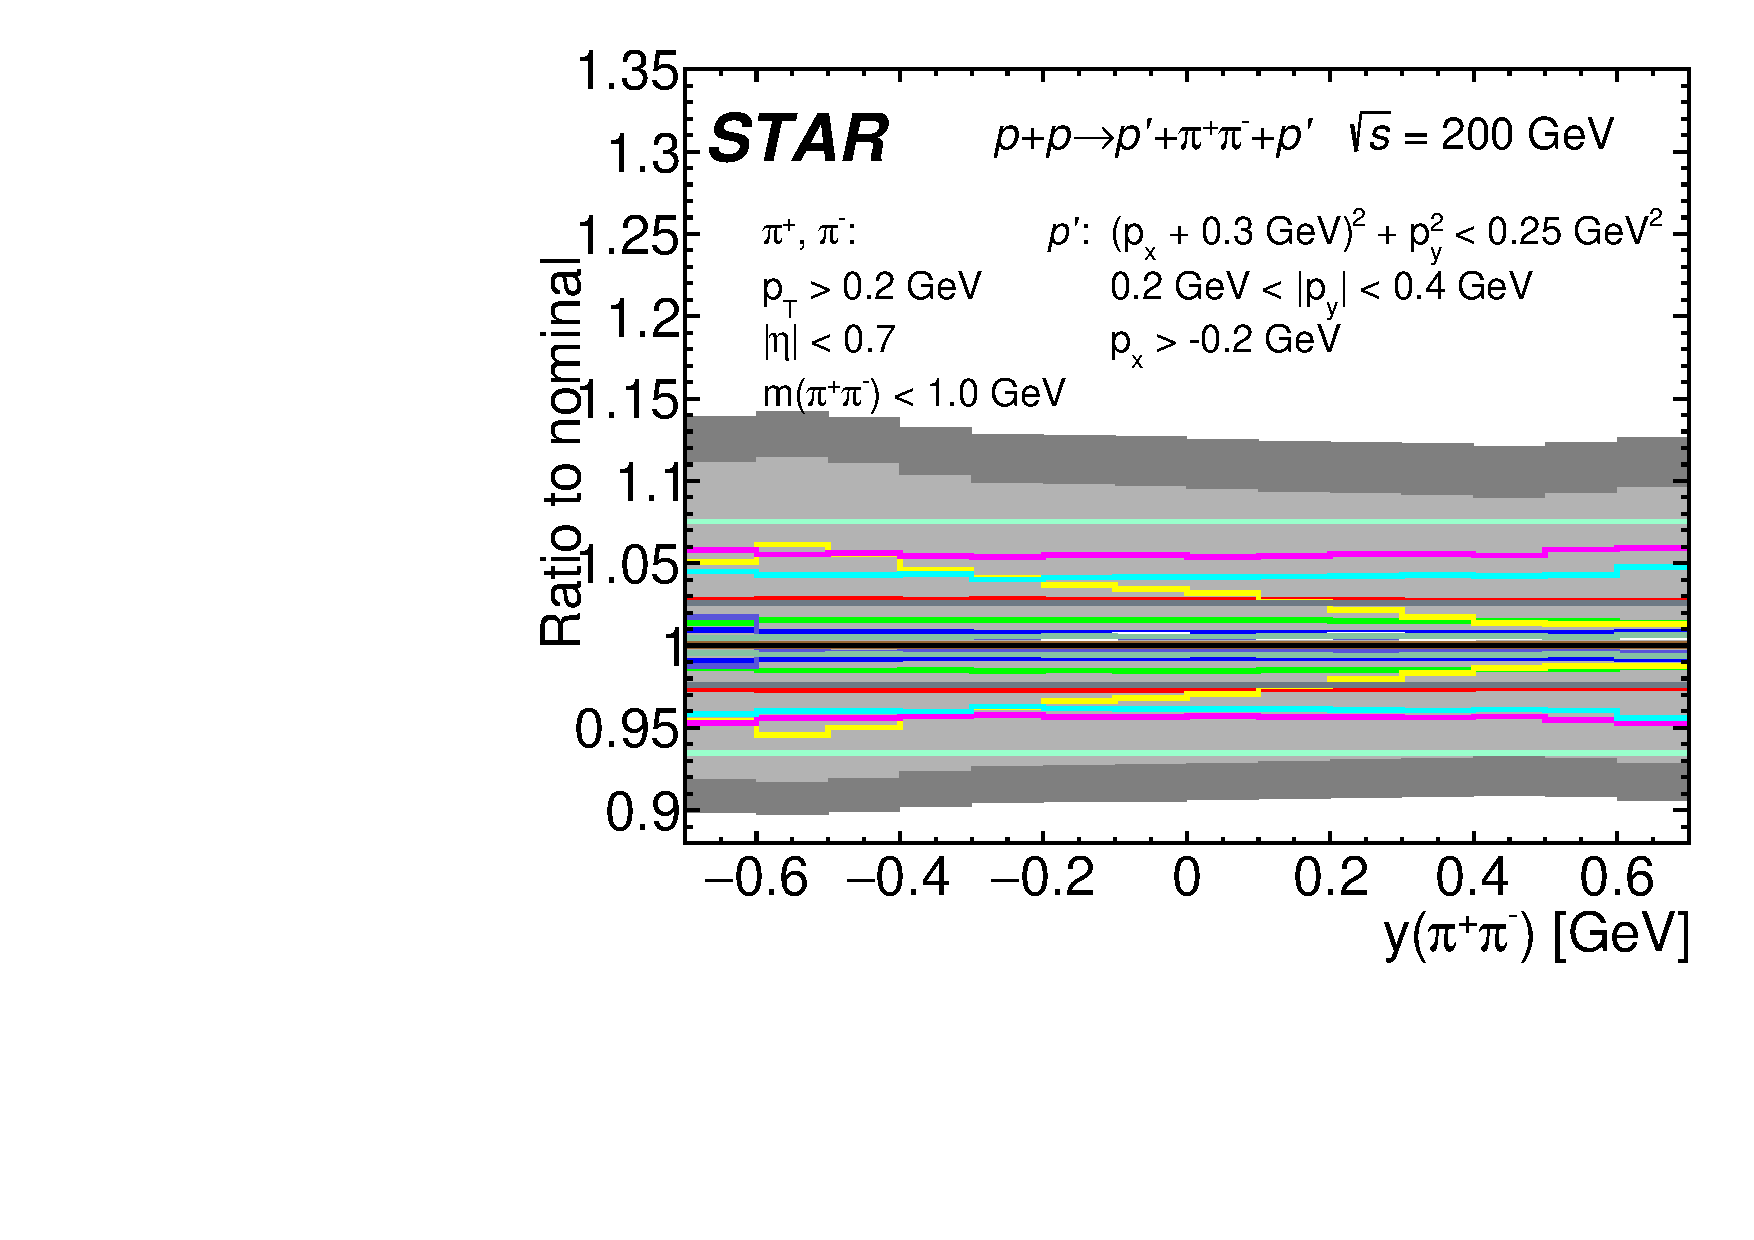
\includegraphics[width=.31\textwidth,page=1]{graphics/systematics/FinalResult_Rapidity_pion_MassBin_1_Systematics2.pdf}
\hfill
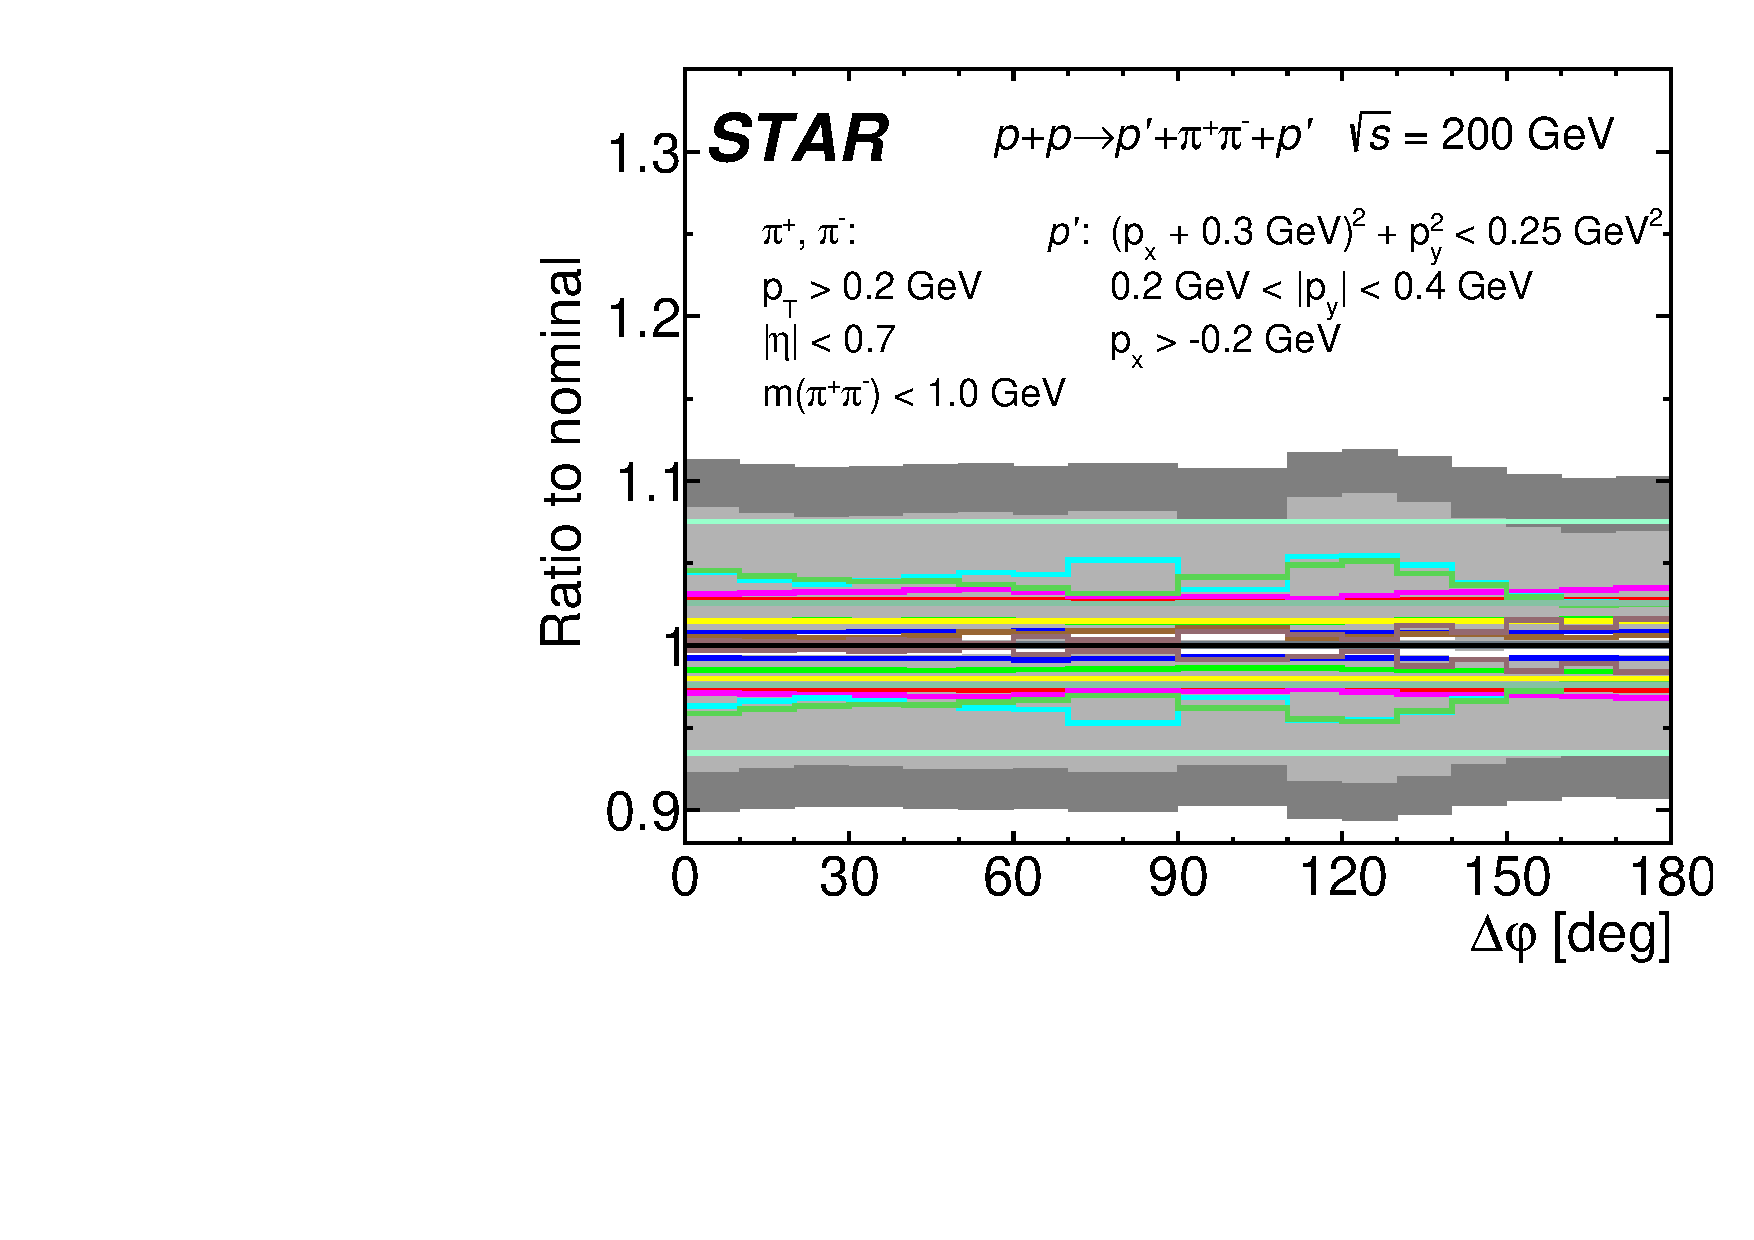
\includegraphics[width=.31\textwidth,page=1]{graphics/systematics/FinalResult_DeltaPhi_pion_MassBin_1_Systematics2.pdf}
\hfill
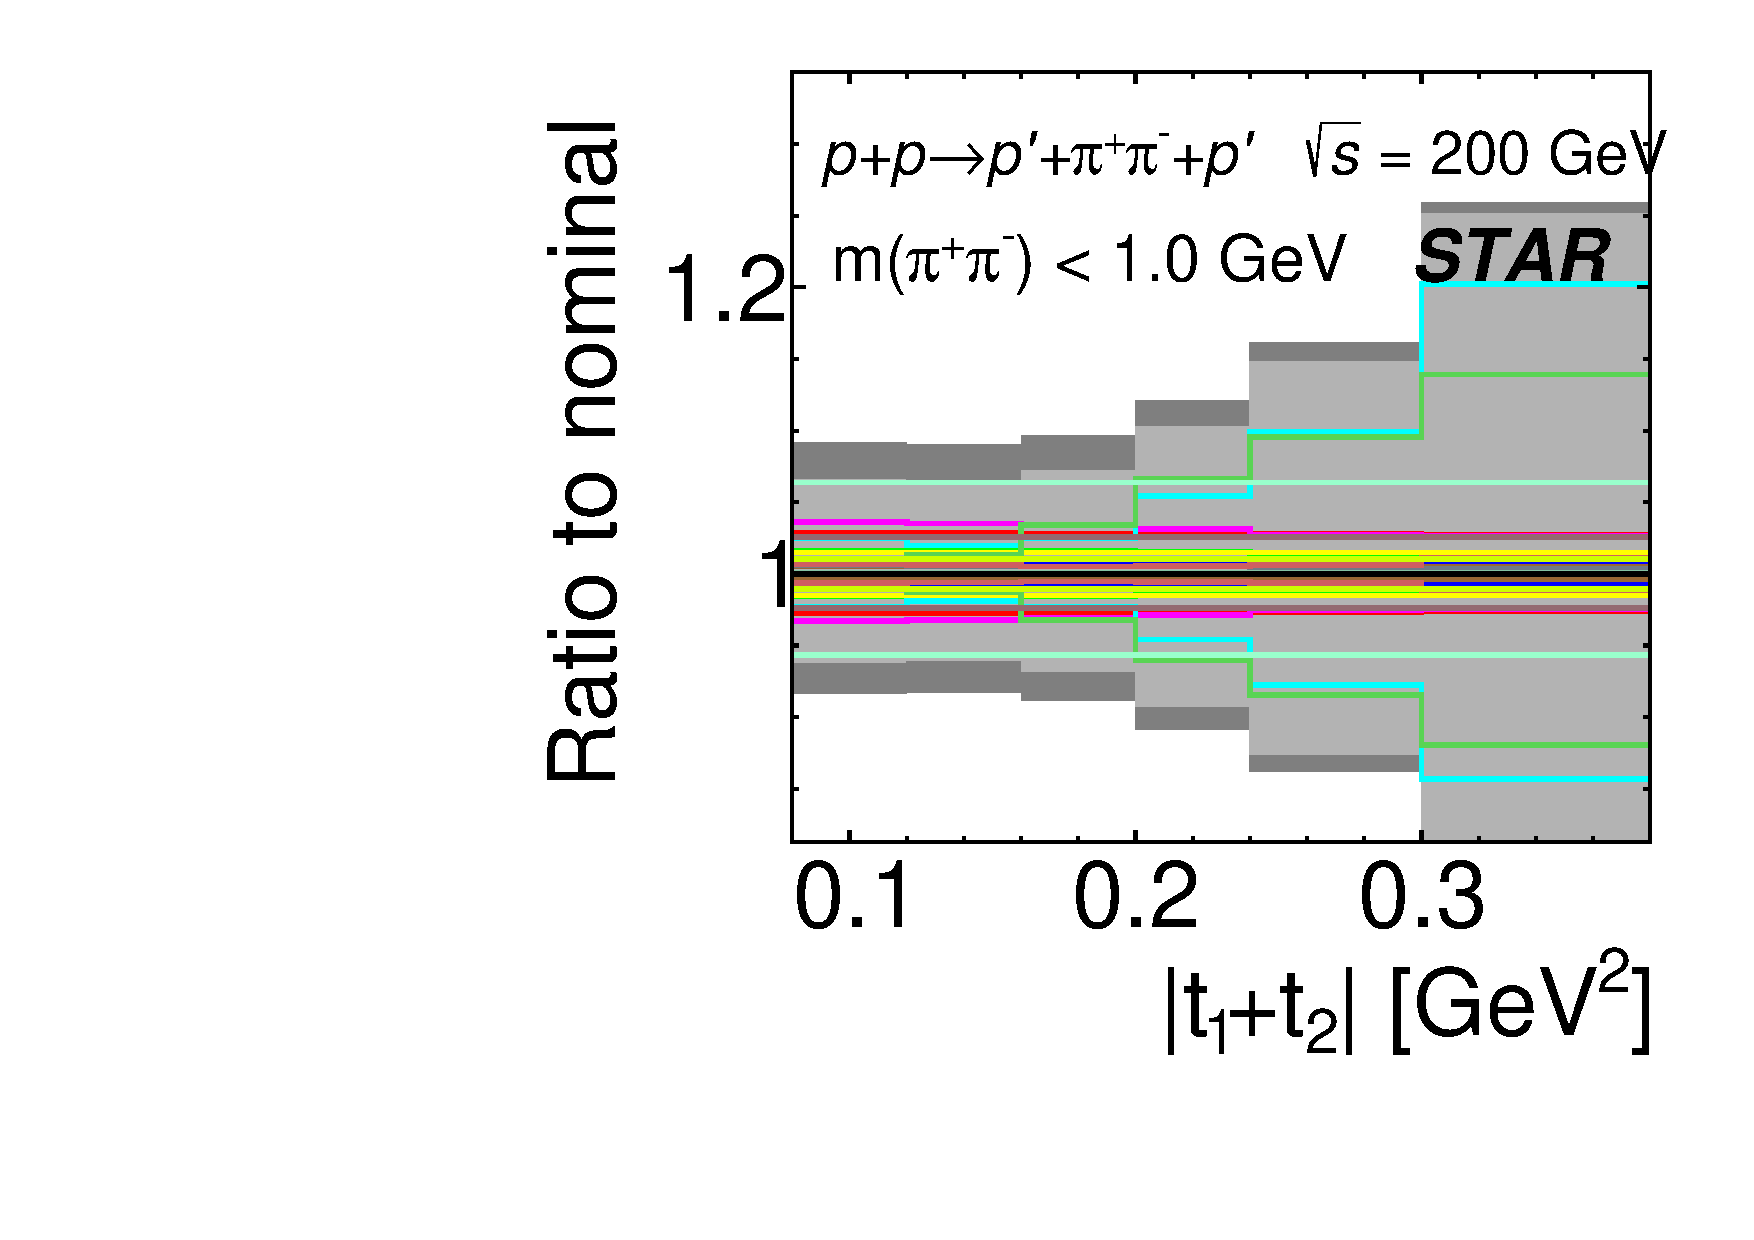
\includegraphics[width=.31\textwidth,page=1]{graphics/systematics/FinalResult_MandelstamTSum_pion_MassBin_1_Systematics2.pdf}
\newline
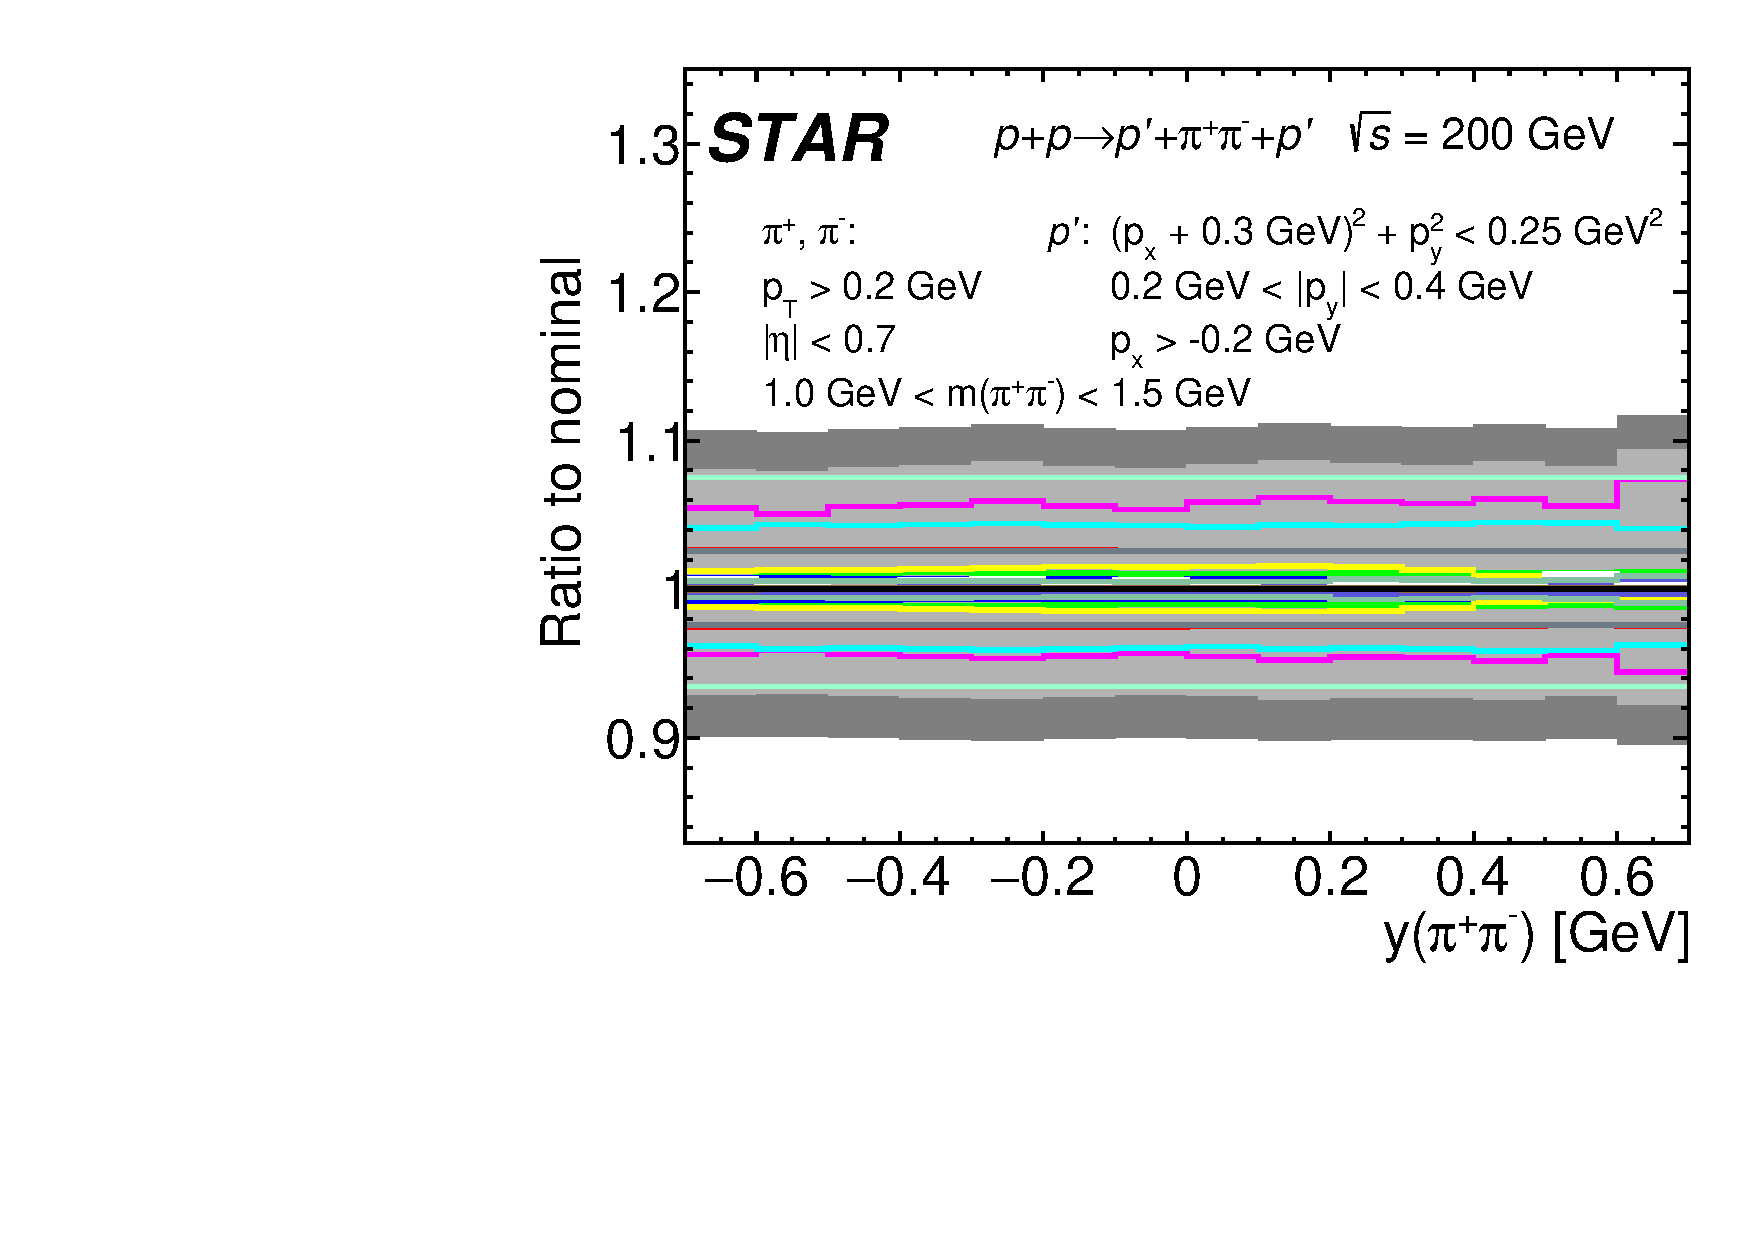
\includegraphics[width=.31\textwidth,page=1]{graphics/systematics/FinalResult_Rapidity_pion_MassBin_2_Systematics2.pdf}
\hfill
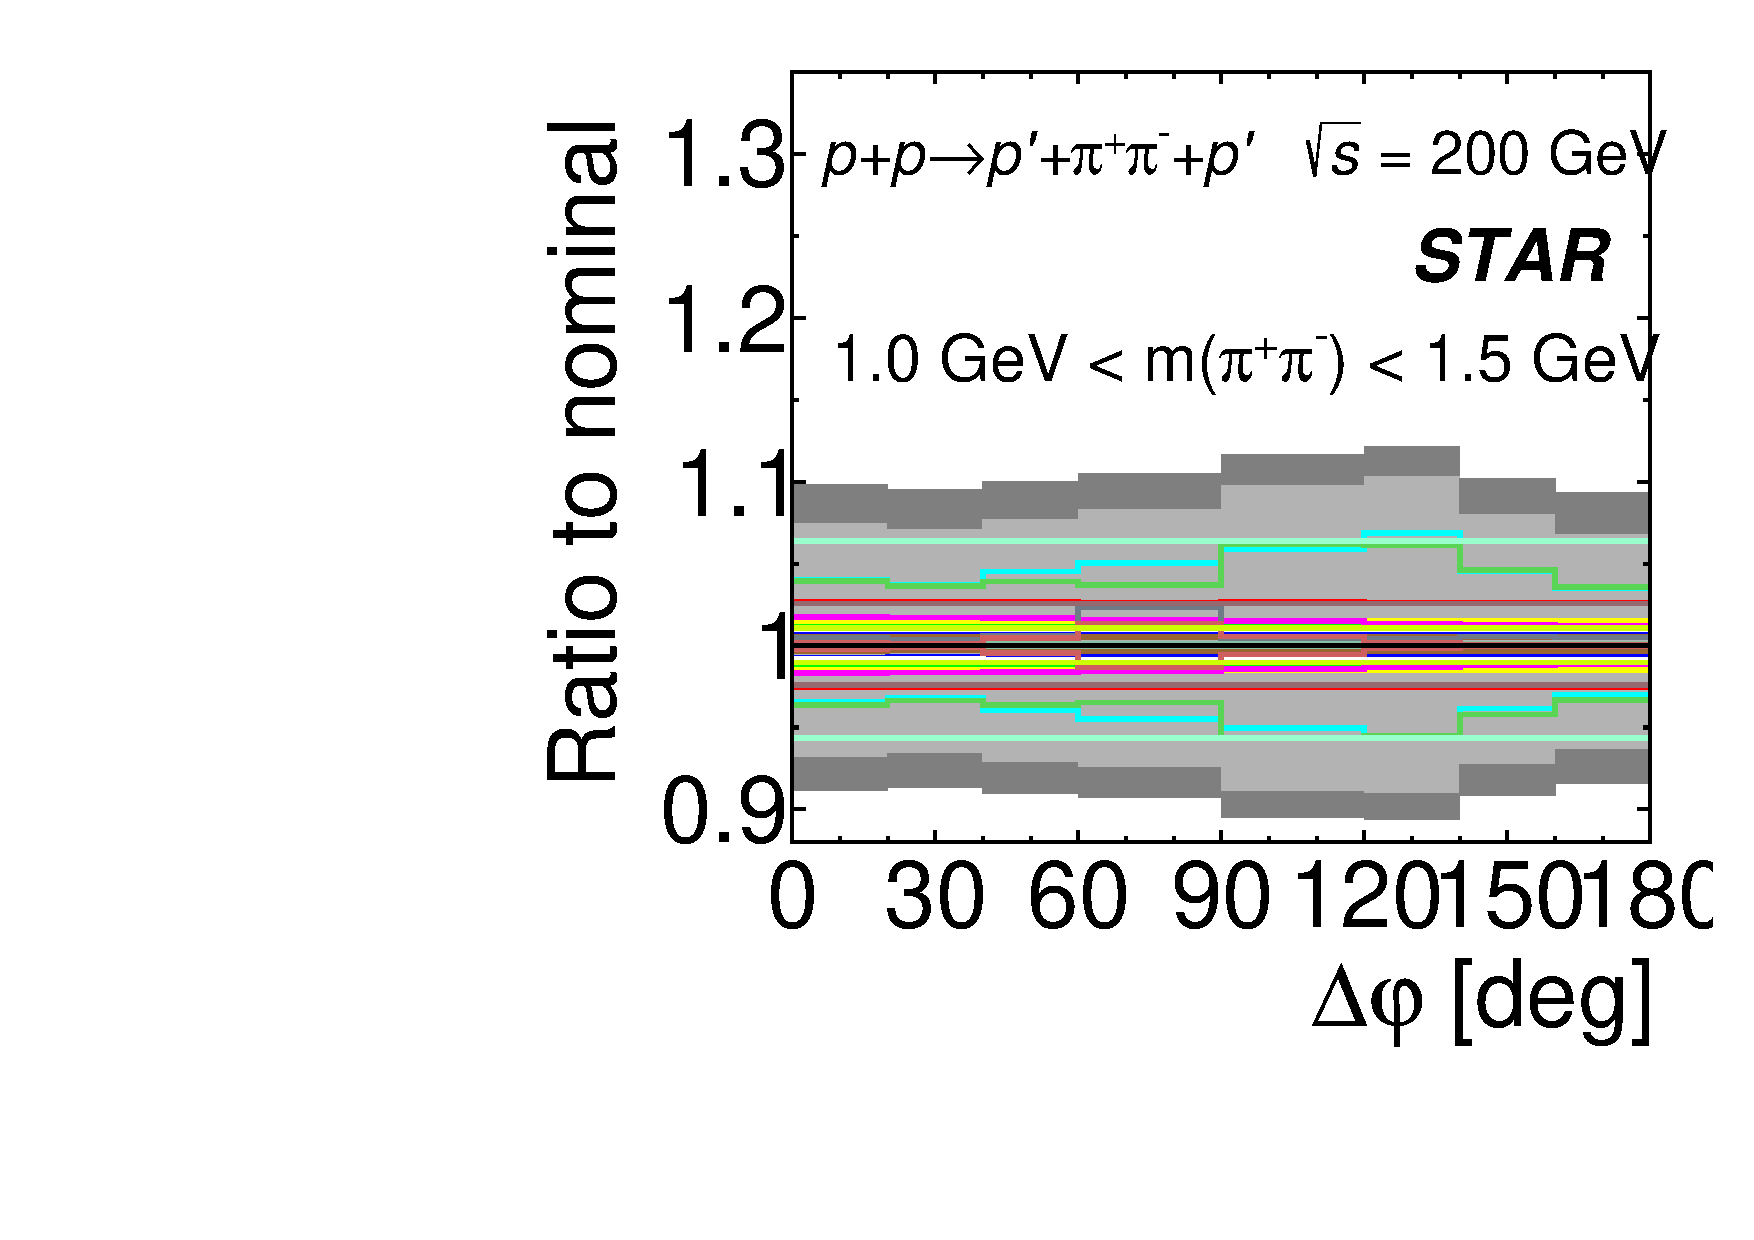
\includegraphics[width=.31\textwidth,page=1]{graphics/systematics/FinalResult_DeltaPhi_pion_MassBin_2_Systematics2.pdf}
\hfill
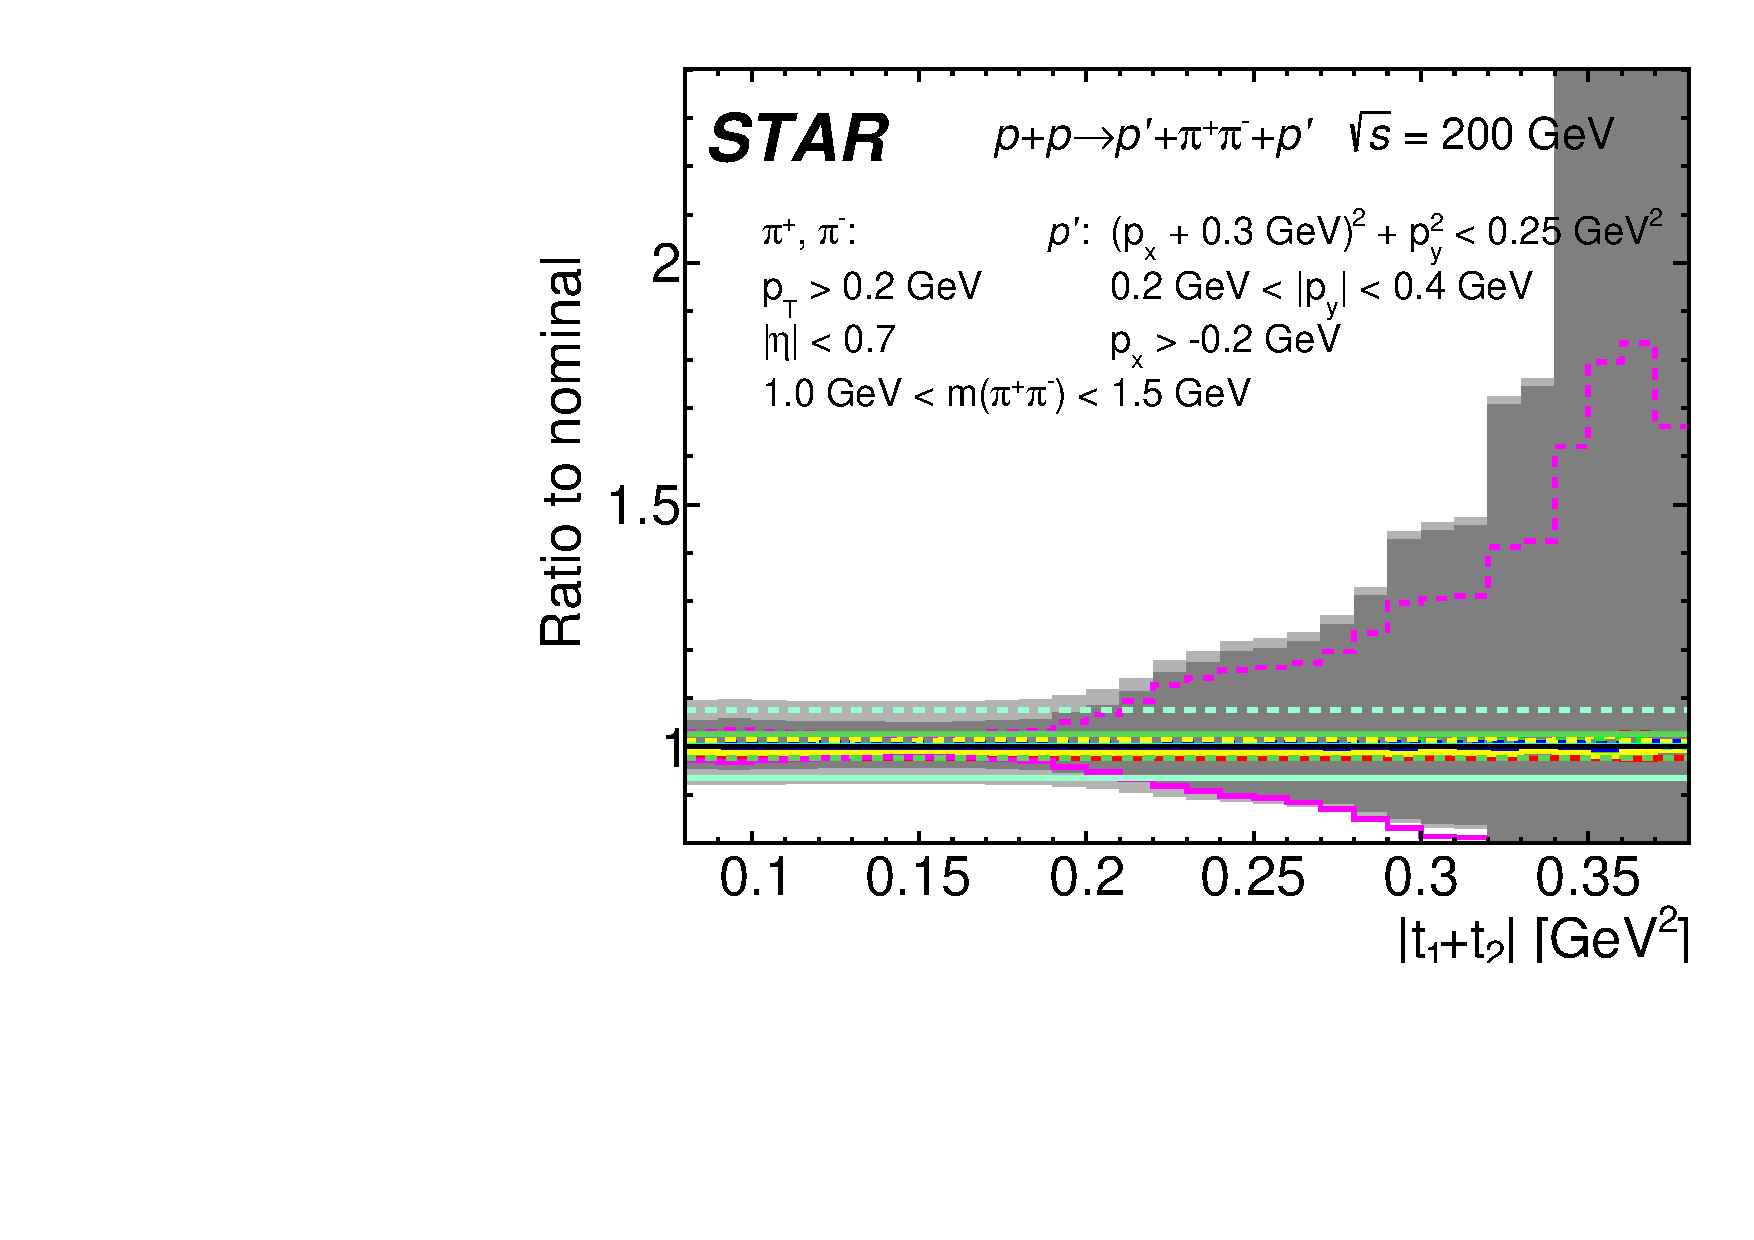
\includegraphics[width=.31\textwidth,page=1]{graphics/systematics/FinalResult_MandelstamTSum_pion_MassBin_2_Systematics2.pdf}
\newline
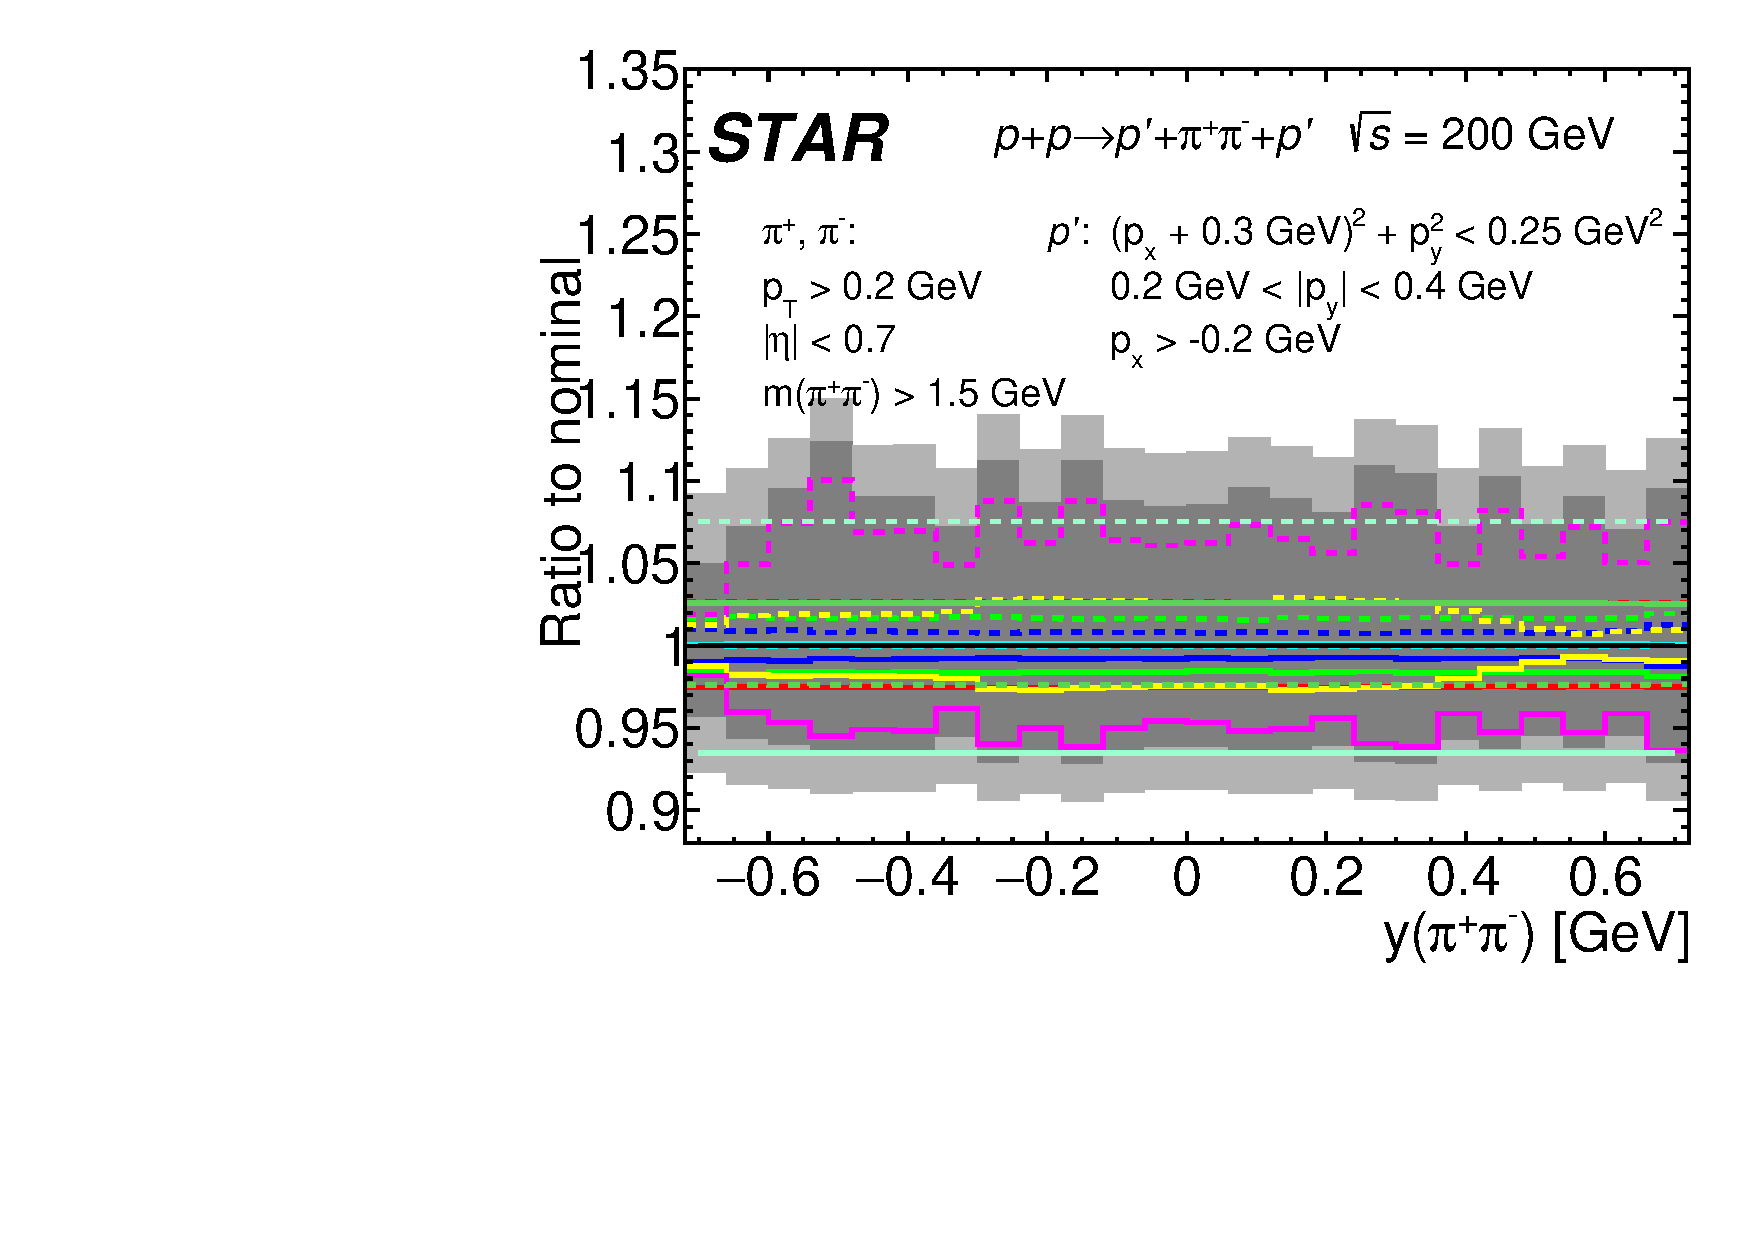
\includegraphics[width=.31\textwidth,page=1]{graphics/systematics/FinalResult_Rapidity_pion_MassBin_3_Systematics2.pdf}
\hfill
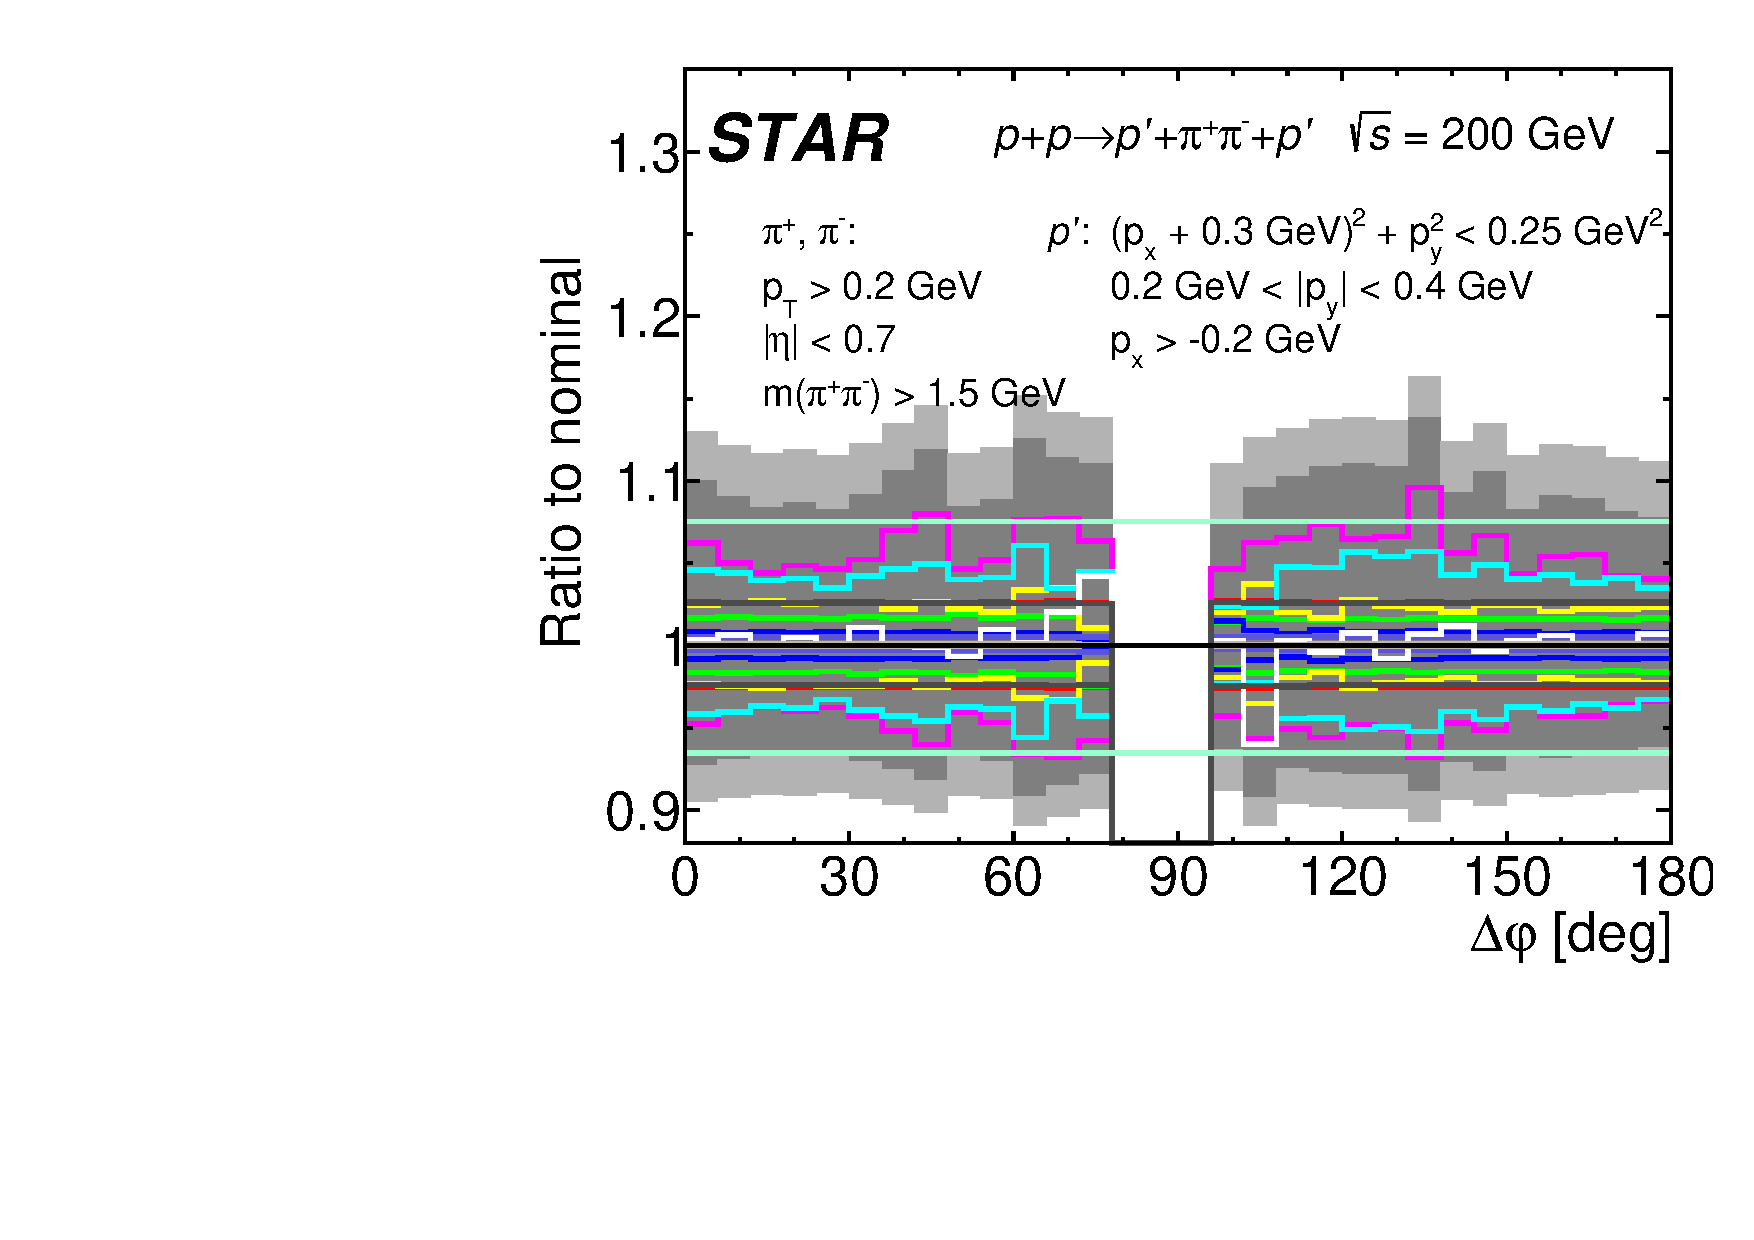
\includegraphics[width=.31\textwidth,page=1]{graphics/systematics/FinalResult_DeltaPhi_pion_MassBin_3_Systematics2.pdf}
\hfill
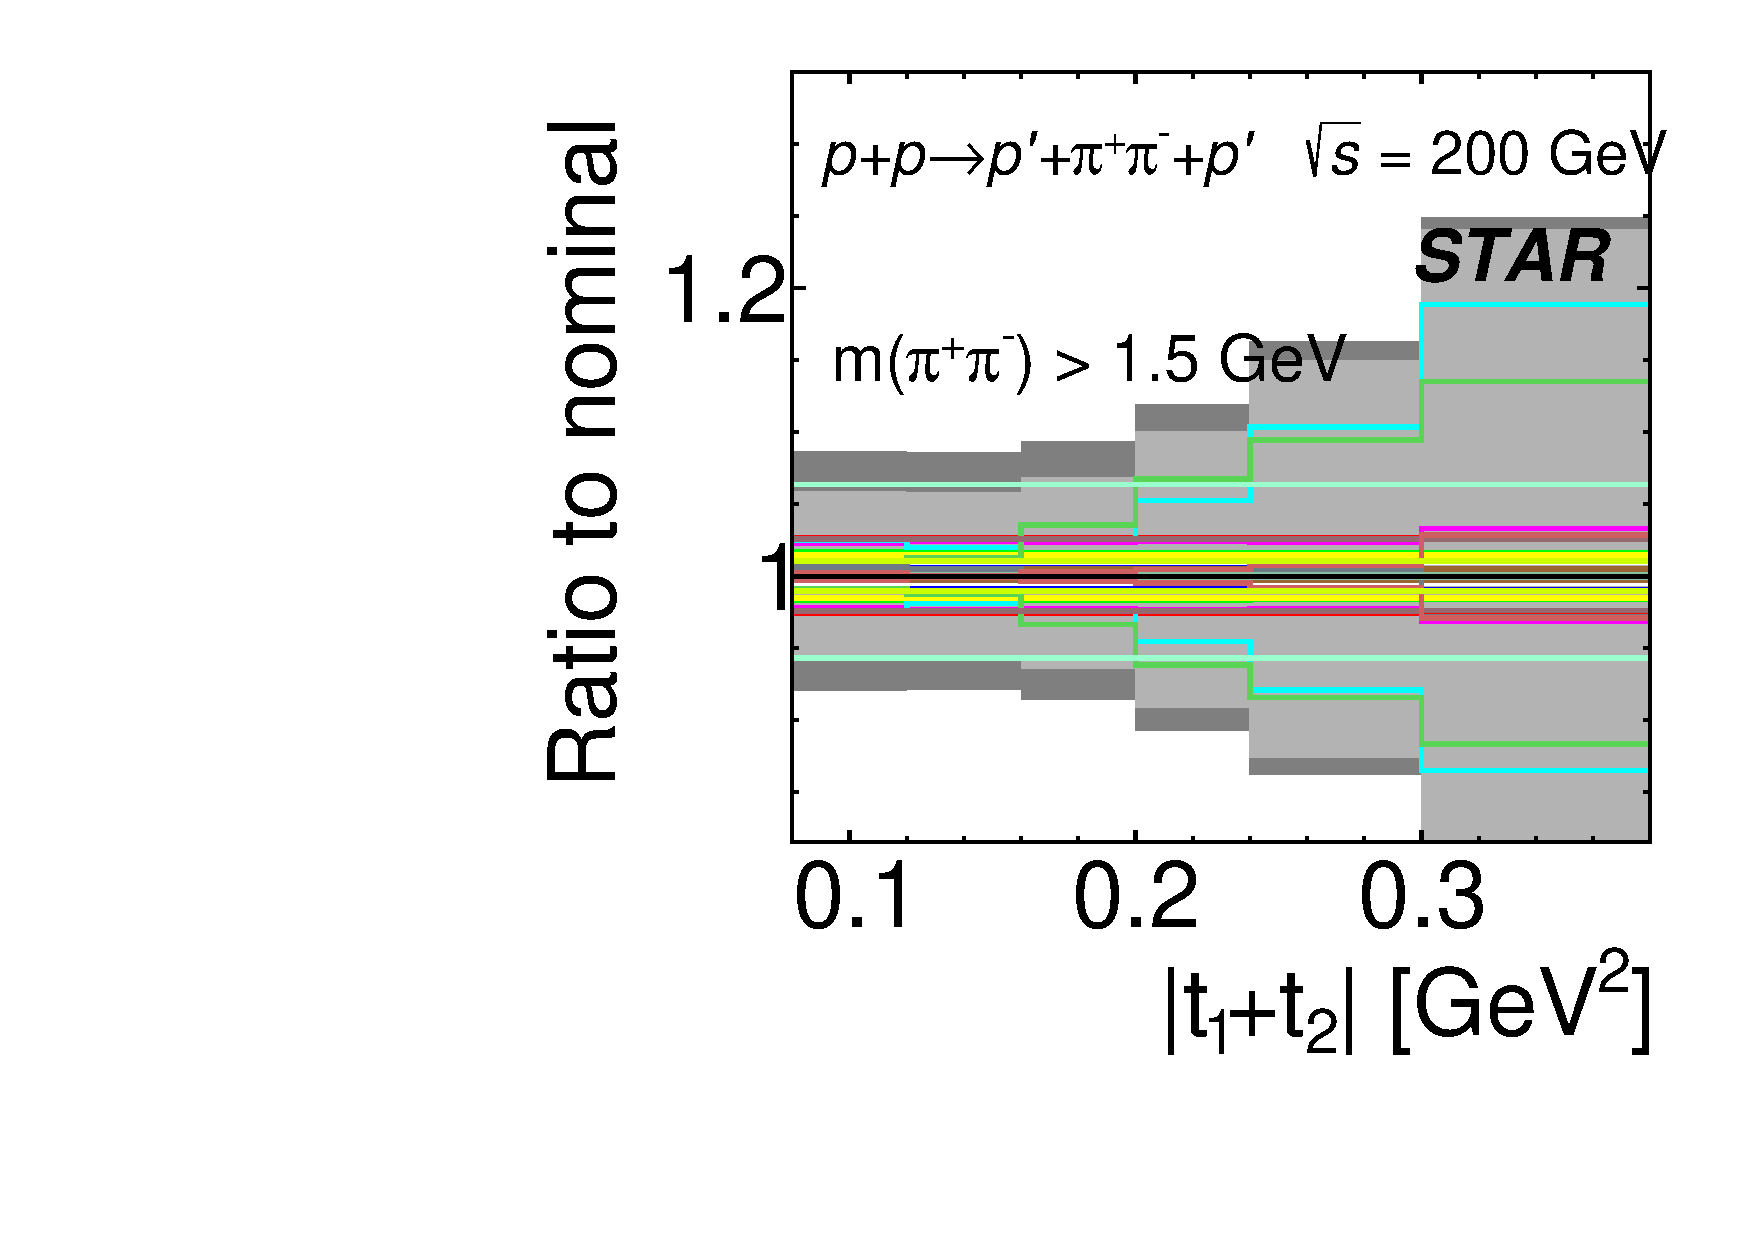
\includegraphics[width=.31\textwidth,page=1]{graphics/systematics/FinalResult_MandelstamTSum_pion_MassBin_3_Systematics2.pdf}
%
\caption{Systematic uncertainties of the differential cross sections for CEP of $\pi^+\pi^-$ pairs as a function of the rapidity of the pair (left column) difference of azimuthal angles of the forward scattered protons (middle column) and of the sum of the squares of the four-momenta losses in the proton vertices (right column) measured in the fiducial region explained on the plots, separately for three ranges of the $\pi^+\pi^-$ pair invariant mass: $m<1$ GeV (top), $1<m<1.5$ GeV (middle) and $m>1.5$ GeV (bottom).}
\label{systematics_4}
\end{figure}
%
%\FloatBarrier
%
\begin{figure}[h]
\centering
\hspace*{5pt}
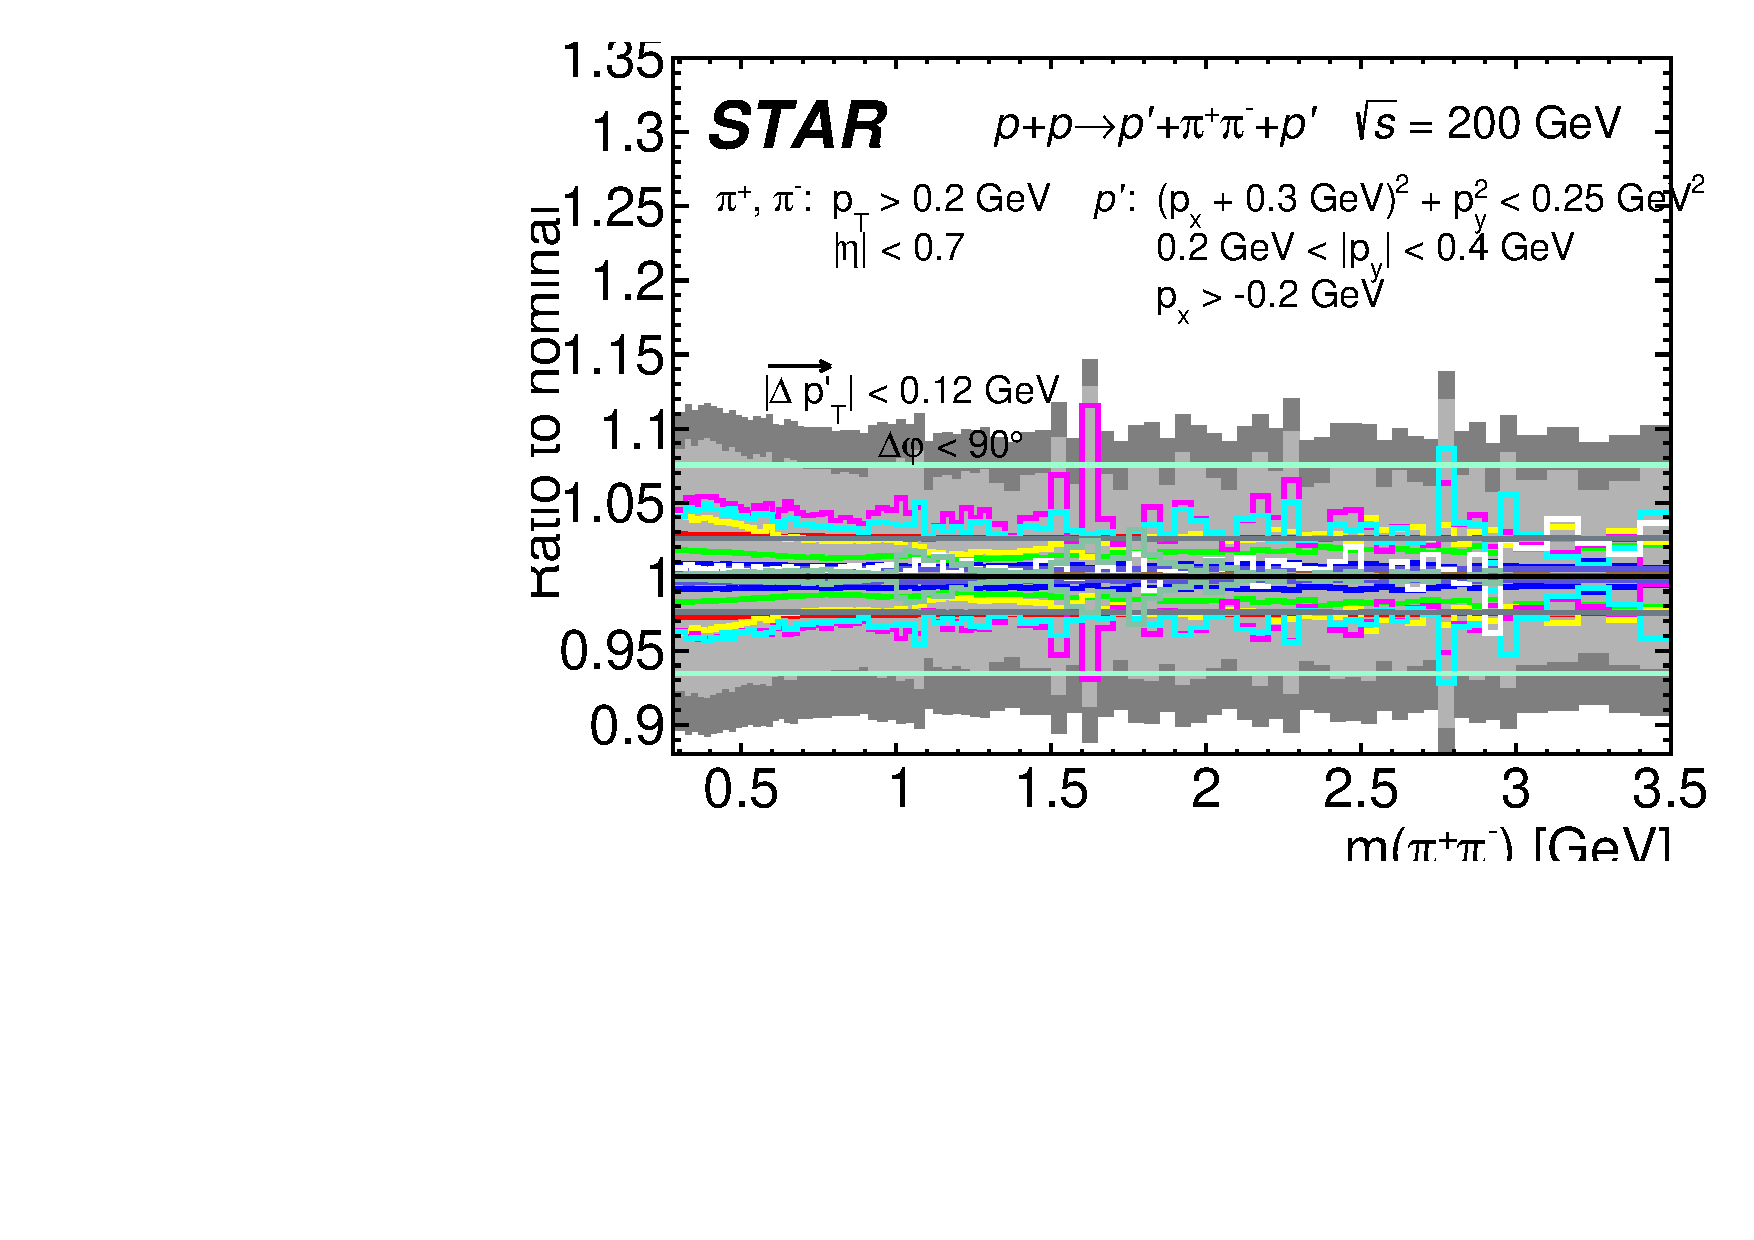
\includegraphics[width=.46\textwidth,page=1]{graphics/systematics/FinalResult_InvMass_pion_SmallDpt_DeltaPhiLessThan90_Systematics2.pdf}
\hfill
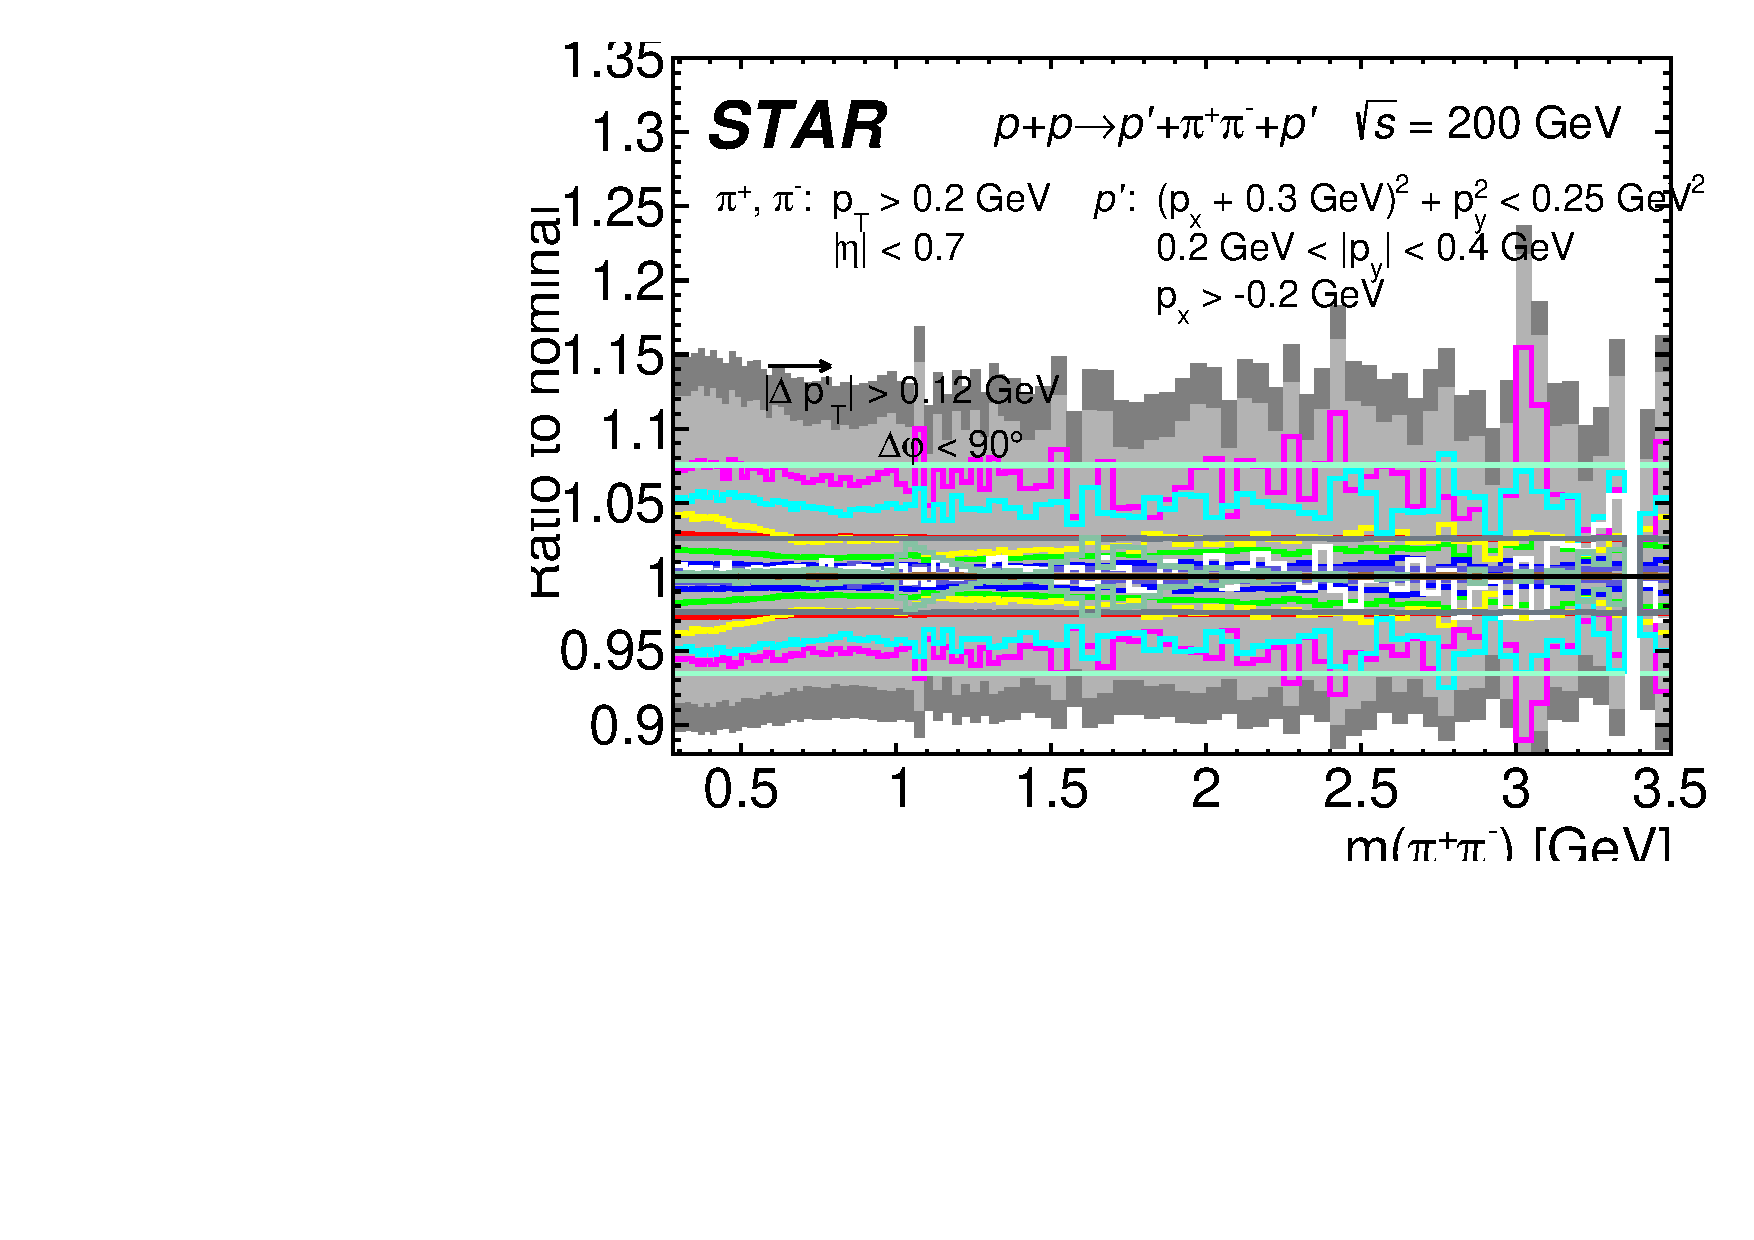
\includegraphics[width=.46\textwidth,page=1]{graphics/systematics/FinalResult_InvMass_pion_LargeDpt_DeltaPhiLessThan90_Systematics2.pdf}
\hspace*{5pt}
%
\caption{Systematic uncertainties of the differential cross sections $d\sigma/dm(\pi^+\pi^-)$ for CEP of $\pi^+\pi^-$ pairs in two $|\vec{p}_{1,T}^{\,\prime}-\vec{p}_{2,T}^{\,\prime}|$ regions: $|\vec{p}_{1,T}^{\,\prime}-\vec{p}_{2,T}^{\,\prime}|<0.12$ GeV (left) and $|\vec{p}_{1,T}^{\,\prime}-\vec{p}_{2,T}^{\,\prime}|>0.12$ GeV (right)  in the fiducial region and $\Delta\phi<90$ degree.}
\label{systematics_5}
\end{figure}


% We have also studied angular distributions of the charged particles produced in the final state. This can be done in various reference frames. However, for an easy comparison with theoretical predictions we use here the Collins-Soper \cite{cs_frame} reference frame also used e.g. in Ref.~\cite{lebiedowicz_3}. Collins-Soper frame is the centre-of-mass frame of the charged particles pair with the $z$-axis making equal angles with the beam protons momenta which in addition define the new $x-z$ plane. It can be reached from the laboratory frame (proton-proton c.m.s.) in two steps. First, boost along the $z$-axis to an intermediate frame in which the pair longitudinal momentum is equal to zero. In this frame the beam protons momenta remain parallel to the $z$-axis and the transverse momentum of the pair remains unchanged. Second, boost in the direction of the transverse momentum of the pair, to get to the pair c.m.s. frame. 
%
\begin{figure}[h]
\centering
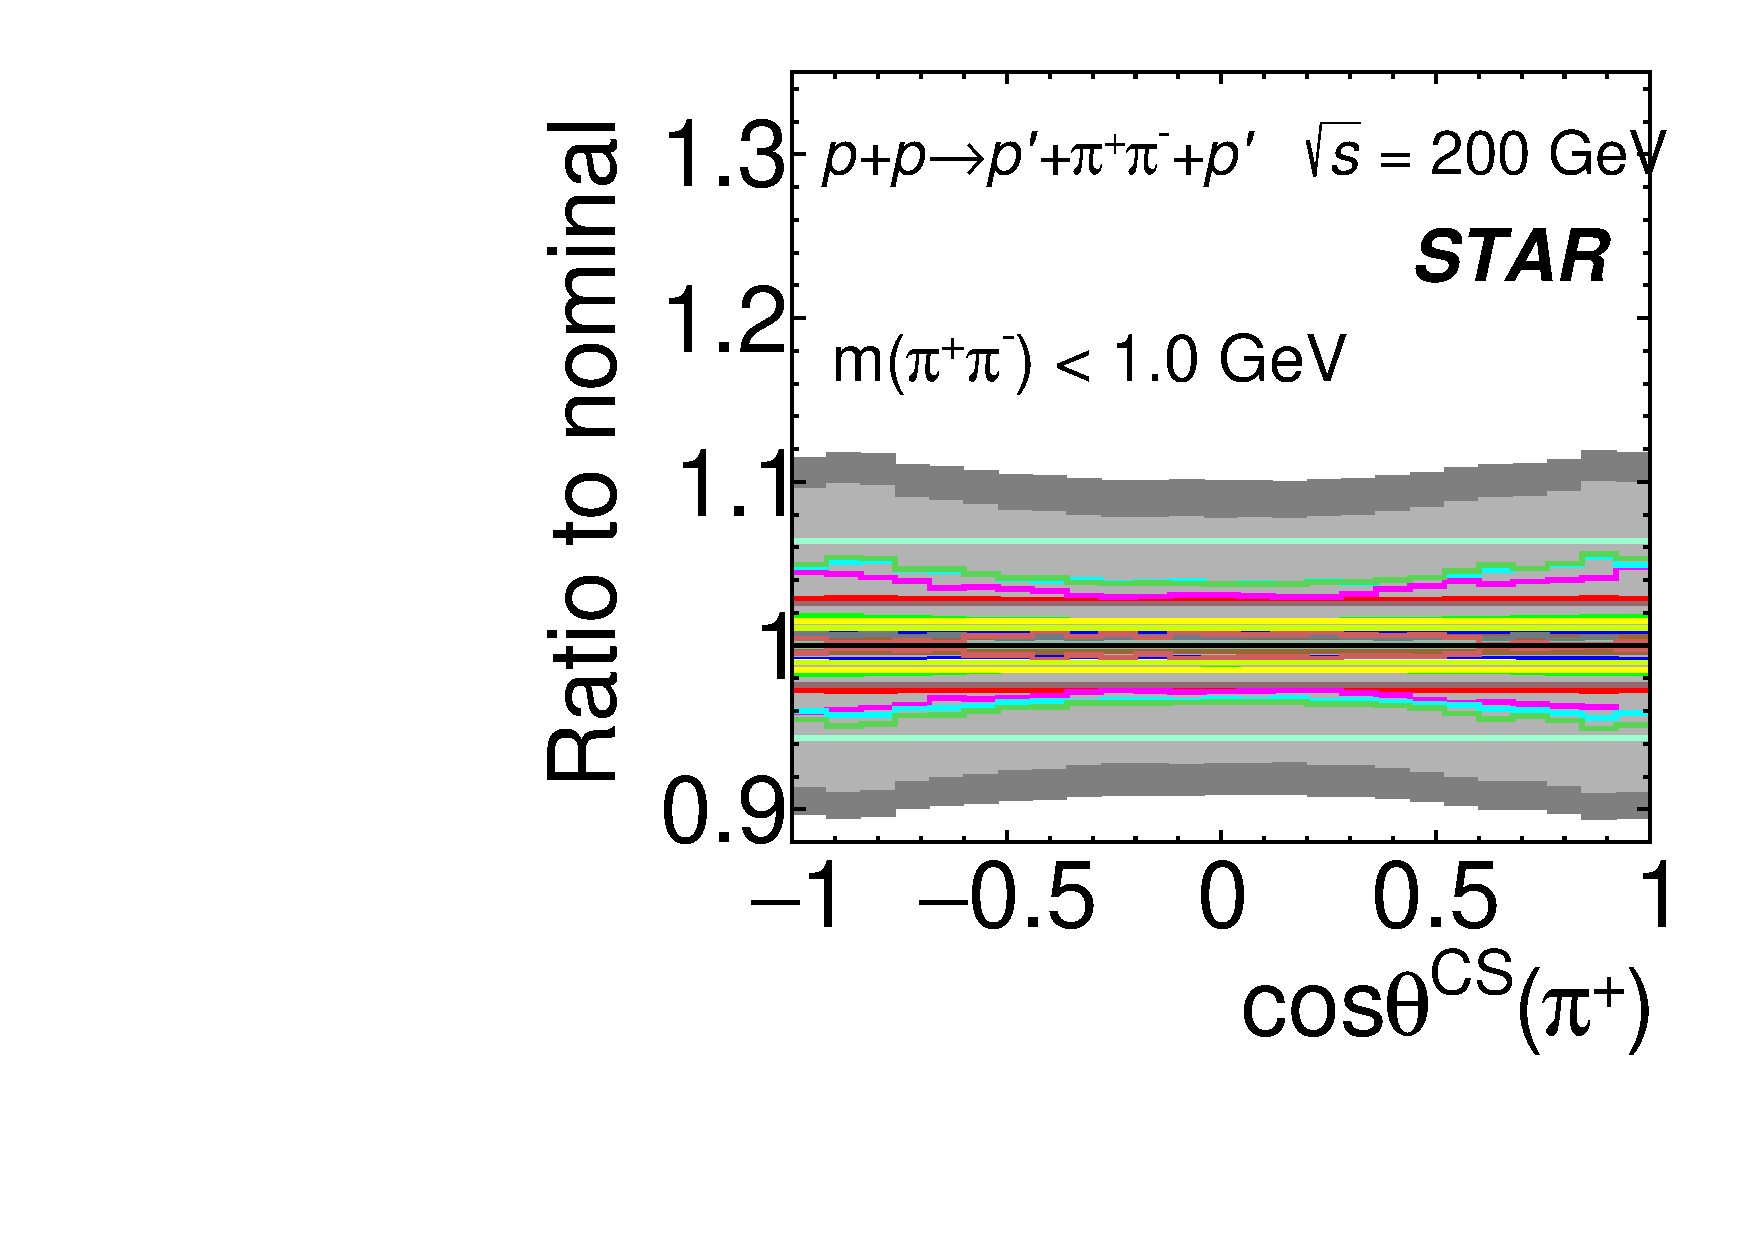
\includegraphics[width=.31\textwidth,page=1]{graphics/systematics/FinalResult_CosThetaCS_pion_MassBin_1_Systematics2.pdf}
\hfill
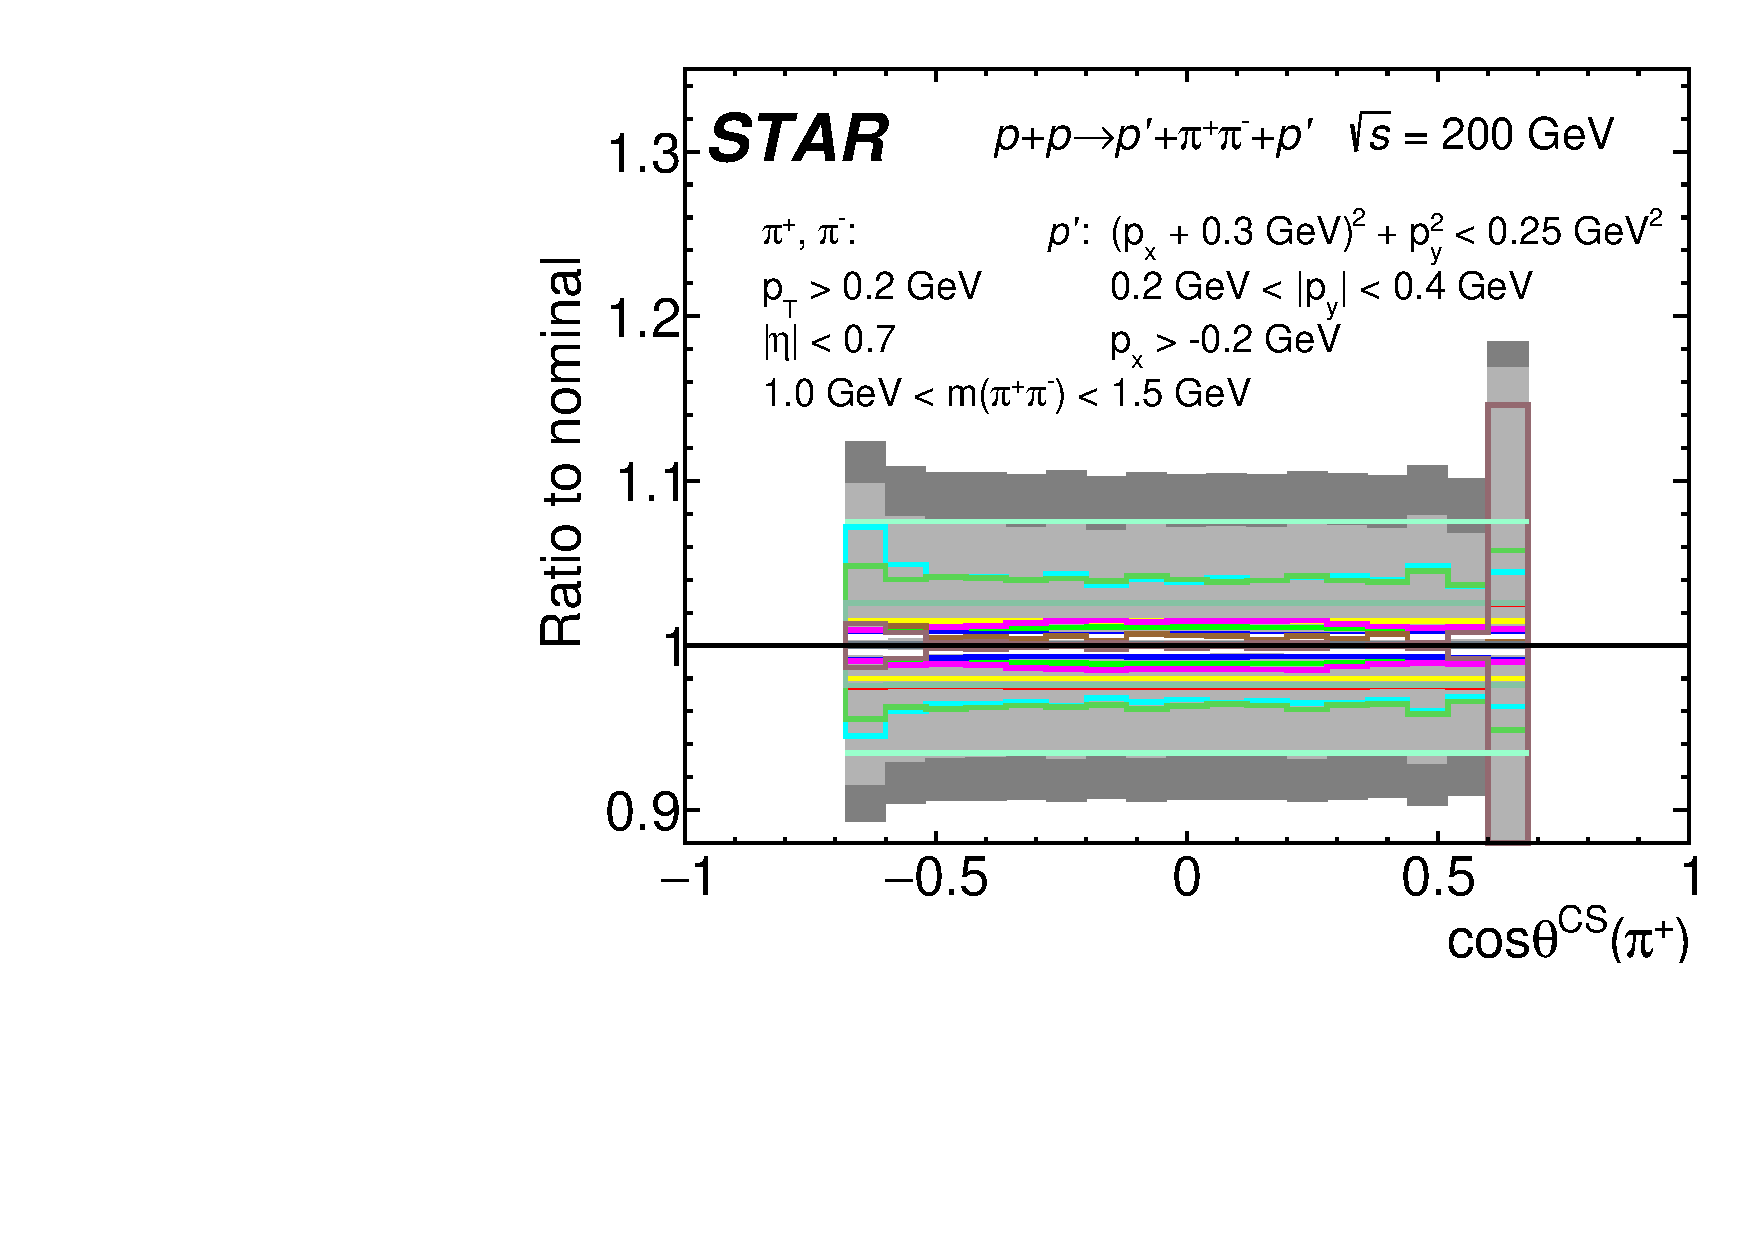
\includegraphics[width=.31\textwidth,page=1]{graphics/systematics/FinalResult_CosThetaCS_pion_MassBin_2_Systematics2.pdf}
\hfill
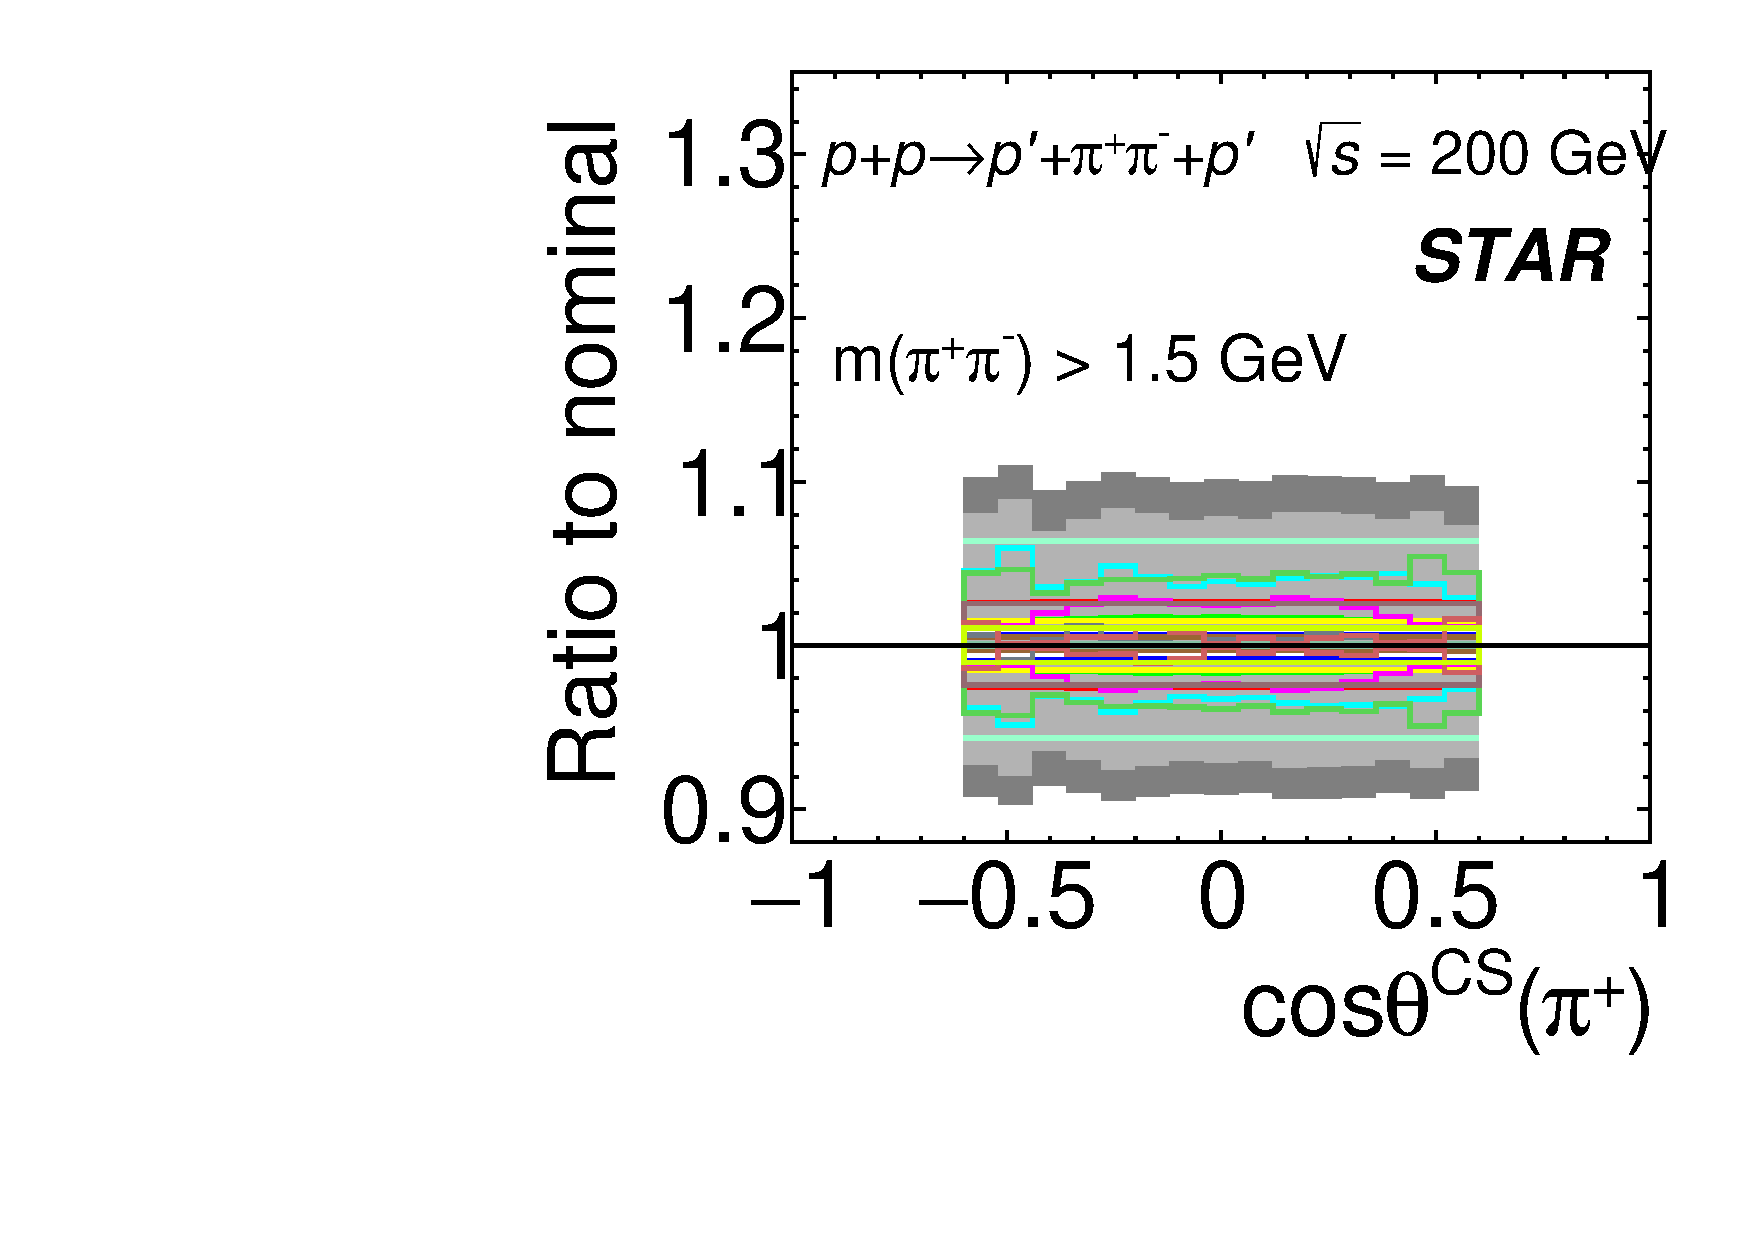
\includegraphics[width=.31\textwidth,page=1]{graphics/systematics/FinalResult_CosThetaCS_pion_MassBin_3_Systematics2.pdf}
\newline
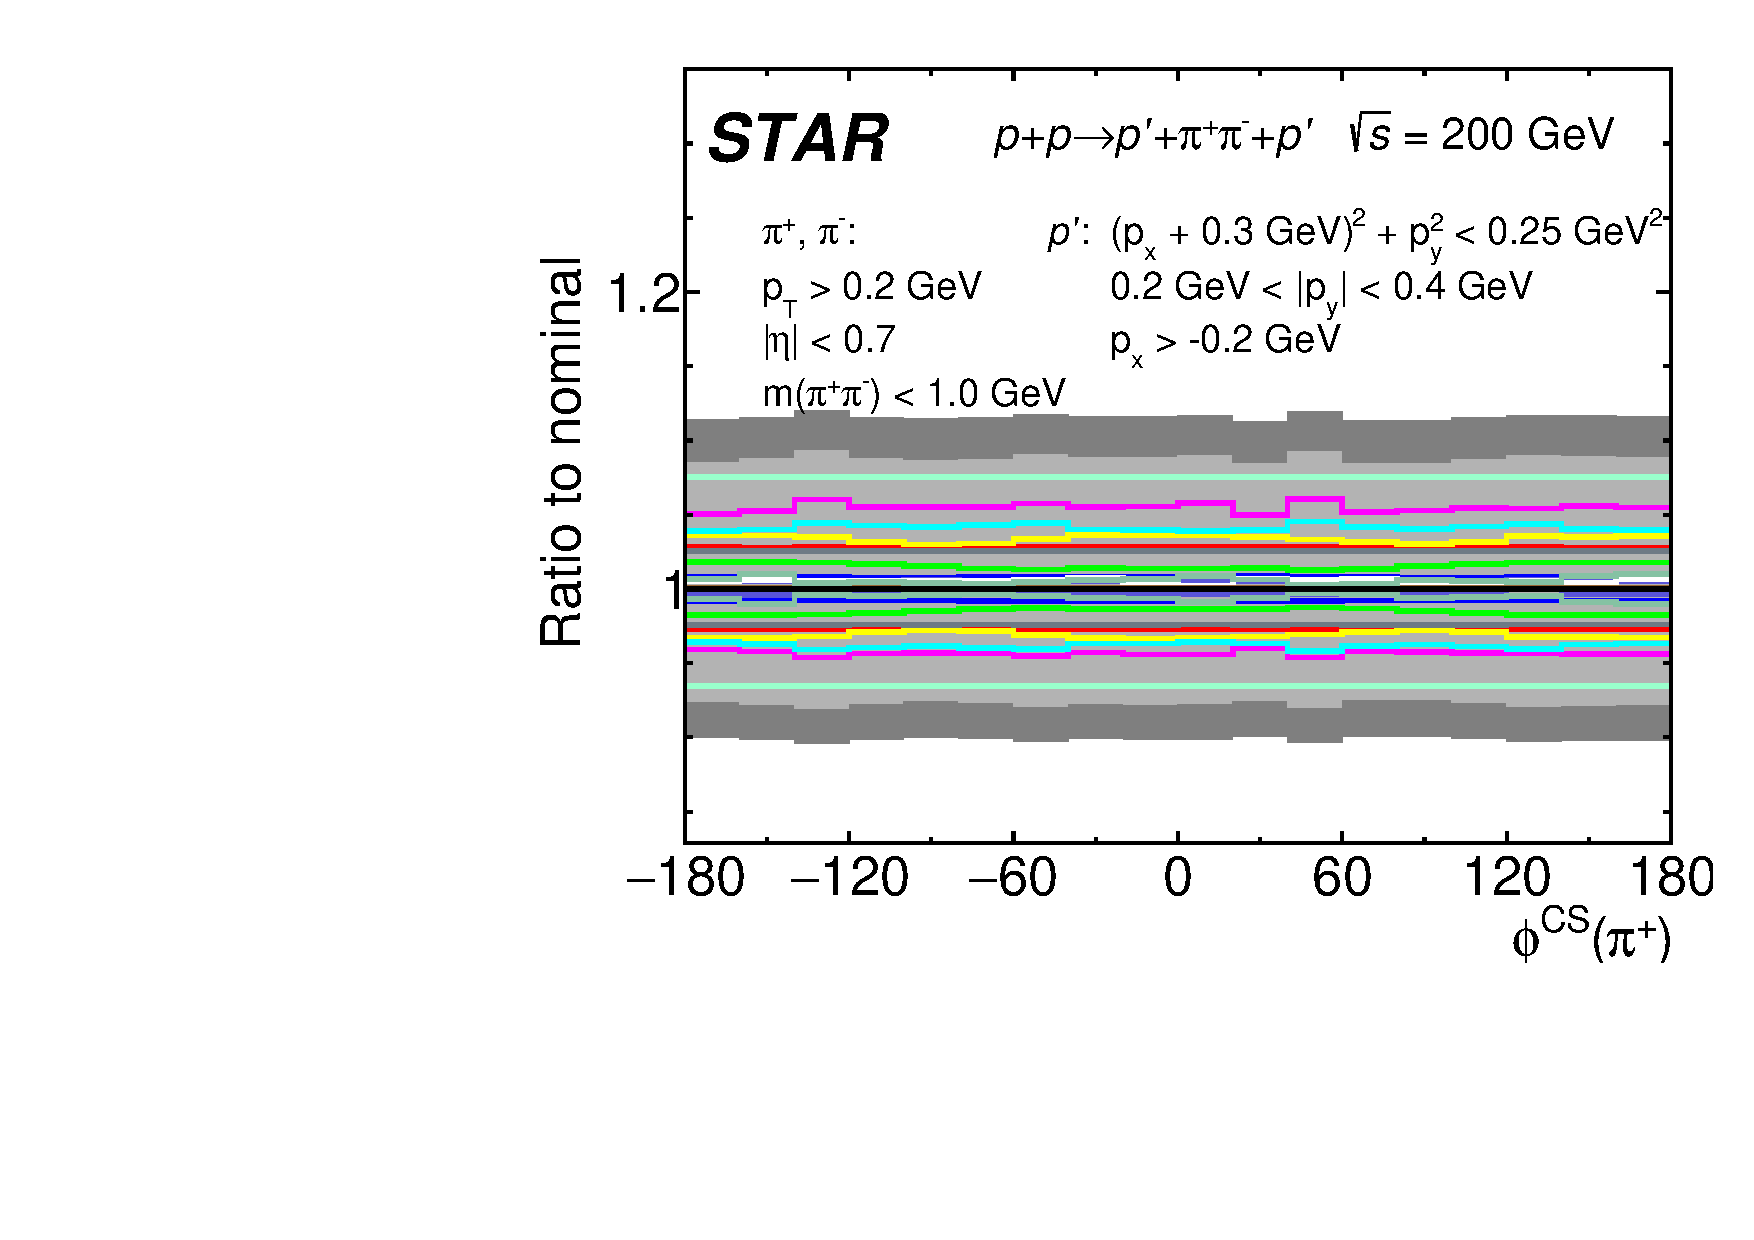
\includegraphics[width=.31\textwidth,page=1]{graphics/systematics/FinalResult_PhiCS_pion_MassBin_1_Systematics2.pdf}
\hfill
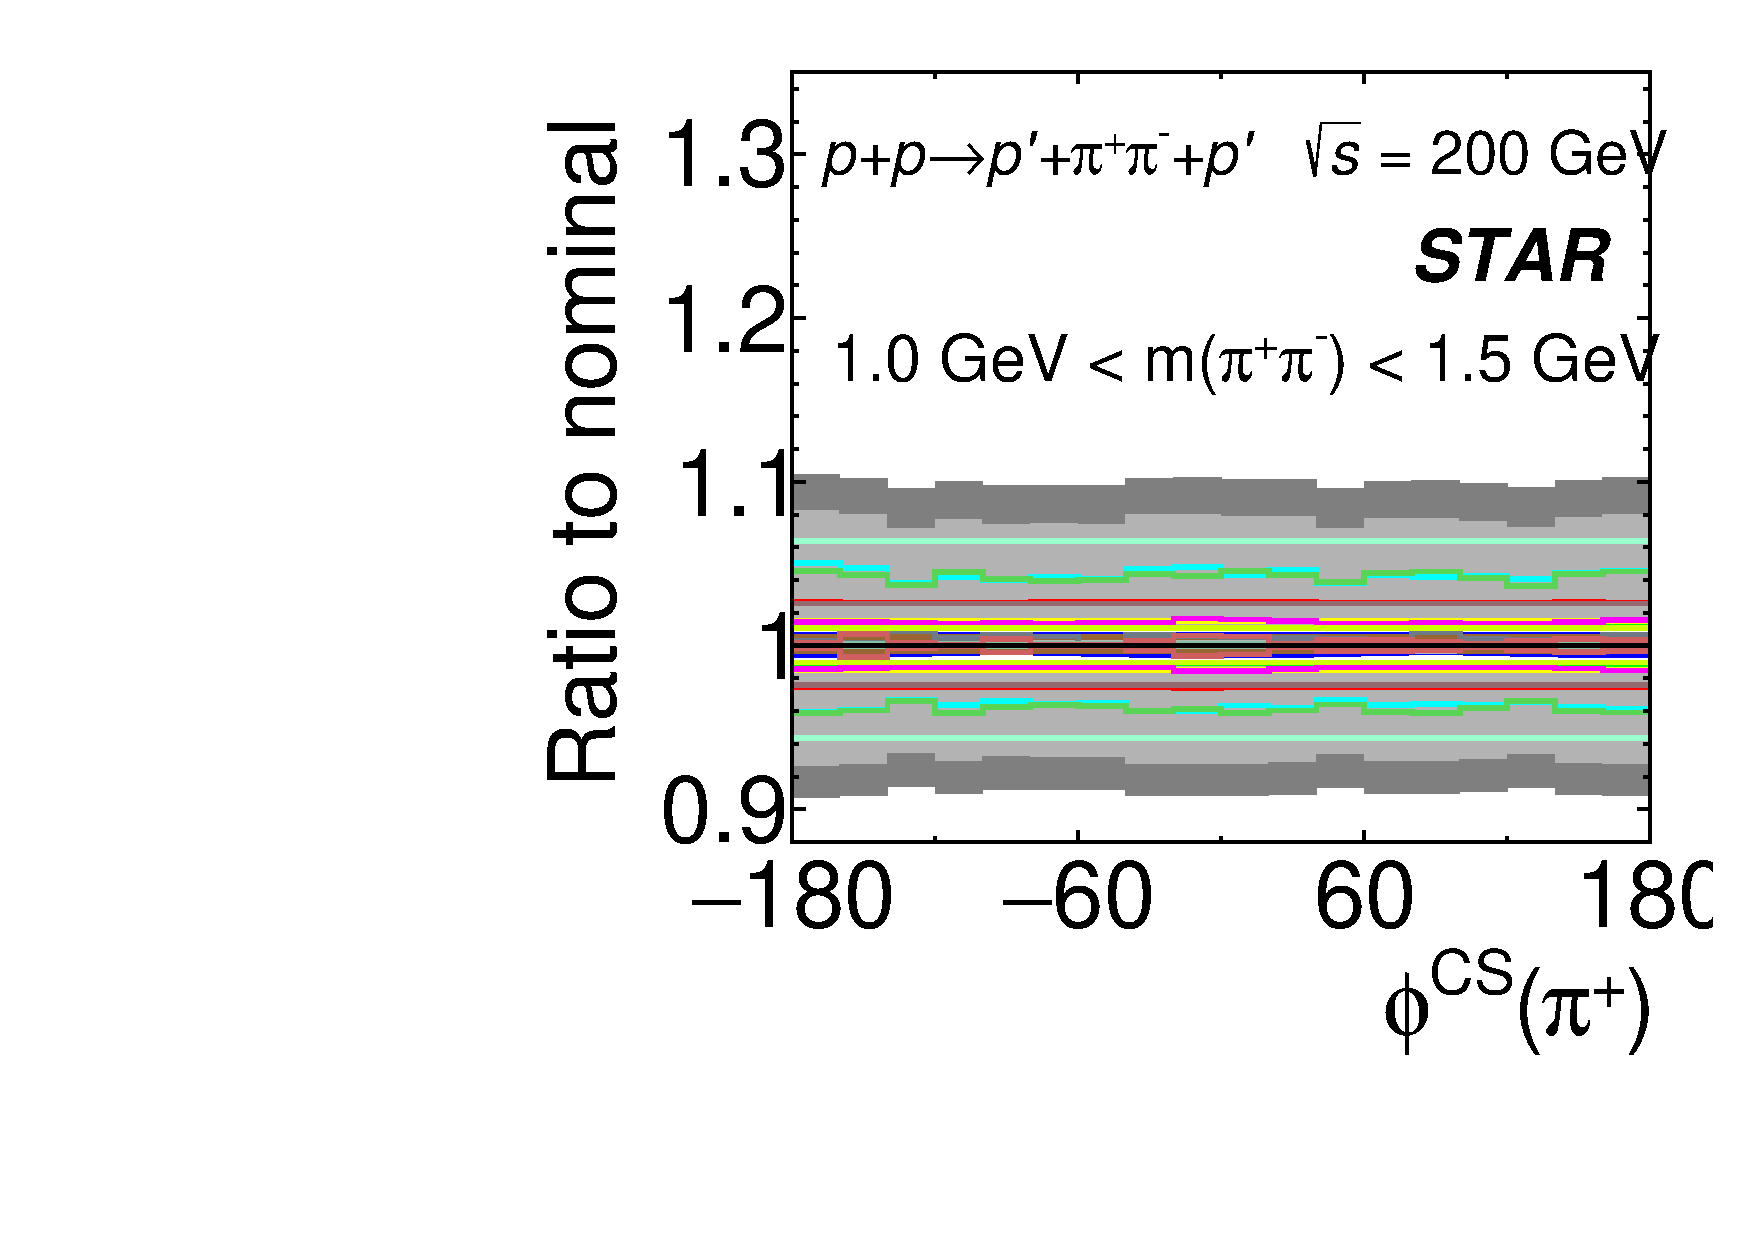
\includegraphics[width=.31\textwidth,page=1]{graphics/systematics/FinalResult_PhiCS_pion_MassBin_2_Systematics2.pdf}
\hfill
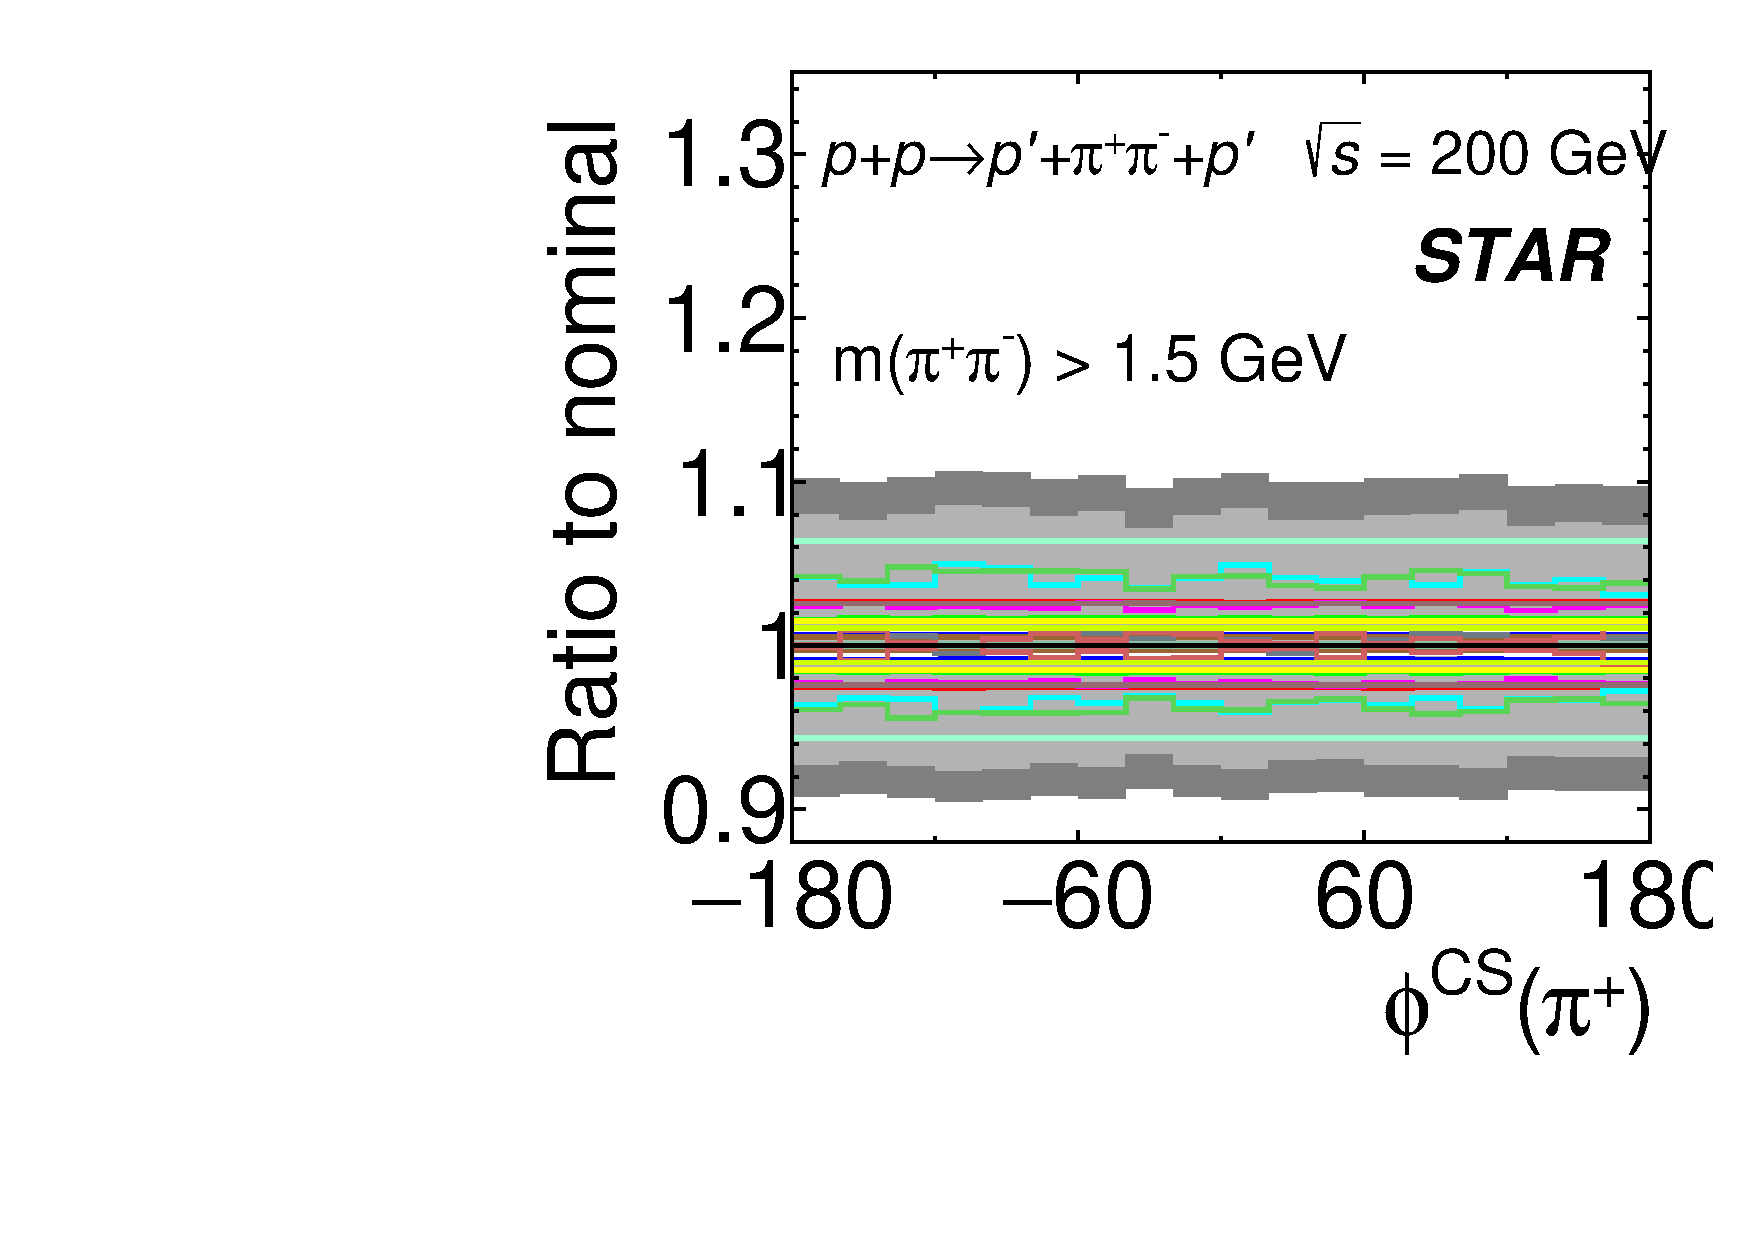
\includegraphics[width=.31\textwidth,page=1]{graphics/systematics/FinalResult_PhiCS_pion_MassBin_3_Systematics2.pdf}
%
\caption{Systematic uncertainties of the differential cross sections for CEP of $\pi^+\pi^-$ pairs as a function of $\cos{\theta^\mathrm{CS}}$ (top) and of $\phi^\mathrm{CS}$ (bottom)  measured in the fiducial region explained on the plots, separately for three ranges of the $\pi^+\pi^-$ pair invariant mass: $m<1$ GeV (left column), $1<m<1.5$ GeV (middle column) and $m>1.5$ GeV (right column).}
\label{systematics_7}
\end{figure}
